%&pdfLaTeX
% !TEX encoding = UTF-8 Unicode
\documentclass{article}
\usepackage{ifxetex}
\ifxetex
\usepackage{fontspec}
\setmainfont[Mapping=tex-text]{STIXGeneral}
\else
\usepackage[T1]{fontenc}
\usepackage[utf8]{inputenc}
\fi
\usepackage{textcomp}

\usepackage{graphicx}
\usepackage{array}
\usepackage{amssymb}
\usepackage{ulem}
\usepackage{fixltx2e}
\usepackage{amsmath}
\usepackage{amssymb}
\usepackage[T2A]{fontenc}
\usepackage[russian]{babel}
\usepackage{fancyhdr}
\renewcommand{\headrulewidth}{0pt}
\renewcommand{\footrulewidth}{0pt}

\pagestyle{fancy}
\rhead{}
\rfoot{}
\chead{}
\cfoot{}
\fancyfoot[LE]{\thepage{}}
\fancyfoot[LO]{\thepage{}}
\begin{document}

\begin{center}
Российская академия наук

Сибирское отделение

Институт динамики систем и теории управления
\end{center}

\begin{flushright}
На правах рукописи
\end{flushright}

\begin{center}
ПОПОВА Анастасия Константиновна\label{OLEHLINK10}\label{OLEHLINK11}

\textbf{ИНФОРМАЦИОННАЯ СИСТЕМА ДЛЯ ПОДДЕРЖКИ ПРИНЯТИЯ 
РЕШЕНИЙ ПО РАЦИОНАЛЬНОМУ ИСПОЛЬЗОВАНИЮ ЛЕСНЫХ 
РЕСУРСОВ }

Специальность 05.25.05 - Информационные системы 
и процессы, 

правовые аспекты информатики 

ДИССЕРТАЦИЯна соискание ученой степени 

кандидата технических наук
\end{center}

\begin{flushright}
Научный руководитель:

к.т.н. Черкашин Е.А.
\end{flushright}

\begin{center}
Иркутск - 2008
\end{center}

\emph{Введение \pageref{HToc199746714}}

\emph{Глава 1. Обзор подходов моделирования природных 
ресурсов и поддержки принятия решений \pageref{HToc199746715}}

\emph{1.1. Задача поддержки принятия решений и подходы 
к ее автоматизации \pageref{HToc199746716}}

\emph{1.2. Геоинформационные системы: обзор программных 
систем и приложений \pageref{HToc199746717}}

\emph{1.3. Программные комплексы для  моделирования 
лесных ресурсов: обзор \pageref{HToc199746718}}

\emph{Глава 2. Математическое обеспечение информационной 
системы \pageref{HToc199746719}}

\emph{2.1. Иерархическая система моделей лесных 
ресурсов \pageref{HToc199746720}}

\emph{2.1.1. Модель «Динамики управления древостоем» \pageref{HToc199746721}}

\emph{2.1.2. Модель «Лесные ресурсы» \pageref{HToc199746722}}

\emph{2.2. Технология создания  информационной 
системы \pageref{HToc199746723}}

\emph{Глава 3. Информационная система и ее инструментальные 
средства разработки специализированных приложений \pageref{HToc199746724}}

\emph{3.1. Назначение и область применения информационной 
системы \pageref{HToc199746725}}

\emph{3.2. Общая схема функционирования информационной 
системы \pageref{HToc199746726}}

\emph{3.3. Структура информационной системы \pageref{HToc199746727}}

\emph{3.3.1. Информационное обеспечение системы \pageref{HToc199746728}}

\emph{3.3.2. Представление моделей лесных ресурсов \pageref{HToc199746729}}

\emph{3.3.3. Реализация моделей лесных ресурсов \pageref{HToc199746730}}

\emph{3.3.4. Реализация численных расчетов \pageref{HToc199746731}}

\emph{3.3.5. База знаний \pageref{HToc199746732}}

\emph{3.3.6. Подсистема отображения результатов 
расчетов \pageref{HToc199746733}}

\emph{3.3.7. Формирование сценариев \pageref{HToc199746734}}

\emph{3.3.8. Сетевой доступ к информационной системе \pageref{HToc199746735}}

\emph{3.4. Инструментальные средства информационной 
системы \pageref{HToc199746736}}

\emph{3.4.1. Средства программирования пользовательских 
приложений \pageref{HToc199746737}}

\emph{3.4.2. Подсистема генерации карт и картографических 
анимаций \pageref{HToc199746738}}

\emph{3.4.3. Подсистема запросов к структуре моделей 
и расчетным данным \pageref{HToc199746739}}

\emph{Глава 4. Приложения информационной системы \pageref{HToc199746740}}

\emph{4.1. Моделирование динамики лесов Иркутской 
области по модели ДУД \pageref{HToc199746741}}

\emph{4.2. Моделирование динамики лесов Усть-Илимского 
района по модели «Лесные ресурсы» \pageref{HToc199746742}}

\emph{Заключение \pageref{HToc199746743}}

\emph{Список использованной литературы \pageref{HToc199746744}\label{HToc128995768}\label{HToc199746714}}

\section*{\textbf{Введение }}

Российская Федерация обладает большими запасами 
лесных ресурсов (ЛР), которые размещены неравномерно, 
местами истощены, а значительная часть территории 
страны относится к особо охраняемым территориям, 
где ведение хозяйственной деятельности ограничено. 
Значительная часть сибирских и дальневосточных 
регионов РФ  являются источником лесных ресурсов, 
которые составляют основную экспортную составляющую 
для этих регионов.

Проблема формирования политики использования 
ЛР является чрезвычайно важной задачей для 
лиц, принимающих решения (ЛПР) в управлении 
лесопромышленным регионом. ЛПР  в процессе 
принятия решения сталкивается с задачами, которые 
являются «антиинтуитивными». Под «антиинтуитивными» 
решениями понимаются решения, которые не являются 
«очевидно хорошими» на взгляд эксперта, т.е. 
решения, которые требуют специального исследования. 
Эффективность принимаемых ЛПР решений в первую 
очередь зависит от объема, вида и качества исходных 
данных о состоянии ЛР, а также прогнозов развития 
ЛР в зависимости от принимаемых ЛПР решений 
(политики заготовки ЛР). 

\textbf{Целью работы} является создание информационной 
системы (ИС) для ЛПР по рациональному использованию 
ЛР на основе компьютерного анализа и прогнозирования 
их состояния. Кроме того, целью работы являлась 
разработка инструментальных средств для создания 
специализированных приложений на основе компонент 
информационной системы.

\textbf{Основные задачи работы}.

1. Разработать методику конструирования информационной 
системы для ЛПР по рациональному использованию 
лесных ресурсов, основанную на комплексном 
подходе, включающем этапы идентификации математических 
моделей лесных ресурсов, расчета прогноза динамики, 
а также анализа критериев компьютерного моделирования.

2. Разработать подсистему идентификации моделей 
динамики и управления древостоем (ДУД) и «Лесные 
ресурсы».

3. Разработать инструментальные средства для 
конструирования интеллектных информационных 
систем для прогнозирования и анализа динамики 
ЛР на основе моделей.

4. Применить информационную систему для моделирования 
состояния лесных ресурсов Иркутской области.

\textbf{Структура работы.} Диссертация состоит 
из четырех глав, заключения и приложения. 

Во \textbf{введении} обосновывается актуальность 
темы диссертации, сформулированы основные 
положения и цель, а также задачи исследования. 
Обосновывается научная  новизна, практическая 
значимость, приводятся основные результаты 
работы.

В \textbf{первой главе} представлено описание существующих 
подходов к применению математического моделирования 
природных ресурсов в процессе поддержки принятия 
решений по рациональному ресурсопользованию.

Во \textbf{второй главе} приведено описание математического 
и программного обеспечения информационной 
системы по рациональному использованию лесных 
ресурсов, в том числе описание реализованных 
в системе математических моделей, технологии 
создания программного комплекса.

В \textbf{третьей главе} представлено описание 
программной реализации разработанной информационной 
системы и ее инструментальных средств разработки 
специализированных приложений. В п. 3.1 очерчивается 
область возможных применений информационной 
системы. П. 3.2 посвящен описанию схемы функционирования 
системы. Особенности реализации информационной 
системы описаны в п. 3.3. В п. 3.4. описана технология 
реализации инструментальных средств на основе 
информационной системы.

В \textbf{четвертой главе} описаны примеры использования 
информационной системы в области прогнозирования 
состояния лесных ресурсов Иркутской области.

В \textbf{заключении} приводится анализ полученных 
результатов, указываются направления дальнейшего 
развития информационной системы и разработанных 
инструментальных средств.

\textbf{Научная новизна }представленных в диссертации 
результатов состоит в следующем.

1. Разработана новая методика построения информационных 
систем для ЛПР, базирующаяся на прогнозировании 
состояния лесных ресурсов в зависимости от 
различных сценариев их использования. 

2. Создана оригинальная информационная система, 
использующая в качестве базовых математических 
моделей модели динамики управления древостоем 
(ДУД) и «Лесные ресурсы», впервые разработаны 
базы знаний для идентификации этих моделей 
по исходным данным распределения площадей 
лесов по породам и классам возраста. 

3. Разработаны оригинальные инструментальные 
средства для конструирования ИС для анализа 
состояния лесных ресурсов промышленного региона.

\textbf{Практическая значимость. }Созданная информационная 
система может использоваться при решении задач 
моделирования состояния лесных ресурсов различных 
регионов. В частности, она применялась для прогнозирования 
состояния лесных ресурсов Иркутской области 
и Усть-Илимского района, для которых были определены 
объемы рубок, позволяющие вести неистощительное 
использование ЛР.

Разработанные информационные системы апробированы 
на данных, предоставленных Институтом географии 
СО РАН.

Работа выполнена при поддержке РФФИ (гранты 
04-07-90227-в, 05-07-97201-р\_байкал\_в, 05-07-97204-р\_байкал\_в) 
и СО РАН (грант N 104).

\textbf{Основные защищаемые положения.} 

1. Разработана информационная система для исследования 
состояния лесных ресурсов промышленного региона 
ранга области, обеспечивающая анализ набора 
допустимых решений ЛПР. Указанный анализ осуществляется 
на основе результатов параметрической идентификации 
математических моделей ЛР, генерирования набора 
сценариев, расчета прогноза полученных сценариев, 
многокритериальной оптимизации набора сценариев 
и визуализации результатов в  ГИС.

2. Созданы базы знаний системы параметрической 
идентификации моделей ДУД и «Лесные ресурсы», 
позволяющие создавать представления идентифицированных 
моделей лесных ресурсов промышленного региона 
на основе имеющихся баз данных распределения 
площадей лесов по породам и классам возраста. 

3. Разработаны инструментальные средства, которые 
позволяют конструировать специализированные 
информационные системы, направленные на поддержку 
решений задач ЛПР, связанных с анализом состояния 
и перспектив использования ЛР промышленного 
региона.

4. Решены задачи прогнозирования ЛР Иркутской 
области с использованием  созданной информационной 
системы и инструментальных средств, определены 
максимальные объемы неистощительных рубок.

\textbf{Представление работы.} Основные положения 
и результаты докладывались на международных\label{OLEHLINK12}\label{OLEHLINK13}, 
всероссийских и региональных конференциях 
по математике и информатике:

1. Всероссийская конференция «Математические 
и информационные технологии в энергетике, экономике, 
экологии», г. Иркутск-Байкал, 12-19 июля 2003г. Е.А. 
Черкашин, А.К. Чудненко. «Создание интегрированных 
ГИС учета и прогнозирования динамики лесных 
ресурсов».

2. Всероссийская конференция «Инфокоммуникационные 
и вычислительные технологии и системы», г. Улан-Удэ-Байкал, 
5-9 августа 2003 г. И.В. Бычков, Е.А. Черкашин, А.К. 
Чудненко «Интегрированная ГИС учета и прогнозирования 
лесных ресурсов».

3. III школа-семинар молодых ученых, аспирантов 
и студентов г. Иркутска «Математическое моделирование 
и информационные технологии: управление, искусственный 
интеллект, прикладное программное обеспечение», 
Иркутск, оз. Байкал, 23-28 сентября 2003 г. Е.А. Черкашин, 
А.К. Чудненко. «Реализация интегрированных 
ГИС учета и прогнозирования динамики лесных 
ресурсов».

4. Научные чтения. 75-летие академика И.П. Дружинина, 
10 февраля 2004, ИСЭМ СО РАН, г. Иркутск. И.Н.\textsuperscript{ 
 }Владимиров, А.К. Чудненко. Прогнозирование 
пространственно-временной динамики лесных 
ресурсов Иркутской области с использованием 
ГИС-технологий. 

5. IV Байкальская школа-семинар молодых ученых 
«Математическое моделирование и информационные 
технологии: управление, искусственный интеллект, 
прикладное программное обеспечение, технологии 
программирования». Иркутск, оз. Байкал, 2004 г. 
А.К. Чудненко. Прогнозирование динамики лесных 
ресурсов Иркутской области с использованием 
ГИС-технологий. 

6. Байкальская Всероссийская конференция «Информационные 
и математические технологии», Иркутск, оз. Байкал, 
2004 г. Черкашин Е.А., Чудненко А.К. Программная 
система представления и обработки иерархических 
моделей лесных ресурсов. 

7. Международная конференция ИнтерКарто/ИнтерГИС 
10: устойчивое развитие территорий: геоинформационное 
обеспечение и практический опыт. Черкашин Е.А., 
Чудненко А.К., Владимиров И.Н. Интеллектная геоинформационная 
система динамики управления древостоем в контексте 
задачи разработки системы поддержки принятия 
решений по рациональному использованию лесных 
ресурсов. Владивосток (Россия), Чаньчунь (КНР), 
12-19 июня 2004 г.

8. Международная научная конференция ``Инфокоммуникационные 
и вычислительные технологии в науке, технике 
и образовании''. Чудненко А.К., Бычков И.В., Черкашин 
Е.А. Интеллектная геоинформационная система 
управления динамикой лесных ресурсов ИнГеС 
«Дилер», г. Ташкент, 28-30 сентября, 2004.

9. Научно-практическая конференция «Винеровские 
чтения». А.К. Чудненко Интеллектная геоинформационная 
система прогнозирования динамики лесных ресурсов. 
ИрГТУ, г. Иркутск, 21 октября 2004 г.

10. V школа-семинар молодых ученых «Математическое 
моделирование и информационные технологии: 
управление, искусственный интеллект, прикладное 
программное обеспечение, технологии программирования». 
 Иркутск, оз. Байкал, 2004 г. А.К. Чудненко «Создание 
интеллектной геоинформационной системы прогнозирования 
динамики лесных ресурсов».

11. VI школа-семинар молодых ученых «Математическое 
моделирование и информационные технологии: 
управление, искусственный интеллект, прикладное 
программное обеспечение, технологии программирования». 
Иркутск, оз. Байкал, 2005 г. Чудненко А.К. Инструментальные 
средства разработки программных систем анализа 
древостоев. 

12. VI Всероссийская конференция молодых ученых 
по математическому моделированию и информационным 
технологиям (с участием иностранных ученых), 
г. Кемерово, 29-31 октября 2005 г. Попова А.К. Разработка 
базы знаний для исследования развития лесных 
ресурсов.

13. VIII школа-семинар молодых ученых «Математическое 
моделирование и информационные технологии: 
управление, искусственный интеллект, прикладное 
программное обеспечение, технологии программирования». 
Улан-Удэ, оз. Байкал, 8-12 июля 2006 г. Попова А.К. 
Применение систем, основанных на формализованных 
знаниях, для исследования динамики лесных ресурсов.

14. Летний симпозиум «Научно-образовательный 
центр «Байкал» - стратегия развития» 3 - 7 июля 
2006  года, п. Большие Коты, Байкал, Россия. Попова 
А.К. Интеллектная ГИС прогнозирования динамики 
лесных ресурсов Иркутской области.

15. XII Байкальская Всероссийская конференция 
«Информационные и математические технологии 
в науке и управлении», г. Иркутск, 2007 г. Попова 
А.К. Инструментальное программное средство 
разработки СППР по рациональному использованию 
лесных ресурсов. 

16. IX школа-семинар молодых ученых ММИТ, г. Иркутск, 
2007 г. Попова А.К. База знаний СППР для прогнозирования 
состояния лесных ресурсов. 

17. Международная конференция геоинформатика: 
технологии, научные проекты, г. Иркутск, 2008 г. 
Попова А.К. Программная система прогнозирования 
динамики лесных ресурсов с использованием 
ГИС-технологий. 

\textbf{Публикации}. По теме диссертации опубликовано 
18 печатных работ [30-32, 35, 67-70, 92-96, 98-102] по списку 
литературы.

\textbf{Благодарности. }Автор благодарит к.т.н. 
Черкашина Е.А. за руководство диссертационной 
работой, а также д.г.н. Черкашина А.К., к.г.н. Владимирова 
И.Н. за консультации при реализации подсистемы 
математического моделирования ЛР. Особую признательность 
за помощь в работе, ценные замечания при выполнении 
работы и постоянную поддержку автор выражает 
чл.-к. РАН Бычкову И.В.\pagebreak{}\label{HToc199746715}

\section*{\textbf{Глава 1. Обзор подходов моделирования 
природных ресурсов и поддержки принятия решений}}

Информационная система предназначена для решения 
задач прогнозирования состояния лесных ресурсов 
на основе приложения системы математических 
моделей к конкретному природному объекту в 
условиях реализации некоторой потенциальной 
(гипотетической) политики использования лесных 
ресурсов, заданной набором параметров модели. 
В данном разделе рассматриваются основные 
существующие подходы к решению подобных задач.\label{HToc199746716}

\subsubsection*{\textbf{1.1. Задача поддержки принятия решений 
и подходы к ее автоматизации}}

При прогнозировании и планировании принимаются 
решения, связанные с выбором методов и средств, 
оценкой достоверности информации, выбором 
лучшего (с т.з. качественной оценки набора критериев) 
варианта прогноза и, как следствие, лучшего 
варианта плана решения поставленной управленческой 
задачи. Таким образом, задача принятия решений 
является с методологической и технологической 
точек зрения более общей, чем другие задачи 
управления. Для лица, принимающего решение 
(ЛПР), принятие решений является основной задачей, 
которую он обязан исполнять в процессе управления 
[41].  

Классификация задач принятия решений проводится 
по различным признакам. Наиболее существенными 
являются: степень определенности информации; 
использование эксперимента для получения информации; 
количество лиц, принимающих решения; содержание 
решений; направленность решений.

На процесс принятия решения часто воздействуют 
различные случайные параметры, усложняющие 
процедуру принятия решения. Недостаток информации 
об их распределении (сложность их измерения) 
приводит к необходимости принятия гипотез 
как об области  изменения данных параметров, 
так и о характере их распределения (о функции 
распределения вероятностей). Правильность 
используемых гипотез необходимо проверять 
с помощью методов оценки статистических гипотез. 
Проблемы принятия решений с недетерминированными 
параметрами называют проблемами принятия решений 
в условиях недостатка информации. Чем меньше 
информации об исследуемом объекте есть, тем 
больше может оказаться различие между ожидаемым 
и действительным результатами принимаемых 
решений в целом [41]. 

Современные системы поддержки принятия решения 
(СППР), возникшие как естественное развитие 
и продолжение управленческих информационных 
систем и систем управления базами данных, представляют 
собой системы, максимально приспособленные 
к решению задач повседневной управленческой 
деятельности, и являются инструментом, призванным 
оказать помощь ЛПР. С помощью СППР могут решаться 
неструктурированные и слабоструктурированные 
многокритериальные задачи.

СППР, как правило, являются результатом мультидисциплинарного 
исследования, включающего теории баз данных, 
искусственного интеллекта [53, 72], интерактивных 
компьютерных систем [73], методов имитационного 
моделирования [54, 76].

Ранние определения СППР (в начале 70-х годов 
ХХ века) отражали следующие три момента: 

1. возможность оперировать с неструктурированными 
или слабоструктурированными задачами, в отличие 
от задач, с которыми имеет дело исследование 
операций; 

2. интерактивные автоматизированные, т.е. реализованные 
на базе компьютера, системы; 

3. разделение данных и моделей. 

СППР являются человеко-машинными программными 
объектами, которые позволяют ЛПР использовать 
разнообразные методы (данные, знания, объективные 
и субъективные модели) для анализа и решения 
слабоструктурированных и неструктурированных 
задач. Идея СППР возникла как попытка автоматизации 
естественных человеческих действий по анализу 
имеющейся информации, планированию действий 
и т.п. с целью решения конкретной поставленной 
задачи.

В настоящее время нет общепринятого определения 
СППР, поскольку конструкция СППР существенно 
зависит от вида задач, для решения которых она 
разрабатывается, от доступных данных, информации 
и знаний, а также от пользователей системы. 

Будем понимать под СППР интерактивную автоматизированную 
систему, которая помогает ЛПР использовать 
имеющиеся данные и математические модели для 
идентификации и решения поставленных перед 
ним задач и принятия управленческих и других 
решений. 

Очень часто информационно-аналитические системы, 
создаваемые в расчете на непосредственное 
использование ЛПР оказываются чрезвычайно 
просты в применении, но жестко ограничены в 
объеме предоставляемых функций. Такие статические 
системы называются в литературе информационными 
системами руководителя (ИСР), или Executive Information 
Systems (EIS) [71, 106]. Они содержат в себе предопределенные 
множества запросов, и, будучи достаточными 
для повседневного обзора, ИСР, как правило, 
не способны ответить на вопросы, не предусмотренные 
исходной постановкой и набором функций. Т.е. 
каждый новый запрос, непредусмотренный при 
проектировании такой системы, должен быть сначала 
формально описан, изучен теоретически, разработан 
и закодирован программистом метод его решения, 
и только затем запрос может быть выполнен \label{OLEHLINK32}\label{OLEHLINK33}[74]. 
Время ожидания в таком случае может составлять 
часы и дни, что не всегда приемлемо для ЛПР. 

Динамические СППР, напротив, ориентированы 
на обработку нерегламентированных запросов 
аналитиков к данным. Работа аналитиков с этими 
системами заключается в интерактивной последовательности 
формирования запросов и изучения их результатов 
[48, 51].

В данной диссертационной работе программно 
реализуется следующая архитектура СППР [33] 
(рис. 1.1):

\begin{center}
\textbf{Машина}

\textbf{вывода}

\textbf{Подсистема искусственного интеллекта}

\textbf{Построение}

\textbf{математических}

\textbf{моделей}

\textbf{Многовариантное прогнозирование}

\textbf{Оценивание варианта решения}

\textbf{Генератор}

\textbf{решений}

\textbf{Лицо,}

\textbf{принимающее }

\textbf{решение}

\textbf{Система}

\textbf{поддержки}

\textbf{принятия }

\textbf{решения}

\textbf{Описание постановки задачи}

\textbf{Данные}

\textbf{База}

\textbf{знаний}\fancyfoot[LE]{\thepage{}}
\fancyfoot[LO]{\thepage{}}

Рис. 1.1. Архитектура СППР
\end{center}

Основной частью СППР является генератор решений 
(рис. 1.1), который действует на основании исходных 
данных (блок «Данные») об объекте исследования 
и описания постановки задачи. В процессе принятия 
решения генератор решений взаимодействует 
с подсистемой искусственного интеллекта, которая, 
в свою очередь, использует базу знаний для построения 
базовой структуры модели объекта исследования 
по известным исходным данным [18]. Также в базу 
знаний включаются разделы, формализующие некоторые 
способы изменения состояния объекта, и эвристики, 
используемые математиком-исследователем в 
процессе построения модели, что обеспечивает 
подстройку модели к специфическим свойствам 
объекта. Таким образом, подсистема искусственного 
интеллекта используется для идентификации 
математической модели объекта и оценивания 
вариантов решения [33, 81].

На этапе идентификации модели используются 
данные об исследуемом объекте, которые хранятся 
в базе данных (БД). В базе знаний хранятся знания 
эксперта об особенностях объекта исследования 
[3, 10, 28]. Далее  производится идентификация параметров 
модели объекта исследования, вычисление начальных 
условий, по выбранной модели рассчитываются 
прогнозы состояния объекта [7]. При этом могут 
просчитываться различные сценарии динамики 
объекта, в зависимости от комбинации начальных 
параметров. 

\begin{center}
\textbf{Исследуемый}

\textbf{объект}

\textbf{Модель}

\textbf{исследуемого}

\textbf{объекта}

\textbf{Модуль}

\textbf{идентификации}

\textbf{модели}

\textbf{База}

\textbf{знаний}
\end{center}

%%\begin{figure}[htbp]
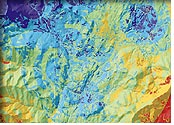
\includegraphics[width=94pt, height=68pt, keepaspectratio=true]{asyaDisser9_3-fig001.jpg}
%%\caption{This should be the caption for \texttt{asyaDisser9\_3-fig001.jpg}.}
%%\end{figure}

\fancyfoot[LE]{\thepage{}}
\fancyfoot[LO]{\thepage{}}

\begin{center}
Рис. 1.2. Прогнозирование динамики пространственно-распределенного 
объекта в СППР\label{OLEHLINK6}\label{OLEHLINK7}
\end{center}

Рассчитываются критерии анализа сценариев, 
над которыми далее проводится многокритериальная 
оптимизация (МКО) [27]. МКО требуется для сужения 
исходного набора сценариев по заданному набору 
критериев [40, 97]. Если результаты расчетов имеют 
пространственную привязку, то они отображаются 
по запросу пользователя в виде картографического 
произведения [43, 65] (рис. 1.2).

Отображение данных на карте производится при 
помощи модуля ГИС. Он позволяет посмотреть 
проекцию состояния объекта исследования в 
любой момент времени из интервала прогнозирования. 
Наличие модуля ГИС является особенностью разработанной 
в диссертации СППР и инструментальных средств 
создания СППР.

В соответствие с принятой нами архитектурой 
СППР (рис. 1.1) основную часть в реализации систем 
поддержки принятия решений составляет программное 
обеспечение расчета прогноза на основе математических 
моделей. \label{HToc199746717}

\subsubsection*{\textbf{1.2. Геоинформационные системы: 
обзор программных систем и приложений}}

Географическая информационная система, ГИС 
- информационная система, обеспечивающая сбор, 
хранение, обработку, доступ, отображение и распространение 
пространственно-распределенных данных. Она 
содержит данные о пространственных объектах 
в форме их цифровых представлений (векторных, 
растровых, квадротомических и иных), включает 
соответствующий задачам набор функциональных 
возможностей, в которых реализуются операции 
геоинформационных технологий, поддерживается 
программным, аппаратным, информационным, нормативно-правовым, 
кадровым и организационным обеспечением [47]. 

Геоинформационное обеспечение является главной 
составляющей ГИС - комбинации интерактивной 
графической системы с банком данных, в котором 
хранятся как геометрические (в виде цифровых 
топографических или специальных планов), так 
и предметные данные геометрических объектов 
(в виде текстовой  информации), являющиеся моделью 
реальной городской среды. Источниками информации 
служат топографические карты, результаты измерений 
и различного рода алфавитно-цифровые документы.

Современные ГИС в их классическом [38, 44-47, 85] 
понимании ориентированы на хранение и отображение 
пространственно-распределенной информации 
и широко используются для оценки ресурсно-экологического 
потенциала лесов.

Функциональное расширение процедурных возможностей 
ГИС превращает их в интегрированные информационные 
системы. В узком смысле интегрированные ГИС 
(ИГИС) совмещают собственно ГИС и системы цифровой 
обработки изображений (например, данные дистанционного 
 зондирования) [44]. Разновидность интегрированных 
информационных систем - интегрированные экспертные 
системы [64, 66, 78] - включают помимо базы знаний 
[36-37, 39, 62] и средств оперирования с ними базы 
данных и базы моделей. Поэтому в обобщенном 
смысле интегрированная ГИС должна представлять 
собой целостную систему разнообразных информационных 
баз и средств анализа информации, которая в 
широком смысле не зависит от ее содержания 
[71, 74, 88].

В настоящее время существует и используется 
в работе множество разнообразных ГИС-пакетов. 
Хорошо себя зарекомендовали в обработке мелкомасштабных 
карт (геология, сельское хозяйство, навигация, 
экология и т.п.) такие ГИС, как \textit{ArcInfo} и \textit{ArcView 
GIS}. Обе системы разработаны компанией ESRI и широко 
распространены в мире. 

Самый популярный и распространенный программный 
продукт ESRI  \textit{ArcView GIS} выполнен в виде стандартного 
приложения WINDOWS, он работает также на платформах 
UNIX и в ряде версий Macintosh. Он легок в освоении 
и может использоваться в различных сферах деятельности 
для визуализации, запроса и анализа любой пространственной 
информации. \textit{ArcView GIS} итегрирует векторные, 
растровые, табличные данные в единую аналитическую 
систему.

ГИС \textit{ArcView }позволяет:

\ensuremath{-} создать и поддерживать географическую 
базу данных;

\ensuremath{-} использовать данные из других ГИС, 
в том числе обращаться к серверным базам данных 
посредством SQL-запросов;

\ensuremath{-} использовать растровые данные в процессе 
картографического анализа и отображения;

\ensuremath{-} управлять картографическими проекциями, 
масштабом и единицами измерений;

\ensuremath{-} создавать картографические произведения 
из готовых данных;

\ensuremath{-} реализовывать на основе встроенного 
набора функций новые программные пакеты, ориентированные 
на решение специальных задач; данные пакеты 
реализуются с помощью встроенного языка программирования 
\textit{Avenue}.

Средствами разработки \textit{ArcView} пользователь 
может, кроме прочего, программировать алгоритмы 
расчета математических моделей  исследуемых 
процессов, алгоритмически рассчитывать необходимые 
коэффициенты на основе имеющихся баз данных. 

Для \textit{ArcView} реализован модуль \textit{Spatial Analyst}, 
имеющий широкий набор средств обработки пространственных 
данных, проведения их совместного растрово-векторного 
анализа. С его помощью можно построить модель 
местности, построить изолинии, определить уклоны 
и экспозиции, создать буферные зоны по заданным 
параметрам вокруг одного или группы объектов, 
провести анализ близости и зонирование.

Другая ГИС ESRI \textit{ARC/INFO} предоставляет полный 
набор средств и функций для управления, анализа, 
отображения и картирования географической 
информации. Типичными сферами применения \textit{ARC/INFO} 
являются:

\ensuremath{-} создание баз данных, анализ деятельности, 
управление генеральными планами развития небольших 
городов; 

\ensuremath{-} создание картографической продукции 
для разнообразных нужд; 

\ensuremath{-} картирование и анализ пространственно 
распределенной информации. 

В состав ГИС \textit{ARC/INFO} входит шесть интегрированных 
модулей:

\ensuremath{-} PC~STARTER~KIT~- базовые средства создания 
ГИС, включающие системы оцифрования, топологической 
поддержки данных, поддержки картографических 
проекций, а также системы работы с базами данных 
и визуализации для вывода твердых копий. 

\ensuremath{-} PC~ARCPLOT~-~~средства графического отображения 
информационных запросов и вывода картографической 
информации - от простых экранных изображений 
до высококачественных географических карт 
для докладов и презентаций. 

\ensuremath{-} PC~ARCEDIT~- ввод и редактирование графических 
и атрибутивных данных, включающее средства 
проверки и корректировки ошибок. 

\ensuremath{-} PC~DATA~CONVERSION~- импорт/экспорт векторных 
данных. 

\ensuremath{-} PC~OVERLAY~- средства объединения и анализа 
географической информации на основе пространственной 
и топологической взаимосвязи объектов. 

\ensuremath{-} PC~NETWORK~- анализ и моделирование пространственных 
сетей: дорожных, речных, газовых, электрических 
и т.п.

ГИС \textit{MapInfo }спроектирован для обработки и 
анализа информации, имеющей адресную или пространственную 
привязку. Операции, поддерживающие взаимодействие 
с базой данных, достаточно просты, что  требует 
от пользователя только базовых знаний для обеспечения 
доступа к внешним БД; в то время как пользователь, 
в конечном счете, получает мощные возможности 
компьютерной картографии для решения своих 
задач. В дополнение к традиционным для СУБД 
функциям, \textit{MapInfo} позволяет собирать, хранить, 
отображать, редактировать и обрабатывать картографические 
данные, хранящиеся в базе данных, с учетом пространственных 
отношений объектов.

Встроенный язык запросов SQL, благодаря географическому 
расширению, позволяет организовывать выборки 
с учетом пространственных отношений объектов, 
таких как удаленность, вложенность, перекрытия, 
пересечения, площади объектов и т.п. Сочетание 
тематических слоев и методов буферизации, районирования, 
слияния и разбиения объектов, пространственной 
и атрибутивной классификации позволяет создавать 
синтетические многокомпонентные карты с иерархической 
структурой легенды. Система снабжена средством 
программирования \textit{MapBasic}.

В последнее время активно развивается направление 
интеллектуализации ГИС. Среди известных зарубежных 
и отечественных разработок обработки пространственно-распределенных 
данных, использующих средства и методы искусственного 
интеллекта,  можно выделить системы MEXES и ЭПСЛА.

ГИС \textit{MEXES (К. Fedra)}[8] можно отнести к интеллектным 
ГИС. Данные в системе представляются с помощью 
специальных дескрипторов, содержащих качественную 
и количественную информацию о некотором параметре 
объекта исследования. Также дескрипторы включают 
информацию о возможных источниках получения 
данных, это может быть либо запрос к базе данных, 
либо результат выполнения таблицы принятия 
решения, либо результат выполнения правила, 
либо вопрос к пользователю. Название параметра, 
синонимы, тип параметра, единицы измерения, 
список, к которому принадлежит параметр, названия 
диапазонов значений составляют совокупность 
качественной информации о параметре. В качестве 
диапазонов значений дискретных интервальных 
шкал используются качественных характеристик, 
таких как \texttt{"}незначащий\texttt{"}, \texttt{"}малый\texttt{"}, 
\texttt{"}средний\texttt{"}, \texttt{"}большой\texttt{"}, \texttt{"}значительный\texttt{"}, 
что демонстрирует похожесть данного подхода 
с нечеткой логикой. К количественной информации 
относятся конкретные значения качественных 
диапазонов.

ГИС MEXES предназначена для оценки влияния антропогенных 
факторов на природные ресурсы, в частности 
на водные ресурсы. Примером решаемой задачи 
является рассмотренная в [8] \texttt{"}Задача размещения 
индустриального объекта\texttt{"}.  

Знания представляются в системе в виде продукций 
вида \texttt{"}Если \texttt{<}Условие\texttt{>} То \texttt{<}Действие\texttt{>}\texttt{"}, 
где условие содержит пропозициональное логическое 
выражение, а действие - последовательность 
операторов присваивания значений новым переменным 
и операторов модификации дескрипторов.

К достоинствам системы можно отнести простоту 
представления знаний и данных, обеспечиваемую 
продукционным формализмом представления знаний 
и способом представления данных об объекте 
в виде дескрипторов, а также разрешимый пропозициональный 
логический вывод, гарантирующий ответ системы. 
Во многих задачах такой подход достаточно эффективен, 
однако для решения более сложных  задач, например, 
задач анализа состояния объекта во времени, 
выразительности пропозиционального языка 
недостаточно. 

Дальнейшее развитие системы осуществляется 
в направлении использования языка Пролог, в 
том числе для пространственного анализа местности 
на \texttt{"}приспособленность\texttt{"} к размещению 
того или иного объекта, а также языка ЛИСП и 
классического фреймового представления знаний 
о системе

В ГИС \label{HToc28945737}\textit{ЭСПЛА (ИВМ СО РАН) } применяется 
подобный механизм как и в предыдущей гибридной 
ГИС, но с некоторыми отличиями. ГИС ЭСПЛА предназначена 
для построения сценария действий по ликвидации 
существующей или гипотетической чрезвычайной 
ситуации (ЧС). Сценарием развития ЧС называется 
процесс изменения некоторой исходной ситуации 
в дискретном времени и пространстве под воздействием 
событий ЧС. Каждый сценарий характеризуется 
набором параметров, например, временем развития 
ЧС, которое необходимо свести к минимуму. Каждый 
новый шаг сценария строиться на основе предыдущего 
шага применением к нему программной процедуры, 
базирующейся на продукционно-фреймовой объектно-ориентированной 
модели представления данных и знаний.

Представление данных в системе опирается на 
классическое фреймовое представление с использованием 
слотов-демонов как источников получения значений 
соответствующих слотов фрейма. Основным достоинством 
в рассматриваемой системе является существенное 
расширение языка - применение нечетких механизмов 
в представлении продукций, однако данных подход 
имеет те же недостатки как и у системы MEXES. Система 
ЭСПЛА и ее механизмы в значительной мере ориентированы 
на свою предметную область, хотя при ликвидации 
некоторых специфических свойств (ориентированность 
на сценарный подход, необходимость сообщения 
оценки шага сценария, и т.п.) возможно использование 
и для более широкого класса задач. 

Этот обзор показывает, что современные ГИС 
обладают как библиотеками средств моделирования 
пространственных данных, ориентированными 
на определенные задачи, так и необходимым инструментарием 
реализации модулей для решения других задач. 
 Также некоторые ГИС содержат базы знаний о 
предметной области, позволяющие проводить 
достаточно эффективный поиск решения для ЛПР.\label{HToc199746718}

\subsubsection*{\textbf{1.3. Программные комплексы для  
моделирования лесных ресурсов: обзор}}

В моделировании динамики леса имеется ряд особенностей, 
связанных со спецификой его развития - длительностью 
протекания процессов в древостоях, измеряемой 
несколькими десятками и сотнями лет, а также 
большим разнообразием видовой и возрастной 
структуры лесонасаждений, разными масштабами 
информационного обобщения и принятия решений. 

Математическое моделирование динамики лесов 
имеет длительную историю [91]. Первыми моделями 
по праву считаются таблицы хода роста лесонасаждений, 
которые и в настоящее время широко используются 
в лесоводственной практике. При построении\textsuperscript{ 
}этих таблиц применяются математико-статистические 
методы обработки данных. Материалы таблиц легли 
в основу многих математических моделей, среди 
которых наиболее известны модели Г. Ф. Хильми 
[82-83].

Лесная растительность описывается математическим 
языком на различных уровнях ее организации 
с разной степенью детальности: строятся модели 
фотосинтеза древесных пород [5, 24], лес включается 
как компонент в модели биосферы [57-59]. Разнообразен 
также математический аппарат моделирования. 
Помимо математико-статистических методов анализа 
изменения структуры лесонасаждений большое 
распространение при моделировании леса получили 
элементы теории случайных марковских процессов 
[17, 19], используются системы простых дифференциальных 
уравнений и дифференциальных уравнений в частных 
производных [1-2].

В лесной науке разработаны достаточно развитые 
системы математического моделирования динамики 
лесов на различных уровнях их организации: 
локальном - модели отдельного дерева и древостоев 
[4-5, 9, 12-13, 23, 26, 49, 60]; субрегиональном - описание 
изменения распределения лесных площадей по 
породам и классам возраста, стадиям восстановительной 
динамики [20-21, 25, 63, 77, 89, 91]; региональном - уравнения 
перераспределение запасов биомассы по породам 
[15-16, 90] и глобальном - отражение роли и места 
лесных экосистем в кругообороте вещества и 
энергии [58].

В отличие от моделей других авторов (Г.П.Карев, 
М.Д. Корзухин, Ф.Н. Семеневский, В.Л. Недорезов, 
Г.Ф. Хильми, D.B. Botkin, L.M. Peden, J.S. Williams, W.E. Frayer, H.H. 
Shugart), имитирующих либо качественные особенности 
поведения природных систем, либо количественную 
динамику отдельных объектов, используемые 
в реализованной информационной системе модели 
позволяют достаточно точно давать прогнозы 
качественных и количественных характеристик 
лесных экосистем независимо от их местоположения. 
Это достигается за счет того, что в моделях 
используются фундаментальные закономерности 
динамики лесных экосистем, неизвестные раннее, 
и оригинальный ландшафтно-типологический подход, 
позволяющий связать структурные изменения 
в лесах с конкретным местоположением.

В настоящее время подавляющее большинство 
лесоустроительных предприятий для создания 
лесных карт используют ГИС и их технологии. 
ГИС \texttt{"}\textit{TopoL-L}\texttt{"} - программный комплекс, 
позволяющий выполнять весь комплекс работ 
по созданию, редактированию, анализу и использованию 
лесных цифровых карт [52]. В состав  комплекса 
 \texttt{"}TopoL-L\texttt{"}  входит  собственно ГИС \texttt{"}\textit{TopoL}\texttt{"} 
(TopoL Software, s.r.o., Чехия), являющейся универсальной 
геоинформационной системой и программа \texttt{"}\textit{ЛесИС}\texttt{"} 
(Лесная информационная система), которая обеспечивает 
весь комплекс работ с атрибутивными данными 
(таксационные описания, учет лесного фонда 
и т.п.). ЛесИС разрабатывается ООО \texttt{"}ЛЕСИС\texttt{"}, 
которое учреждено группой разработчиков ГИС 
Центрлеспроекта.

Программный комплекс ЛесИС позволяет:

\ensuremath{-} создавать лесные карты разного масштаба;

\ensuremath{-} привязывать к ним семантическую информацию;

\ensuremath{-} осуществлять быстрый поиск информации 
в пределах лесхоза или региона по запросам 
любой сложности или вложенности, по любым показателям:

\ensuremath{-} просматривать карты и связанную с ними 
таксационную или учетную информацию в любых 
режимах и последовательности:

\ensuremath{-} вносить по результатам хоздеятельности 
текущие изменения как в пространственную, так 
и в таксационную информацию;

\ensuremath{-} получать на основе таксационных описаний 
итоги по кварталам, лесничествам, лесхозам 
или по произвольно отобранным объектам, в т.ч. 
учет лесного фонда;

\ensuremath{-} получать любые тематические карты.

Интерфейс программы ориентирован на отраслевые 
задачи. Меню содержат только те пункты, которые 
необходимы пользователю - сотруднику лесной 
отрасли. 

Интерфейс спроектирован в одном стиле для рабочих 
мест любого уровня управления. Лесничий и сотрудник 
регионального управления видят на экране одни 
и те же инструменты, окна, пользуются стандартными 
приемами работы, хотя характер информации у 
каждого из них может сильно отличаться. 

Информация разной степени обобщения (повыдельная 
или в целом по лесхозу) доступна на любых рабочих 
местах. Для этого достаточно просто иметь ее 
на компьютере конкретного пользователя [52].

Программный комплекс TopoL-L является хорошим 
инструментом для работы с лесными цифровыми 
картами, но он не предназначен для прогнозирования 
состояния лесных ресурсов в будущем.

В Московском государственном университете 
леса и ВНИЦЛесресурс создан комплекс программ 
\textit{FORRUS-S} для имитационного моделирования 
лесных ресурсов [103-105]. 

Исходной информацией для модели служат повыдельные 
данные таксационных описаний и планы лесных 
насаждений. Модель является составной частью 
комплексной информационной системы, объединяющей 
в единый программный комплекс СУБД, ГИС и модель. 
Размеры моделируемых FORRUS-S лесных массивов 
составляют до нескольких десятков тысяч гектаров; 
 шаг моделирования - 5 лет. Исходные повыдельные 
лесотаксационные данные лесхозов вводятся 
и хранятся в СУБД ``L''. 

После формирования серии БД, содержащих повыдельную 
лесохозяйственную информацию, они используются 
для моделирования и могут подключаться к пространственным 
БД, хранящимся в ГИС. В  качестве ГИС используется 
описанная ранее ГИС ``TopoL'', разработанная чешской 
фирмой Help Service.

Прогнозный модуль комплекса программ FORRUS-S 
рассчитывает  для каждого выдела моделируемых 
насаждений происходящие изменения породного, 
возрастного состава древостоя, проводит перерасчет 
характеристик запаса, бонитета и других таксационных 
показателей. Каждый шаг работы прогнозного 
модуля завершается формированием новых  баз 
данных, включающих в себя таксационные описания 
выделов.

Моделирование проводится по набору из пяти 
определенных сценариев ведения лесного хозяйства, 
включающих как естественную динамику лесов, 
так и различные виды рубок. При этом рубки на 
выделе планируются в том случае, если полнота 
его насаждений превышает заданную.

Технологии и средства, реализованные в FORRUS-S, 
дают возможность предсказать динамику основных 
таксационных показателей лесных насаждений 
как на повыдельном уровне, так и на уровне лесничеств 
и лесхозов при разных сценариях лесопользования 
на длительную перспективу и оценить последствия 
тех или иных способов ведения лесного хозяйства. 
На основе полученных в результате моделирования 
прогнозов выбираются лучшие сценарии ведения 
лесного хозяйства и таким образом обеспечить 
на современном уровне поддержку принятия управленческих 
решений. 

\textit{Forest Vegetation Simulator (FVS)} - семейство имитационных 
моделей роста леса [6, 11], которые начали разрабатываться 
в 1973 году в USDA Forest Service, Forest Management Service Center, и на 
их основе сформирована комплексная система 
аналитических инструментов. FVS используется 
для прогнозирования динамики лесных ресурсов 
и широко используется в США различными правительственными 
организациями, образовательными учреждениями 
и частными землевладельцами.

При управлении лесными ресурсами FVS используется 
для сбора информации о текущем состоянии лесов, 
предсказания динамики лесных ресурсов в зависимости 
от реализации различных управленческих воздействий 
и обновления статистических данных. FVS применяется 
не только для управления лесозаготовками, но 
и для анализа влияния различных воздействий 
на структуру и состав лесов, оценки пригодности 
лесов для обитания диких животных, оценки ущерба 
от действий насекомых, предсказания потерь 
лесов от пожаров.

FVS состоит из набора компонентов:

1. Presuppose - программа, которая извлекает инвентаризационные 
данные из различных источников (БД, статистика, 
таблицы) и создает из них файлы данных необходимого 
формата;

2. Suppose - графический интерфейс системы;

3. FVS - \label{OLEHLINK20}\label{OLEHLINK21}имитационная модель 
динамики лесных ресурсов; Разновидности модели 
настроены на особенности географических областей 
в США; модель рассчитывает рост и производительность 
отдельных деревьев;

4. Post-processors - программы, которые по результатам 
работы FVS составляют различные отчеты;

5. SVS - система визуализации результатов расчетов 
(графики, карты в ГИС).

Все эти программные средства являются автономными 
программами и могут работать самостоятельно 
[6, 11]. 

В сельскохозяйственной лаборатории Колледжа 
лесных ресурсов Университета Вашингтон (University 
of Washington, College of Forest Resources) разработан пакет прикладных 
программ \textit{Landscape Management System} (LMS) [14]. LMS - это 
компьютерная система поддержки решений, интегрирующая 
пространственную информацию ландшафтного 
уровня, данные инвентаризации лесонасаждений, 
модели роста отдельного дерева для прогнозирования 
изменений во времени структуры лесного ландшафта 
с учетом предполагаемых режимов лесопользования. 
Она представляет собой набор инструментальных 
средств, отражающих процессы возобновления, 
роста деревьев, изреживания древостоев, рубки, 
пожаров и т.д., представляя результаты в виде 
таблиц, диаграмм, карт, как на уровне отдельного 
древостоя, так и ландшафта в целом. В качестве 
моделей роста леса используются описанная 
выше FVS и Organon.

Результаты расчетов передаются в базы данных 
и ГИС. LMS координирует запуск различных подпрограмм 
и информационные потоки между ними, в настоящее 
время (версия 3.0) это около 60 подпрограмм. Достоинствами 
системы LMS является модульность (могут объединяться 
различные типы данных, виды моделей, добавляться 
программные модули), гибкость, наличие средств 
графического отображения данных. Недостаток 
- необходимость длительной настройки, недостаточно 
наглядный интерфейс.

В рамках диссертационного исследования разработана 
информационная система, которая совершенствуют 
реализованные ранее технологии исследований 
ЛР в направлении автоматизации идентификации 
моделей ЛР, создания инструментальных средств 
информационной системы, что позволяет расширить 
класс решаемых задач, например, задачей гибкого 
управления сценариями лесопользования.\pagebreak{}\label{HToc128995776}\label{HToc199746719}

\section*{\textbf{Глава 2. Математическое обеспечение 
информационной системы\label{HToc199746720}}}

\subsubsection*{\textbf{2.1. Иерархическая система моделей 
лесных ресурсов }}

Моделирование естественной и протекающей на 
фоне лесохозяйственного освоения динамики 
лесных ресурсов в созданной информационной 
системе осуществляется на основе системы разноуровневых 
моделей, отражающей естественную иерархию 
лесов как компонентов природных систем различных 
рангов. 

В единой системе математических моделей леса 
единство обеспечивается общностью формального 
языка описания процессов, наличием одной информационной 
базы моделей, упорядоченностью моделей и их 
взаимосвязью в комплексе, возможностью работы 
с каждой из них и со всеми вместе в диалоговом 
режиме.

Создание и совершенствование системы математических 
моделей прогнозирования динамики лесных ресурсов 
ведется с 70-х годов в Институте географии СО 
РАН д.г.н. А.К. Черкашиным [56, 87, 89-91]. Данная система 
учитывает мировой опыт в области создания расчетных 
моделей изменения состояния лесов. 

Прогнозирование лесных ресурсов в разработанной 
информационной системе базируется на иерархической 
системе разноуровневых моделей [56, 87, 89-91]. В 
основу классификации математических моделей 
положена классификация геосистем, в соответствии 
с которой все модели подразделяются на модели 
локального, субрегионального  (ландшафтного) 
и регионального уровней.  В моделях на верхнем 
уровне решаются задачи в рамках всего региона, 
а на нижнем --- локальные задачи, связанные с 
процессами, протекающими внутри региона в пределах 
геосистем разной размерности. В системе моделей 
учитывается естественная иерархия геосистем, 
подсистемами которых являются моделируемые 
объекты, иерархия изучаемых процессов и показателей 
состояния (количество деревьев, характеристики 
площади, запасы) и сложность используемого 
математического аппарата.

\begin{center}
М12

М16

М15

М13

М14

М25

М26

М11

М23

М24

М21

М22

Региональная эколого-экономическая модель 
- М17
\end{center}

6

5

4

3

2

1

0

Геосистемы\textit{Подзона}

\textit{Природная зона}

\textit{Выдел фации       }

\textit{Ландшафт }

\textit{Урочище}

\textit{Местность}

\textit{Фация}

\begin{center}
Модели   экономики и населения

Модели прочих ресурсов
\end{center}

Сосредоточенные 

Распределенные\textbf{Модели лесных ресурсов}

Масштаб lg(\textit{S/S}\textsubscript{0})

\begin{center}
Рис. 2.1. Комплекс эколого-экономических моделей
\end{center}

В приведенной на рис. 2.1 схеме модели одного 
уровня агрегирования разделены на сосредоточенные 
(M1\textit{I} + 1) и распределенные (M2\textit{I} + 1) модели. 
В качестве характеристики агрегирования используется 
показатель размерности \textit{I} (unknown char) lg(\textit{S/S}\textsubscript{0}). 
В этих соотношениях учтено, что характерная 
площадь \textit{S} (в га) распределенных систем примерно 
на два порядка больше площади соответствующих 
сосредоточенных систем. Так, например, модель 
М11 описывает динамику древостоя на площади, 
не превышающей \textit{S}\textsubscript{0}\textit{(unknown char)} 
1 га. На большей площади лес уже нельзя рассматривать 
как пространственно-однородную систему. Динамика 
неоднородных лесонасаждений на участках до 
100 га описывается моделью М21. Для моделирования 
динамики леса в масштабах географической фации, 
урочища, местности и ландшафта необходимы более 
агрегированные модели, отражающие процесс 
изменения площади, занятой тем или иным типом 
леса или лесонасаждениями с преобладанием 
определенной породы. Эти модели субрегионального 
уровня позволяют, например, прогнозировать 
динамику лесов таежного ландшафта. Региональные 
модели отражают в своей структуре динамику 
лесных ресурсов по запасам древесины.

Для планирования конкретного лесохозяйственного 
мероприятия и прогнозирования последствий 
его проведения необходимы модели леса определенного 
уровня агрегирования. Так, с помощью региональной 
модели М17 с учетом различных экологических 
и экономических критериев выбирается рациональный 
объем лесозаготовок в данном регионе. Менее 
агрегированные модели М26 и М16 применяются для 
планирования использования лесных ресурсов 
по отдельным лесхозам и лесосырьевым базам. 
На уровне моделей М15 и М25 определяются и уточняются 
сроки заготовок по кварталам. Модели М14 и М24 
используются для прогноза динамики лесонасаждений 
по породам и классам возраста, для определения 
мест рубок главного и дополнительного пользования 
на планах лесонасаждений. С помощью моделей 
М13, М23, М12 и М22 уточняются типы леса и типы лесонасаждений 
и их динамика, что дает возможность планировать 
интенсивность и периоды побочного лесопользования 
(сбора грибов, ягод, орехов). Наконец, модели 
М11 и М21 применяются в основном для прогноза 
восстановления леса после концентрированных 
рубок и для оценки эффективности проведения 
рубок ухода и санитарных рубок. На этом, самом 
нижнем уровне моделирования определяется интенсивность 
лесопользования для каждого отдельного лесонасаждения.

Система моделей естественно вписывается в 
ГИС, позволяя наглядно представлять последствия 
хозяйственных мероприятий. Информационная 
система на ее основе позволяет хранить лесоустроительную 
информацию, преобразовывать ее для решения 
задач прогнозирования и проводить прогнозные 
расчеты для лесных массивов разного масштаба 
с учетом особенностей лесорастительных условий, 
лесозаготовок, пожаров и других факторов воздействия 
на лес. 

Математические модели, сопряженные с ГИС, позволяют 
оперативно создавать прогнозные карты (визуализацию 
результатов расчета), дают возможность ставить 
задачи оптимизации управления и нормирования 
нагрузок на лесные экосистемы, проектировать 
хозяйственную деятельность. В основном для 
расчетов используются модели локального и 
субрегионального (ландшафтного) уровней. Класс 
площадных пространственно-распределенных 
моделей ландшафтного уровня представляет особый 
практический интерес.  \label{HToc199746721}

\textbf{2.1.1. Модель «Динамики управления древостоем» 
}

Модель «Динамики управления древостоем» (ДУД) 
[56]  предназначена для расчета временной динамики 
лесных ресурсов территории ранга области и 
лесхоза по категориям земель и группам возраста. 
При построении модели принимаются во внимание 
возникновение пожаров и проведение плановых 
вырубок, изъятия лесов лесного фонда в результате 
капитального строительства. Во внимание принимается 
также процесс создания лесных культур и их 
перевод в молодые лесонасаждения. 

Для лесонасаждений различного породного состава 
также характерна естественная смена пород. 
При этом подразумевается, что преимущественно 
спелые и перестойные леса лиственных пород 
заменяются средневозрастными лесами хвойных 
пород в сочетаниях, отражающих экологическую 
ситуацию на территории.

Изменение структуры лесонасаждений без смены 
пород представляется в виде графа --- простой 
цепи (рис. 2.2):

\textit{Не покрытые лесом земли}

\begin{center}
\textbf{Сосна}

\textbf{Листв.}

\textbf{Ель, пихта}

\textbf{Кедр}

\textbf{Береза}

\textbf{Осина}
\end{center}

\textit{Молодняки}

I

II

\textit{Приспевающие}

\textit{Средневозрастные}

\textit{Спелые}

\textit{Перестойные}

\textit{Рубка}

1/20

1/20

1/20

1/20

1/20

1/20

1/20

1/20

1/20

1/20

1/20

1/20

1/20

1/40

1/40

1/40

1/40

1/10

1/10

1/10

1/10

1/10

1/10

1/10

1/10

\textit{Переходы в S}\textsubscript{\textit{0}}\textit{ }

\textit{S}\textsubscript{\textit{0}}

1/10

1/40

Рис. 2.2. Пример графа динамики леса для Иркутской 
области
В основу модели ДУД положена система дифференциальных 
уравнений, описывающих смену состояний участков 
территории:
$$\frac{dx_{j} }{dt} =\sum\limits_{i\in m(j)}a_{ij} x_{i} - \sum\limits_{i\in k(j)}a_{ji} x_{j} ,\text{       } j={1,2,...,n} \eqno(2.1) $$
где  

\textit{x}\textsubscript{\textit{j}}  - площадь элементов, находящихся 
в состоянии \textit{j};   

\textit{a}\textsubscript{\textit{ij }} - интенсивность перехода 
элементов из состояния  \textit{i} в состояние \textit{j}.

Величина \textit{б}\textsubscript{\textit{ij}} находится по 
формуле
$$\alpha _{ij} =1/\Delta \tau _{ij} ,\eqno(2.2) $$
где \ensuremath{\Delta}\textit{ф}\textsubscript{\textit{ij}} --- среднее 
время существования лесонасаждений \textit{i}-й 
породы в \textit{j}-м классе возраста. Очевидно, 
величина \ensuremath{\Delta}\textit{ф}\textsubscript{\textit{ij}} соответствует 
шагу деления возраста на классы (для кедра лесоустройством 
принят шаг 40 лет, для остальных хвойных пород 
--- 20, для лиственных --- 10 лет).

В систему дифференциальных уравнений включают 
переменные управления:
$$\left\{ 
\begin{array}{l}
\frac{dS_{j} }{dt} =\sum\limits_{i\in m(j)}a_{ij} S_{i} - \sum\limits_{i\in k(j)}a_{ji} S_{j}  -u_{j} -u_{j} -u_{j} ,\text{       } j={0,1,...,n} \\
u_{} =\sum\limits_{i=1}^{n}u_{i}  ,\;u_{} =\sum\limits_{i=1}^{n}u_{i}  ,\;u_{} =\sum\limits_{i=1}^{n}u_{i}  ,\; \\
S_{} =S_{0} +\sum\limits_{i=1}^{n}S_{i}  ,\;S=S_{} +S_{} .
\end{array}
\right. \eqno(2.3) $$
где \textit{u}\textsubscript{\textit{н}}\textit{ -} ежегодное увеличение 
нелесной площади, \textit{u}\textsubscript{\textit{г}}\textit{ 
-} ежегодная выгораемая площадь,  \textit{u}\textsubscript{\textit{р}} 
 - ежегодная площадь рубок, \textit{S}\textsubscript{\textit{0}} 
- доля площади лесов, не прокрытых лесом (рубки, 
гари, опушки и т.п.), \textit{S}\textsubscript{\textit{j}} - доля 
площади, соответствующая лесу определенной 
породы и определенного класса возраста, \textit{S}\textsubscript{\textit{л}} 
- доля площади объекта, относящаяся к лесу, \textit{S}\textsubscript{\textit{н}} 
- доля нелесных земель, \textit{S} - общая площадь 
объекта. 

Площадь лесных пожаров связывается с численностью 
населения \textit{(N),} проживающего на территории 
лесхоза: 
$$u_{} =k' ,\eqno(2.4) $$
где $k'  $  (unknown char) 2,74\ensuremath{\cdot}10\textsuperscript{-2} га/год/чел. 
Темпы преобразования лесной площади в нелесную 
рассчитываются по следующему соотношению
$$u_{H} =k_{V} \cdot \dot{V} ,\eqno(2.5) $$
где $\dot{R}  $  --- соответственно темпы строительства 
дорог и роста населения \textit{(k}\textsubscript{\textit{V}}\textit{ 
(unknown char)} 0,3\ensuremath{\cdot}10\textsuperscript{-3} га/м\textsuperscript{3} 
производственных мощностей; \textit{k}\textsubscript{\textit{N}}\textit{ 
(unknown char)} 0,05 га---площадь поселков, приходящаяся 
на одного человека; \textit{k}\textsubscript{\textit{R}} (unknown char) 
4 га/км лесовозных дорог). 

В расчетах принято, что прирост населения пропорционален 
приросту мощности ЛПХ: 
$$\dot{N} \eqno(2.6) $$
где \textit{k}\textsubscript{\textit{\textsc{NN}}}\textsc{ }(unknown char) 603,4 
м\textsuperscript{3}/год --- производительность труда 
промышленного персонала ЛПХ в расчете на 1 человека; 
\textit{k}\textsubscript{\textit{NN }}\textit{ (unknown char)} 0,2 --- доля 
промышленного персонала во всем населении. 

Величина $\dot{R}  $  вычисляется по формуле 
$$\dot{R} .\eqno(2.7) $$
Площадь рубок \textit{u}\textsubscript{\textit{Р}} исчисляется 
следующим образом. Пусть \textit{V}\textsubscript{\textit{х}} 
и \textit{V}\textsubscript{\textit{л}} объемы  лесозаготовок 
хвойных и лиственных пород соответственно; 
\textit{k} -  коэффициент полезного использования 
запаса лесных ресурсов (соотношение заготовленной 
древесины и запаса  на  корню  на вырубках, 1\textit{-k} 
- коэффициент потери древесины в  ходе  лесозаготовки 
 и транспортировки);  \textit{щ}\textsubscript{\textit{х}}\textit{,} 
\textit{щ}\textsubscript{\textit{л}} - средние  запасы спелых 
и перестойных насаждений соответственно хвойных 
и лиственных  лесов  (\textit{щ}\textsubscript{\textit{х}} (unknown char) 
\textit{W}\textsubscript{\textit{х}}\textit{ /S}\textsubscript{\textit{х}} , 
\textit{щ}\textsubscript{\textit{л}} (unknown char) \textit{W}\textsubscript{\textit{л}}\textit{ 
/S}\textsubscript{\textit{л}}, \textit{W}\textsubscript{\textit{х}}, \textit{W}\textsubscript{\textit{л}}, 
\textit{S}\textsubscript{\textit{х}}, \textit{S}\textsubscript{\textit{л}} - 
текущие значения общих запасов и площадей хвойных 
и лиственных спелых и перестойных лесонасаждений).

Тогда, очевидно, площади лесозаготовок распределятся 
следующим образом: 
$$u_{p} =\frac{V_{} }{k\varpi _{} } \eqno(2.8) $$
$$u_{px} =\frac{V_{x} }{k\varpi _{x} } , $$
лощадь рубки по каждой категории земель определяется 
следующим образом.  Очевидно, для всех покрытых 
лесом площадей, кроме спелых и перестойных 
лесов следует принять \textit{u}\textsubscript{\textit{pi}} 
(unknown char) 0. Для спелых и перестойных лесов разных 
пород расчеты ведутся по формулам:
$$u_{pi}^{} =\frac{u_{p} \cdot \varpi _{i} S_{i}^{} }{S_{} } ,\eqno(2.9) $$
$$\varpi _{i} =\frac{W_{i} \left( 0\right) }{S_{i}^{} \left( 0\right) } ,\eqno(2.10) $$
$$\varpi _{xi} =\frac{W_{xi} \left( 0\right) }{S_{i}^{x} \left( 0\right) } , $$
$$u_{pi}^{x} =\frac{u_{px} \cdot \varpi _{xi} S_{i}^{x} }{S_{} } , $$
е \textit{щ}\textsubscript{\textit{хj}}\textit{ ,} \textit{щ}\textsubscript{\textit{лi}} 
- средние запасы спелых и перестойных лесонасаждений, 
определяемых для лесов каждой породы и группы 
возраста на начальный момент прогнозирования.\label{HToc199746722}

\textbf{2.1.2. Модель «Лесные ресурсы»}

Модель «Лесные ресурсы» является моделью внутрирегионального 
уровня, который имеет в современных условиях 
наибольшее прикладное значение, поскольку 
описывает динамику лесов в терминах изменения 
распределения их площадей и запасов во времени 
и в пространстве.  В этих терминах можно описать 
изменение структуры лесов от уровня области 
в целом до динамики внутреннего площадного 
строения лесонасаждений отдельного лесного 
квартала. 

Элементарной ячейкой управления здесь является 
квартал, который считается однородным по природным 
характеристикам участком лесной территории. 
 Основными переменными становятся площади 
и запасы лесонасаждений с учетом их распределения 
по группам возраста. Квартальная сеть задает 
естественную систему координат, с помощью которой 
все природные явления и лесохозяйственные 
мероприятия привязываются к местности, что 
позволяет организовывать мониторинг и управление 
лесопользованием. Система кварталов определяет 
пространственную дифференциацию лесных ресурсов, 
что лежит в основе картографирования динамики 
состояния лесов по агрегированным показателям 
[75].  

В модели отражена динамика лесного фонда лесосырьевой 
базы по категориям земель и группам возраста: 
нелесной площади (\textit{S}\textsubscript{\textit{H}}), не покрытой 
лесом площади \textit{(S}\textsubscript{0}\textit{),} покрытой 
лесом площади, в том числе молодняком и средневозрастным 
лесом (\textit{S}\textsubscript{1}), приспевающими \textit{(S}\textsubscript{2}\textit{),} 
спелыми и перестойными лесами \textit{(S}\textsubscript{3}\textit{).} 
Характеристики площади $S_{i} \left( t,\xi _{1} \right)  $  
пространственно распределены и изменяются 
во времени. Динамика этих показателей описывается 
формулами (2.11):
$$\frac{dS_{H} }{dt} =-\lambda _{H0} S_{H} \left( t,\xi _{1} \right) +\lambda _{0H} S_{0} \left( t,\xi _{1} \right) +u_{H} \left( t,\xi _{1} \right)  $$
$$\frac{dS_{0} }{dt} =-\lambda _{01} S_{0} \left( t,\xi _{1} \right) +\lambda _{H0} S_{H} \left( t,\xi _{1} \right) -\lambda _{0H} S_{0} \left( t,\xi _{1} \right) +\sum\limits_{j}u_{j} \left( t,\xi _{1} \right)  -u_{H0} \left( t,\xi _{1} \right)  $$
       \begin{flushright}
(2.11)
\end{flushright}
$$\frac{dS_{1} }{dt} =\lambda _{01} S_{0} \left( t,\xi _{1} \right) -\lambda _{12} S_{1} \left( t,\xi _{1} \right) -u_{1} \left( t,\xi _{1} \right) -u_{H1} \left( t,\xi _{1} \right)  $$
$$\frac{dS_{2} }{dt} =\lambda _{12} S_{1} \left( t,\xi _{1} \right) -\lambda _{23} S_{2} \left( t,\xi _{1} \right) -u_{2} \left( t,\xi _{1} \right) -u_{H2} \left( t,\xi _{1} \right)  $$
$$\frac{dS_{3} }{dt} =\lambda _{23} S_{2} \left( t,\xi _{1} \right) -u_{3} \left( t,\xi _{1} \right) -u_{H3} \left( t,\xi _{1} \right)  $$
где \textit{\ensuremath{\lambda}} --- коэффициент интенсивности 
перехода площади из одной категории земель 
или группы возраста в другую;
---$$u_{j} \left( t,\xi _{1} \right)  $$
жегодная площадь рубок в лесонасаждениях \textit{j}-и 
группы возраста в момент времени \textit{t }в единичной 
окрестности точки \textit{\ensuremath{\xi}}\textsubscript{1};
---$$u_{H} \left( t,\xi _{1} \right)  $$
величение нелесной площади в ходе капитального 
строительства за счет других категорий земель 
(\textit{u}\textsubscript{\textit{Hi}}).

Предполагается, что древесина заготовляется 
в ходе рубок главного и дополнительного пользования 
в лесонасаждениях разных возрастных групп. 
Динамика площади рубок $u^{} p\left( t,\xi _{1} \right) =\sum\limits_{j=1}^{3}u_{j} \left( t,\xi _{1} \right)   $  
может быть представлена уравнением 
$$\frac{\partial u^{} p}{\partial t} +a\frac{\partial u^{} p}{\partial x} +b\frac{\partial u^{} p}{\partial y} =U\left( t,\xi _{1} ;W\right) ,\eqno(2.12) $$
где \textit{а, b ---} характеристики темпов перемещения 
рубок, зависящие от распределения запаса \textit{W(t,} 
\textit{\ensuremath{\xi}}\textsubscript{1}) лесонасаждений по площади 
лесосырьевой базы;

\textit{U(t,} \textit{\ensuremath{\xi}}\textsubscript{1}; \textit{W) ---} централизованное 
управление (функция лица, принимающего решения) 
территориальным распределением ресурсов производства.

В модели ``Лесные ресурсы'' принята следующая 
стратегия рубок: насаждения различного возраста 
вырубаются в направлении центра запасов спелых 
и перестойных древостоев в кварталах с достаточным 
запасом древесины, расположенных на расстоянии 
\textit{L} от вектора направления рубки и не дальше 
\textit{R} --- радиуса транспортной освоенности лесосырьевой 
базы --- от нижнего склада. При этом должны выдерживаться 
сроки примыкания, различные для разных категорий 
земель и групп возраста, а общий объем лесозаготовок 
--- не превосходить мощности ЛПХ.

При расчетах координат центра запасов \textit{(x}\textsubscript{1}\textit{, 
y}\textsubscript{1}\textit{\textsc{)}}\textsc{ }использовались формулы 
вычисления расположения центра масс неоднородной 
пластины
$$x_{1} =\iint\limits_{S_{\text{III} } } w_{3} \left( \xi _{1} \right) S_{3} \left( t,\xi _{1} \right) xd\xi _{1}  /\iint\limits_{S_{\text{III} } } w_{3} \left( \xi _{1} \right) S_{3} \left( t,\xi _{1} \right) d\xi _{1}   ,\eqno(2.13) $$
$$y_{1} =\iint\limits_{S_{\text{III} } } w_{3} \left( \xi _{1} \right) S_{3} \left( t,\xi _{1} \right) yd\xi _{1}  /\iint\limits_{S_{\text{III} } } w_{3} \left( \xi _{1} \right) S_{3} \left( t,\xi _{1} \right) d\xi _{1}    $$
где \textit{w}\textsubscript{3}\textit{(о}\textsubscript{1}\textit{)---} запас 
спелых и перестойных насаждений, приходятся 
на единицу площади в окрестности точки \textit{\ensuremath{\xi}}\textsubscript{1};

\textit{S}\textsubscript{III---} площадь лесов III группы.

Прямая, проходящая через точки с координатами 
\textit{(x}\textsubscript{1}\textit{, y}\textsubscript{1}\textit{\textsc{)}}\textsc{ 
}и \textit{(x}\textsubscript{0}\textit{, y}\textsubscript{0}\textit{\textsc{)}} 
(соответственно центр запасов и расположение 
нижнего склада), определяет направленность 
вектора рубки. Формула этой прямой $Ax+By+C=0 $ , 
Расстояние от точки \textit{(х, у)} до вектора направления 
рубки вычисляется по формуле $L\left( t,x,y\right) =Ax+By+C/\sqrt{A^{} 2+B^{} 2}   $ .\label{HToc199746723}

\subsubsection*{\textbf{2.2. Технология создания  информационной 
системы}}

Разработанная информационная система соответствует 
предложенной в [88] обобщенной схеме построения 
информационно-аналитических программных систем 
поддержки научных исследований. Схема представлена 
на рис. 2.3. Она состоит из пяти информационных 
баз (данных, фундаментальных констант, знаний, 
моделей и теорий) и трех классов процедур обработки 
информации (статистической, аналитической 
и логической). Информационные базы создаются 
в результате анализа содержательных данных 
и знаний, а процедуры формируются на основе 
математического аппарата. Взаимодействие всех 
блоков создает необходимые условия для формирования, 
использования и производства знаний.

\begin{center}
База 

моделейБаза 

теорийПроцедурыматематического анализа

Процедурыобработки данных

Математи-ческий аппарат

База 

знанийБаза констант

База 

данныхПроцедурылогического вывода

Натурные и дистанционные исследования 

Рис. 2.3. Схема функционально-технологической 
последовательности приобретения и обработки 
информации
\end{center}

В основе ГИС лежит база данных, которую можно 
использовать для картографической визуализации 
и создания карт с использованием программного 
обеспечения ГИС. Баз данных недостаточно для 
решения многих задач, необходимы базы знаний 
и теорий, на основе которых создаются модели 
и методы. Благодаря существованию дополнительных 
баз можно решать задачи обоснования вывода 
новых знаний, информационного обеспечения 
математических моделей, прогнозирования динамики 
экосистем и др. 

\textit{База теорий} формируется в рамках концепции 
единой науки в виде системы сквозных теорий, 
с разных предметных позиций, описывающих природные 
объекты. Концепция реализуется в двух направлениях 
- прикладное полигеосистемное моделирование 
и разработка методов анализа геоинформационной 
реальности (задачи типологии, устойчивости, 
идентификации ситуаций, изучение переходных 
процессов) [88]. В лесоведении, как и в любой другой 
науке, содержатся знания разных аксиоматических 
теорий, несоединимые дедуктивным выводом. Необходимо 
выразить имеющиеся, например, в лесной экологии 
законы в адекватном виде и объяснить пути их 
происхождение из аксиом.

\textit{База моделей }представлена моделями различного 
типа, описывающими явления на разных теоретических 
языках и отражающими математическими средствами 
системный образ пространства картографирования. 

\textit{База знаний} содержит знания о типах исследуемых 
объектов, их свойствах и характеристиках. Знания 
делятся на знания об объектах и среде объектов. 
Знания дают представления о закономерностях 
реализации процессов и связей для каждого объекта 
в конкретной среде. Создание системы знаний 
подразумевает типизацию объектов и сред и их 
классификацию [50].

Для создания базы знаний в информационной системе 
был выбран язык Пролог [29], который основывается 
на логической (предикатной) модели представления 
знаний [55, 86]. Данная модель основана на алгебре 
высказываний и предикатов, на системе аксиом 
этой алгебры и ее правилах вывода. Из предикатных 
моделей наибольшее распространение получила 
модель предикатов первого порядка, базирующаяся 
на термах (аргументах предикатов - логических 
констант, переменных, функций), предикатах (выражениях 
с логическими операциями). Предметная область 
описывается при этом с помощью предикатов и 
системы аксиом.

Логические модели удобны для представления 
логических взаимосвязей между фактами, они 
формализованы, строги (теоретически), для их 
использования имеется удобный инструментарий, 
например, язык логического программирования.

Источники знаний

Источники данных

\begin{flushright}
Машина вывода
\end{flushright}

\begin{center}
АДТ
БЗзнания о модели
\end{center}

Построитель структуры модели

Вычислитель/ анализатор

Отображение результатов (ГИС, Excel)

\begin{center}
данные об

объекте\end{center}

Интерфейс между модулями подсистемы 

(среда языка расширения)

\begin{center}
графики, диаграммы, карты
\end{center}

СУБД\fancyfoot[LE]{\thepage{}}
\fancyfoot[LO]{\thepage{}}

\begin{center}
Рис. 2.4. Структура информационной системы на 
основе логических механизмов обработки знаний
\end{center}

В  состав информационной системы входят следующие 
основные компоненты: информационное обеспечение 
- база данных, база знаний, база моделей (в виде 
правил синтеза моделей) и программные блоки 
- система управления базой данных, машина логического 
вывода (включая модуль построения структуры 
модели), модуль счета математических моделей, 
система визуализации результатов (в том числе 
ГИС) и подсистема интерфейсного уровня, обеспечивающего 
комплексирование этих модулей и передачу данных 
и реализованному с помощью языка расширения 
(рис. 2.4).\pagebreak{}\label{HToc199746724}

\section*{\textbf{Глава 3. Информационная система и 
ее инструментальные средства разработки специализированных  приложений\label{HToc199746725}}}

\subsubsection*{\textbf{3.1. Назначение и область применения 
информационной системы}}

Информационная система предназначена для прогнозирования 
состояния лесных ресурсов на основе приложения 
системы математических моделей к конкретному 
природному объекту в условиях реализации некоторой 
гипотетической политики использования лесных 
ресурсов, заданной набором параметров модели. 
Прогнозы состояния лесных ресурсов рассчитываются 
по соответствующим моделям в зависимости от 
масштаба природного объекта и задачи, решаемой 
ЛПР.  Каждый прогноз - это расчет модельного 
сценария, задаваемого комбинацией параметров 
модели. Сценарии, предоставляемые ЛПР для дальнейшего 
анализа, определяются по совокупности предварительно 
заданных критериев из всего набора прогнозов.

Программный комплекс

\begin{center}
Графическая
подсистема (ГИС)

ПодсистемапользовательскогоинтерфейсаПодсистема 
искусственного интеллекта

ПодсистемаматематическогомоделированияПользователь\fancyfoot[LE]{\thepage{}}
\fancyfoot[LO]{\thepage{}}

Рис. 3.1. Общая структура системы. 
\end{center}

Информационная система представляет собой 
совокупность трех базовых подсистем (рис. 3.1): 
ГИС, подсистемы математического моделирования 
и системы автоматизации логических рассуждений 
(системы искусственного интеллекта). Компоненты 
информационной системы формируют инструментальное 
средство, при помощи которого возможна разработка 
как производных  ИС, так и отдельных программных 
систем из отдельных компонент системы. Информационная 
система функционирует на основе ГИС, и кроме 
стандартных средств хранения, отображения 
и обработки пространственно-распределенных 
данных она позволяет отображать информацию, 
полученную в результате математического моделирования 
динамики лесных ресурсов, в виде таблиц, диаграмм, 
картографических произведений, а также представляет 
динамику ресурса в виде анимации.\label{HToc128995780}\label{HToc199746726}

\subsubsection*{\textbf{3.2. Общая схема функционирования 
информационной системы}}

Обычно \label{OLEHLINK16}\label{OLEHLINK17}построение модели 
лесного ресурса человеком для заданного региона 
или лесхоза начинается с анализа состояния 
лесных ресурсов и природных условий моделируемой 
территории (рис. 3.2). 

Схематическое представление модели задается 
в виде ориентированного графа динамики, где 
вершины соответствуют состояниям элементов 
модели, а дуги - направлениям и интенсивностям 
смены состояний. Этому графу соответствует 
система дифференциальных уравнений, описывающая 
смену состояний для каждого участка территории.

Затем производится формирование сценариев 
хозяйственной деятельности человека, к которой, 
в частности, относится вырубка лесов, отвод 
лесных территорий под посевные площади и хозяйственную 
застройку с учетом неконтролируемых факторов 
(антропогенных пожаров). 

\begin{center}
начало
Анализ данных учета ЛР

Формирование сценариев

Идентификация параметров

Определение начальных условий

Расчеты по модели

конец\fancyfoot[LE]{\thepage{}}
\fancyfoot[LO]{\thepage{}}

Рис. 3.2. Технологическая схема моделирования 
вручную 
\end{center}

После того, как модель региона представлена 
в виде графа, необходимо идентифицировать коэффициенты 
и определить начальные условия. Кроме того, 
в задаче прогнозирования динамики древостоев 
необходимо определить интервал, на который 
следует рассчитывать прогноз. Интервал моделирования 
определяется постановкой задачи и исходными 
данными. 

Целью разработки информационной системы является 
автоматизация вышеописанного процесса построения 
математической модели, а также наглядное отображение 
(с помощью ГИС) результатов прогнозирования 
и информации о состоянии лесных ресурсах в 
динамике.

Общая схема функционирования информационной 
системы выглядит следующим образом. Информация 
о параметрах исследовательской задачи (например, 
интервал моделирования, мощность ЛПХ) вводится 
в информационную систему в процессе диалога 
с пользователем (рис. 3.3). Полученное в ходе диалога 
формальное представление задачи служит исходными 
данными для генерирования логических заключений 
о задаче прогнозирования, ранге исследуемого 
объекта и о возможностях использовании той 
или иной модели для расчета заданного прогноза 
состояния этого объекта.  

\begin{center}
%%\begin{figure}[htbp]
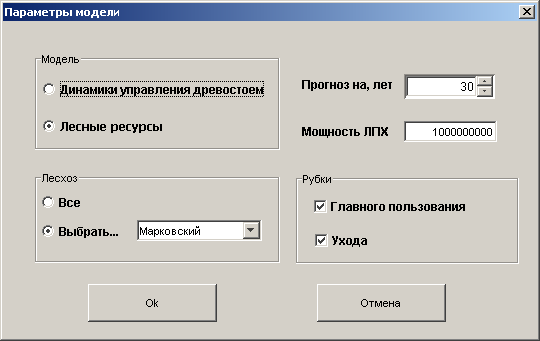
\includegraphics[width=405pt, height=256pt, keepaspectratio=true]{asyaDisser9_3-fig002.png}
%%\caption{This should be the caption for \texttt{asyaDisser9\_3-fig002.png}.}
%%\end{figure}

Рис. 3.3. Задание базовых параметров задачи 
\end{center}

Подсистема искусственного интеллекта позволяет 
автоматизировать процесс построения математической 
модели природного объекта на этапах идентификации 
параметров модели по исходным данным об объекте, 
синтеза структуры модели. В настоящее время 
база моделей информационной системы содержит 
модели ДУД и «Лесные ресурсы». Подсистема искусственного 
интеллекта реализована на основе базы знаний, 
содержащей знания о базовой структуре каждой 
модели, об идентификации модели на основе данных 
об исследуемом объекте, а также поиска начальных 
условий модели. 

Исходные данные для идентификации модели и 
вычисления начальных условий загружаются из 
различных источников данных, которыми, как 
правило, выступают базы данных. Запросы к базам 
данных генерируются подпрограммами, запускаемыми 
механизмом логического вывода в процессе построения 
формализованного представления модели конкретного 
исследуемого объекта. 

После импорта данных интерфейсным модулем 
программы производятся расчеты по модели, при 
этом предварительно выбирается один из вариантов 
стратегии управления лесными ресурсами (естественная 
или антропогенная динамика). 

В режиме моделирования с использованием антропогенной 
динамики пользователь имеет возможность задавать 
управляющее воздействие (параметры рубок). 
Смена характера развития моделируемой природной 
системы отражается величиной коэффициентов 
модели, связанных со скоростью процессов возобновления 
и роста деревьев. Правила базы знаний позволяют 
гибко определять такие антропогенные воздействия 
на ЛР как объемы рубок, насаждений в зависимости 
от набора параметров. Например, объем рубок 
изменяется на каждом шаге интервала прогнозирования 
отдельно для каждого моделируемого участка, 
в зависимости от расчетных данных.

При расчетах по математическим моделям в той 
или иной мере используются пространственно-распределенные 
данные, что требует обеспечения тесного взаимодействия 
с современными ГИС, используемыми, в частности, 
для представления результатов прогнозных расчетов 
в виде цифровых карт. Автоматическое картографирование 
промежуточных стадий вычислений по моделям 
позволяет исследователю контролировать процесс 
моделирования.

\begin{center}
начало
База знаний

Ввод параметров задачи

Расчеты по модели

Многокритериальная оптимизация

Отображение данных расчетов

конецБаза данных

Идентификация модели

Формирование сценариев

Сохранение данных

Создание графиков

Создание карт, анимации

Рис. 3.4. Технологическая схема автоматизации 
моделирования.
\end{center}

Комбинации значений параметров отображают 
управляющее воздействие на объект (гипотетическое 
решение ЛПР). В последнюю очередь определяются 
критерии\textit{ }анализа получаемых результатов 
прогнозных расчетов (расчета сценариев). Критерии 
свёртывают расчеты к набору числовых характеристик, 
которые идентифицируют сценарий и задают его 
положение в пространстве\textit{ }критериев. Заключительным 
этапом анализа модельных расчетов является 
многокритериальная оптимизация.

Полученные в результате расчета данные, например, 
в модели ДУД - распределение площадей по породам 
и классам возраста, а также и по времени, формируют 
базу данных формата CSV, и по запросу пользователя 
отображаются виде графиков, карт и  картографических 
анимаций (рис. 3.4).\label{HToc128995781}\label{HToc199746727}

\subsubsection*{\textbf{3.3. Структура информационной системы}}

Информационная системы разрабатывается на 
основе программной технологии Java, которая является 
объектно-ориентированной,  платформо-независимой 
[79, 84]. Байт-код, который получается после компиляции 
Java-программы, может интерпретироваться на любой 
платформе, где установлена виртуальная машина 
Java. Java обеспечивает динамическую сборку программы. 
Классы подгружаются по мере необходимости, 
причем загружены они могут быть не только  локального 
компьютера, но и с любой точки сети Интернет. 
Также Java обладает встроенной поддержкой сетевых 
технологий (как локальных, так и Internet/Intranet), 
возможности переносимости программ между программно-аппаратными 
платформами, мощными стандартными библиотеками. 
Кроме того, java-приложения, реализованные специальным 
образом, встраиваются в HTML страницу в виде так 
называемого апплета (applet). При этом апплет является 
программой, т.е. он реагирует на действия пользователя, 
получает от него исходные данные, производит 
расчеты, выдает результаты.

Использование технологии Java при разработке 
информационной системы позволило использовать 
возможности имеющихся java-библиотек (например, 
для работы с картами, обработки Пролога), реализовать 
управление отдельными модулями информационной 
системы с помощью скриптов на основе JavaScript, 
создать вариант информационной системы в виде 
апплета.

\textit{\textbf{Графическая подсистема}}

\textit{\textbf{Подсистема искусственного интеллекта}}

\textit{\textbf{Подсистема математического моделирования}}

\begin{center}
Базы данных

База 

знанийБаза моделей\fancyfoot[LE]{\thepage{}}
\fancyfoot[LO]{\thepage{}}

Рис. 3.5. Информационные потоки ИС
\end{center}

Информационные потоки ИС приведены на рис. 
3.5. Подсистема математического моделирования 
представлена блоком численных расчетов, базой 
данных и моделей; подсистема искусственного 
интеллекта - блоками параметрической идентификации, 
запросной подсистемой, базой знаний; графическая 
подсистема - блоками ГИС, визуализации результатов. 
Интерфейсная подсистема взаимодействует со 
всеми этими подсистемами, передавая данные 
по запросам пользователей.

Все подсистемы реализованы в виде модулей информационной 
системы (рис. 3.6). В модуле \textit{Calculate} производятся 
численные расчеты по моделям, отправляются 
запросы к БЗ, модуль \textit{jsCalc} осуществляет взаимодействие 
между ИС и пользовательскими приложениями 
на \textit{JavaScript}. Модуль \textit{SimpleMap} создает карты 
и анимации, модуль \textit{Diagr} - диаграммы. В модуле 
\textit{lesvar} хранятся константы для расчетов по 
моделям, модули \textit{main, ScenarPr, MapParam, DiagrParam} содержат 
набор пользовательских форм и образуют подсистему 
пользовательского интерфейса.

%%\begin{figure}[htbp]
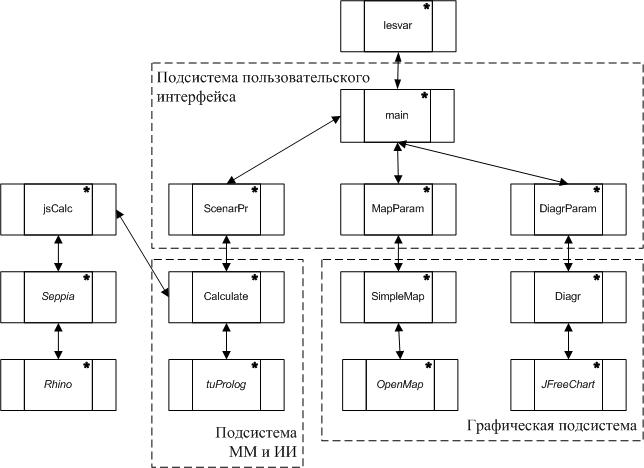
\includegraphics[width=449pt, height=326pt, keepaspectratio=true]{asyaDisser9_3-fig003.png}
%%\caption{This should be the caption for \texttt{asyaDisser9\_3-fig003.png}.}
%%\end{figure}

\begin{center}
Рис. 3.6. Модульная структура информационной 
системы
\end{center}

На рисунке курсивом обозначены используемые 
 сторонние библиотеки (\textit{JFreeChart, OpenMap, tuProlog, 
Rhino, Seppia}).\label{HToc199746728}

\textbf{3.3.1. Информационное обеспечение системы 
}

Исходной информацией служат данные учета лесного 
фонда, которые представляют собой таблицы распределения 
площадей и запасов лесов по преобладающим породам 
и группам возраста. Основным источником информации 
о направлениях смены пород и возрастных циклах 
древостоев на всей территории лесхоза являются 
научные публикации, отражающие закономерности 
динамики леса в различных регионах. Эти обширные 
материалы составляют информационную основу 
подсистемы математического моделирования.

Данные для модели ДУД по Иркутской области 
содержат информацию по таким породам как сосна, 
ель, пихта, лиственница, кедр, береза, осина, 
а также в целом по хвойным и мягколиственным 
породам. В свою очередь они подразделяются 
на данные по группам возраста: молодняки 1 и 
2 класса, средневозрастные, приспевающие, спелые 
и перестойные. Также для расчетов используются 
данные о площади лесхоза, количестве населения, 
проживающего на территории лесхоза. Такие данные 
существуют по 53 из 59 лесхозов, имеющихся в Иркутской 
области.

Данные предоставлены Институтом географии 
СО РАН, по состоянию на 1 января 2004 г., по формам, 
утвержденным Рослехозом, в текстовых файлах 
формата *.txt. При передаче в информационную систему 
данные преобразованы в БД формата Microsoft Excel.

Эти данные используются для определения начальных 
и граничных условий решения дифференциальных 
уравнений модели ДУД, оценки комплексных характеристик 
состояния условий природной среды и вычисления 
ряда коэффициентов.

Для определения интенсивности рубок ухода 
и главного пользования использовались Правила 
рубок главного пользования в лесах Восточной 
Сибири [70] и Наставления по рубкам ухода в лесах 
Восточной Сибири [61]. Эти правила определяют 
порядок проведения рубок, их объемы, в зависимости 
от породы, класса возраста, распределения лесов 
по зонам и подзонам, крутизны склонов.

Данные для модели «Лесные ресурсы» взяты из 
БД ГИС поквартальных итогов, формат данных 
- *.dbf. В материалах поквартальных итогов содержится 
информация о распределении площади квартала 
по категориям земель, площади и запасов лесов 
по породам и группам возраста, о средних таксационных 
характеристиках (табл. 1). В таблице 1 в столбце 
«Тип» значение «С» соответствует символьным 
данным, «Ц» - числовым. 

\begin{flushright}
Таблица 1. Структура базы данных поквартальных 
итогов 

\begin{tabular}{|>{\raggedright}p{71pt}|>{\raggedright}p{200pt}|>{\raggedright}p{58pt}|>{\raggedright}p{22pt}|>{\raggedright}p{51pt}|}
\hline
П\textbf{оле в БД} & Н\textbf{аименование} & Е\textbf{диница 
измерения} & Т\textbf{ип} & К\textbf{оличество}\linebreak{}
\textbf{знаков}\tabularnewline
\hline
Region & Название области &  & С & 32\tabularnewline
\hline
Cod\_Region & Код области &  & Ц & 10\tabularnewline
\hline
Raion & Название района &  & С & 32\tabularnewline
\hline
Code\_Raion & Код района &  & Ц & 5\tabularnewline
\hline
Leshoz & Название лесхоза &  & С & 32\tabularnewline
\hline
Cod\_Leshoz & Код лесхоза &  & Ц & 8\tabularnewline
\hline
Lesnich & Название лесничества &  & С & 32\tabularnewline
\hline
Code\_Lesn & Код лесничества &  & Ц & 10\tabularnewline
\hline
Kvartal & Номер квартала &  & Ц & 4\tabularnewline
\hline
Zaschit-t & Категория защитности &  & C & 32\tabularnewline
\hline
ID & ГИС-идентификатор &  & Ц & 16\tabularnewline
\hline
Landscape & Тип ландшафта &  & С & 32\tabularnewline
\hline
Prb\_S\_kind & Преобладающая по площади порода &  & С & 32\tabularnewline
\hline
Prb\_W\_kind & Преобладающая по запасу порода &  & С & 32\tabularnewline
\hline
Prb\_S\_GrVz & Преобладающая по площади группа возраста &  & С & 32\tabularnewline
\hline
Prb\_S\_Type & Преобладающий по площади тип леса &  & С & 32\tabularnewline
\hline
S\_Lzem & Площадь лесных земель & Га & Ц & 5\tabularnewline
\hline
S\_L & Площадь покрытых лесом & Га & Ц & 5\tabularnewline
\hline
S\_SLk & Площадь сомкнувшихся лесных культур & Га & Ц & 5\tabularnewline
\hline
S\_NLk & Площадь несомкнувшихся лесных культур & Га & Ц & 5\tabularnewline
\hline
S\_LP & Площадь лесных питомников & Га & Ц & 5\tabularnewline
\hline
S\_redin & Площадь редин & Га & Ц & 5\tabularnewline
\hline
S\_fire & Площадь гарей, погибших насаждений & Га & Ц & 5\tabularnewline
\hline
S\_cut & Площадь вырубок & Га & Ц & 5\tabularnewline
\hline
S\_glade & Площадь прогалин, пустырей & Га & Ц & 5\tabularnewline
\hline
S\_N & Площадь непокрытых лесом земель & Га & Ц & 5\tabularnewline
\hline
S\_forest & Площадь лесных земель & Га & Ц & 5\tabularnewline
\hline
S\_arable & Площадь пашен & Га & Ц & 5\tabularnewline
\hline
S\_hay & Площадь сенокосов & Га & Ц & 5\tabularnewline
\hline
S\_pasture & Площадь пастбищ & Га & Ц & 5\tabularnewline
\hline
S\_water & Площадь вод & Га & Ц & 5\tabularnewline
\hline
S\_road & Площадь дорог и просек & Га & Ц & 5\tabularnewline
\hline
S\_house & Площадь усадеб и пр. земель & Га & Ц & 5\tabularnewline
\hline
S\_bog & Площадь болот & Га & Ц & 5\tabularnewline
\hline
S\_other & Прочие земли & Га & Ц & 5\tabularnewline
\hline
S\_noforest & Площадь лесных земель & Га & Ц & 5\tabularnewline
\hline
W\_All & Общий запас насаждения & Дес. м\textsuperscript{3} & Ц & 7\tabularnewline
\hline
W\_redin & Запас редин & Дес. м\textsuperscript{3} & Ц & 5\tabularnewline
\hline
W\_ones & Запас единичн. деревьев & Дес. м\textsuperscript{3} & Ц & 5\tabularnewline
\hline
W\_growth & Запас сырорастущего & Дес. м\textsuperscript{3} & Ц & 7\tabularnewline
\hline
W\_new\_dry & Запас свежего сухостоя & Дес. м\textsuperscript{3} & Ц & 5\tabularnewline
\hline
W\_dry & Запас сухостоя & Дес. м\textsuperscript{3} & Ц & 5\tabularnewline
\hline
Stuff & Захламленность & Дес. м\textsuperscript{3} & Ц & 5\tabularnewline
\hline
Stuff\_Likv & Захламленность ликвида & Дес. м\textsuperscript{3} & Ц & 5\tabularnewline
\hline
S\_Pris & Площадь приспевающих & Га & Ц & 5\tabularnewline
\hline
W\_Pris & Запас приспевающих & Дес. м\textsuperscript{3} & Ц & 5\tabularnewline
\hline
CenterX & Координата центра квартала по x &  & Ц & 5\tabularnewline
\hline
CenterY & Координата центра квартала по y &  & Ц & 5\tabularnewline
\hline
\end{tabular}
\end{flushright}

Данные поквартальных итогов описанной выше 
структуры содержат достаточно информации для 
информационного обеспечения математической 
модели «Лесные ресурсы». БД квартальной сети 
позволяет вместо регулярной сетки интегрирования 
использовать в качестве основы дискретизации 
пространства квартальную нерегулярную сеть. 
Практически это не слишком осложняет вычисления, 
но позволяет результаты расчетов использовать 
в том же режиме, что и исходные данные, визуализировать 
их как обычные базы данных поквартальных итогов. 

Для определения удаленности квартала от вектора 
направления рубки в имеющуюся БД добавлены 
поля CenterX и CenterY (табл. 1), являющиеся координатами 
центра квартала. Их значения рассчитаны с помощью 
ГИС ArcView 3.2.

В БД ГИС входит цифровая топографическая основа 
Иркутской области (для модели ДУД) и Усть-Илимского 
района (для модели «Лесные ресурсы»).

Данные расчетов сохраняются в БД формата Microsoft 
Excel (в формате *.csv). Формат CSV является текстовым 
форматом, предназначенным для представления 
табличных данных. Каждая строка файла - это 
одна строка таблицы, а значения отдельных колонок 
разделяются символом-разделителем, например, 
запятой или точкой с запятой. Редактировать 
файлы такого формата пользователь может как 
с помощью программы Microsoft Excel, так и с помощью 
любого текстового редактора.

Для модели ДУД структура сохраненных данных 
имеет следующий вид:

\ensuremath{-} Номер лесхоза

\S{} Наименование породы

1. Год,

2. Общая лесная площадь,

3. Площадь молодняков 1 кл.,

4. Площадь молодняков 2 кл.,

5. Площадь средневозрастных,

6. Площадь приспевающих,

7. Площадь спелых и перестойных.

Для модели «Лесные ресурсы» данные сохраняются 
в формате:

\ensuremath{-} Номер квартала

1. Год,

2. Общая лесная площадь,

3. Площадь молодняков и средневозрастных,

4. Площадь приспевающих,

5. Площадь спелых и перестойных.\label{HToc199746729}

\textbf{3.3.2. Представление моделей лесных ресурсов}

В модуле \textit{lesvar} (рис. 3.3) содержится набор констант, 
используемых при расчетах динамики лесных 
ресурсов. Это массивы \textit{lesh[]} - перечень лесхозов 
Иркутской области, \textit{type[]} - породы леса, \textit{vozr[]} 
- категории земель и классы возраста.

Размерности \textit{L,P,V} массива \textit{Si[L][T][P][V]}, используемого 
для расчетов по модели ДУД, задаются согласно 
размерности соответствующих массивов-констант 
модуля \textit{lesvar}, а размерность \textit{T} - в зависимости 
от количества лет интервала моделирования, 
заданного пользователем.

При расчетах по модели «Лесные ресурсы» у массива 
\textit{Slr[T][N][V]} размерность \textit{V} соответствует 
количеству категорий земель и классов возраста, 
\textit{N} - количество записей (кварталов) в исходной 
БД, \textit{T} - задается пользователем.\label{HToc199746730}

\textbf{3.3.3. Реализация моделей лесных ресурсов}

Расчеты по моделям ДУД и «Лесные ресурсы» производятся 
соответственно процедурам \textit{DUD()} и \textit{LesRes()}. 

Для модели \textbf{ДУД} алгоритм расчетов выглядит 
следующим образом:

1) с помощью базы знаний строится матрица коэффициентов 
\textit{a}\textsubscript{\textit{ij}}\textit{ }(\textit{i(unknown char)1..N, j(unknown char)1..N, 
N} - количество классов возраста) интенсивности 
перехода участков леса из одного состояния 
в другое;

2) если выбрано проведение рубок ухода и/или 
главного пользования, то из БЗ определяется 
их интенсивность для каждой породы и каждого 
класса возраста и заполняются массивы \textit{Uh}\textsubscript{\textit{ij 
}}и\textit{ Ur}\textsubscript{\textit{ij}}\textit{ }(\textit{i(unknown char)1..M, 
j(unknown char)1..N, M} - количество пород, \textit{N} - количество 
классов возраста)\textit{;}

3) из БД извлекаются данные в целом по лесхозу: 
полная площадь \textit{S}, не покрытая лесом площадь 
\textit{Snp}, количество населения \textit{Nas};

4) из БД извлекаются начальные данные распределения 
площадей по породам и классам возраста \textit{Si[L][T][P][V] 
}(\textit{L} - количество лесхозов\textit{,T} - количество 
лет в интервале моделирования\textit{,P} - количество 
пород\textit{,V} - количество классов возраста);

5) рассчитываются начальные и граничные условия;

6) по годам от 1 до \textit{T}:

1) проводятся численные расчеты по модели методом 
Рунге-Кутта;

2) определяется управление: рубки ухода, рубки 
главного пользования, пожары, лесопосадки;

3) вычисляются критерии оценки результата.

Если выбрано проведение расчетов для ряда лесхозов, 
то шаги 3-6 повторяются для каждого из них.

Для модели \textbf{«Лесные ресурсы»} алгоритм расчетов 
выглядит следующим образом:

1) с помощью JDBC из БД извлекаются начальные данные 
по каждому из кварталов \textit{Slr[T][N][V]} (\textit{T} - 
количество лет в интервале моделирования, \textit{N} 
- количество кварталов, \textit{V} - количество классов 
возраста);

2) определяются параметры вектора рубки \textit{VecR(x0, 
y0, x1, y1)};

3) по годам от 1 до \textit{T}:

1) проводятся численные расчеты естественной 
динамики;

2) рассчитывается вырубка;

3) определяется увеличение нелесной площади 
\textit{Un}\textsubscript{\textit{i}};

4) вычисляются критерии оценки результата.\label{HToc199746731}

\textbf{3.3.4. Реализация численных расчетов}

Модели динамки лесных ресурсов содержат в своей 
структуре как обыкновенные дифференциальные 
уравнения, так и уравнения с частными производными. 
Для их численного решения применяются методы 
Рунге-Кутта и разностных схем. Эти методы основаны 
на введение некоторой разностной сетки в рассматриваемой 
области. Значений производных, начальные и 
граничные условия выражаются через значения 
функций в узлах сетки, в результате чего получается 
система алгебраических уравнений, называемая 
разностной схемой. Решая эту систему уравнений, 
можно найти в узлах сетки значения сточных 
функций, которые приближенно считаются равными 
значениям искомых функций [42, 80].\label{HToc199746732}

\textbf{3.3.5. База знаний}

Для задачи автоматизации идентификации модели 
в базе знаний определены следующие входные 
данные:

1) характеристики исследуемого объекта (термы\textit{ 
}ранг геосистемы \textit{rang()}, тип ландшафта \textit{type\_land()});

2) формулировка решаемой задачи, например, моделирование 
динамики, расчеты вырубок, пожаров и т.п.  (термы 
\textit{problem()});

3) виды пород леса (термы \textit{porod()});

4) характеристики смены классов возраста в процессе 
роста леса (термы \textit{smena()});

5) характеристики интенсивности смены классов 
возраста в процессе роста леса (термы \textit{intens()});

6) виды пород леса, вырубаемых на рассматриваемой 
территории (терм \textit{porodRub( )});

7) типы классов возраста леса (термы \textit{vozrast()});

8) классы возраста леса, который можно вырубать 
(термы \textit{rubkaGP\_type()});

9) характеристики рубок главного пользования 
(термы \textit{rubGP()});

10) характеристики рубок ухода (термы \textit{rubUh()});

11) характеристики начального состояния объекта 
моделирования (термы \textit{s0()});

12) характеристики начального состояния объекта 
моделирования  по породе и классу возраста 
(термы \textit{sq()}).

Запросы к структуре моделей и расчетным данным, 
поддержка логического вывода в процессе идентификации 
моделей осуществляются с помощью правил базы 
знаний.

Для получения данных о состоянии объекта моделирования 
в начальный момент времени \textit{t}\textsubscript{\textit{0}} 
для модели ДУД используется правило:

\begin{center}
\textit{fs0(model(dud), Lesh, S, Snep, Nas) :- s0(Lesh, t0, S, Snep, Nas).}
\end{center}

Результатом работы правила будут общая площадь 
\textit{S}, не покрытая площадь \textit{Snep} и численность 
населения \textit{Nas} для лесхоза \textit{Lesh}.

Исходные данные о площадях, занятых породой 
определенного класса возраста получаются с 
помощью правил вида:

\begin{center}
\textit{square(Lesh, Prd, vozrast(\texttt{"}молодняки 1кл \texttt{"}), 
t0, S) :-}

\textit{:- sq(Lesh, Prd, \_, S,\_, \_, \_, \_).}
\end{center}

Структура типа \textit{sq(Lesh, Prd, S, Sm1, Sm2, Ssr, Spr, Ssp) }содержит 
данные о площадях лесхоза \textit{Lesh} породы \textit{Prd:} 
общей \textit{S}, молодняков 1 кл. \textit{Sm1} и 2 кл \textit{Sm2}, 
средневозрастных \textit{Ssr}, приспевающих \textit{Spr}, 
спелых и перестойных \textit{Ssp}.

Для построения последовательности смены участками 
леса своих возрастных классов в модели ДУД 
применяется правило:

\begin{center}
\textit{perehod(model(dud), Prd, Kl, Kl2, In) :- smena(Kl2, Kl), intens(Prd, In).}
\end{center}

«В модели ДУД переход леса породы \textit{Prd} из 
класса \textit{Kl} в класс \textit{Kl2} с интенсивностью\textit{ 
In }осуществляется, если \textit{Kl2 }сменяет \textit{Kl} 
и интенсивность для породы \textit{Prd} равна \textit{In}».

Рубки ухода определяются правилом:

\begin{center}
\textit{rubUh(porod(K), vozrast(V), X) :- rubUh(K, V, X).}
\end{center}

Правило проведения рубок главного пользования 
выглядит следующим образом:

\begin{center}
\textit{rubkaGP(model(dud), porod(K), vozrast(V), Vr) :-         }

\textit{:-porodRub(K), rubkaGP\_type(V), rubGP(K, Vr).}
\end{center}

«В модели ДУД рубки главного пользования по 
породе \textit{K} возраста \textit{V} объемом \textit{Vr} 
проводятся, если порода \textit{K} может вырубаться, 
ее возраст \textit{V} подлежит вырубке и объем ее 
рубки составляет\textit{ Vr}».\label{HToc199746733}

\textbf{3.3.6. Подсистема отображения результатов 
расчетов}

Режим интерактивного задания критериев анализа 
результатов расчетов предназначен для пользователей 
с низкой квалификацией программиста. Для основного 
режима задания критериев разработаны специализированные 
пользовательские интерфейсы, со встроенными 
элементами управления, позволяющие выбрать 
определенные показатели. В этом режиме предоставляется 
интерактивный механизм формирования пользовательских 
аналитических процедур (рис. 3.7). Он позволяет 
задавать множество переменных, соответствующих 
временным рядам исследуемого природного процесса, 
и действия над этими переменными.

\begin{center}
%%\begin{figure}[htbp]
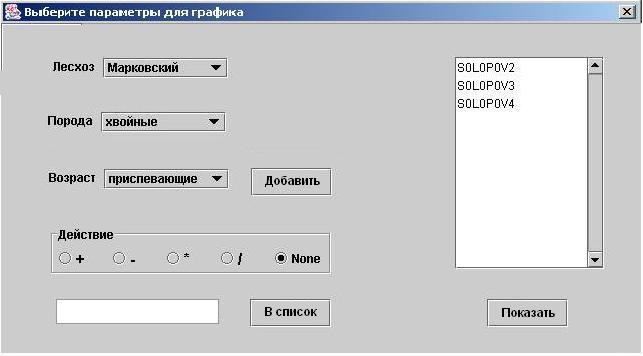
\includegraphics[width=453pt, height=251pt, keepaspectratio=true]{asyaDisser9_3-fig004.jpg}
%%\caption{This should be the caption for \texttt{asyaDisser9\_3-fig004.jpg}.}
%%\end{figure}

Рис. 3.7. Выбор параметров графика
\end{center}

Пользователь сначала выбирает временной ряд, 
затем, если необходимо, одну из математических 
операций (сложение, вычитание, умножение, деление), 
другой временной ряд и так далее. Получившееся 
выражение добавляется к списку. Когда список 
готов, можно увидеть запрошенный график (рис. 
3.8).

Такой механизм позволяет пользователям формировать 
порядка 50\% базовых аналитических процедур, 
при этом набор операций ограничен элементарными 
арифметическими операциями и выборками временных 
рядов.

%%\begin{figure}[htbp]
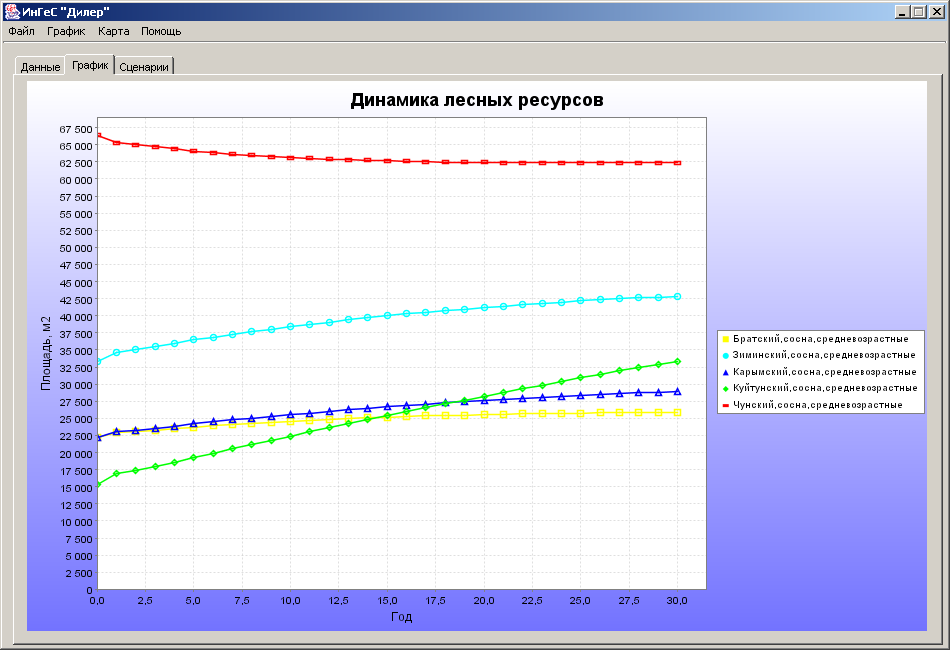
\includegraphics[width=463pt, height=317pt, keepaspectratio=true]{asyaDisser9_3-fig005.png}
%%\caption{This should be the caption for \texttt{asyaDisser9\_3-fig005.png}.}
%%\end{figure}

\begin{center}
Рис 3.8. Полученный график
\end{center}

Интерактивный режим позволяет быстро увидеть 
полученные результаты. Однако в нем может быть 
сформировано только ограниченное число разновидностей 
критериев, на основе тех операций, которые внесены 
в систему при разработке.

Для отрисовки графиков используется библиотека 
\textit{JFreeChart}. \textit{JFreeChart} - свободно распространяемая 
Java-библиотека, она позволяет создавать различные 
виды графиков и диаграмм, например, гистограммы, 
круговые диаграммы, временные ряды и т.д. При 
необходимости готовый графический материал 
сохраняется в формате JPEG.

После выбора временных рядов, которые необходимо 
отобразить на графике, класс \textit{DiagrParam()} обращается 
к процедуре \textit{Diagr(String[] labels, Vector ar)} класса \textit{Diagr()}. 
Параметрами процедуры являются массив строк-подписей 
к графикам и набор прогнозных расчетных данные 
типа Vector. Vector - тип, позволяющие хранить разнообразные 
данные (строковые, числовые), причем его элементы 
также могут иметь тип Vector. В блоке построения 
графиков устанавливаются заголовок графика, 
подписи под осями координат, цвет и тип линии 
каждого временного ряда.\label{HToc199746734}

\textbf{3.3.7. Формирование сценариев}

При проведении расчетов по моделям пользователю 
доступны для изменения следующие параметры: 
объем рубок ухода, рубок главного пользования, 
пожаров и лесопосадок. Каждый из этих параметров 
может принимать значения от 0\% (отсутствие) 
до 100\% (полный объем).

\begin{center}
%%\begin{figure}[htbp]
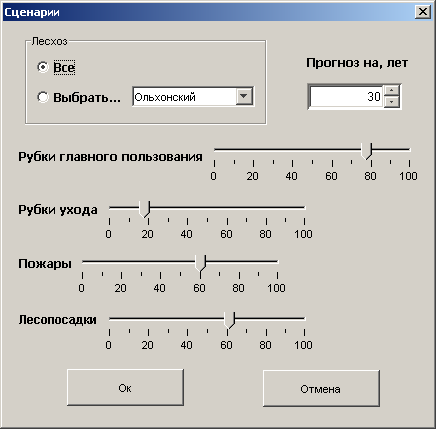
\includegraphics[width=252pt, height=248pt, keepaspectratio=true]{asyaDisser9_3-fig006.png}
%%\caption{This should be the caption for \texttt{asyaDisser9\_3-fig006.png}.}
%%\end{figure}

Рис. 3.9. Формирование сценариев расчета
\end{center}

В информационной системе для ДУД задан следующий 
набор критериев:

1. $\max  _{j} \min  _{i} V_{b}^{j} (t_{i} ) $ , где V\textsuperscript{j}\textsubscript{b}(t\textsubscript{i}) 
- объем биомассы (по всем породам и возрастам), 
рассчитанный по j-му сценарию в году t\textsubscript{i};

2. $\min  _{j} \max  _{i} S_{g}^{j} (t_{i} ) $ , где S\textsuperscript{j}\textsubscript{g}(t\textsubscript{i}) 
- площадь «непокрытая лесом», рассчитанная 
по j-му сценарию в году t\textsubscript{i}, на которой 
лес может произрастать;

3. $\max  _{j} \left( S_{p}^{j} +S_{s}^{j} \right)  $ , где S\textsuperscript{j}\textsubscript{p}, 
S\textsuperscript{j}\textsubscript{s} - соответственно площадь 
перестойных и спелых лесов (запас деловой древесины), 
рассчитанная по j-му сценарию за прогнозируемый 
период;

4. $\max  _{j} V_{x}^{j}  $ , где V\textsuperscript{j}\textsubscript{r } - суммарный 
объем рубок, рассчитанный по j-му сценарию за 
прогнозируемый период.

Каждый расчетный сценарий оценивается по данному 
набору критериев, из полученного множества 
альтернатив выделяется множество парето-оптимальных 
решений.

%%\begin{figure}[htbp]
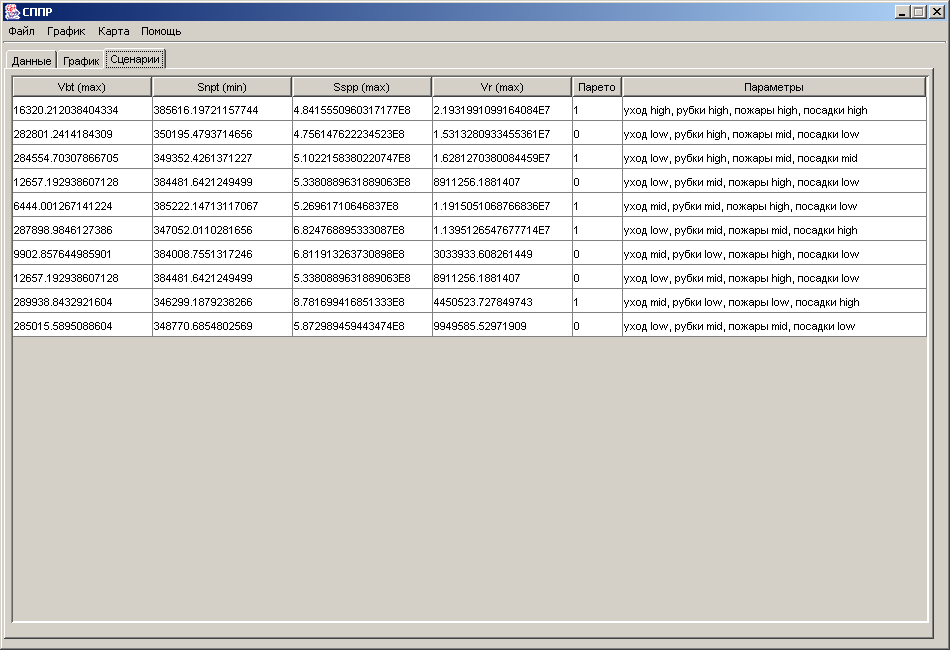
\includegraphics[width=463pt, height=317pt, keepaspectratio=true]{asyaDisser9_3-fig007.png}
%%\caption{This should be the caption for \texttt{asyaDisser9\_3-fig007.png}.}
%%\end{figure}

\begin{center}
Рис. 3.10. Результаты оптимизации набора сценариев
\end{center}

На рис. 3.10 приведены результаты расчетов по 
сценариям по всем лесхозам Иркутской области 
по модели ДУД. В таблице содержатся значения 
критериев по каждому сценарию, параметры сценариев. 
После расчета прогнозов проведена оптимизация 
- выделение множества парето-оптимальных решений. 

В модели «Лесные ресурсы» эффективность выбранной 
стратегии рубки оценивается по двум критериям:

1. объему заготовленной древесины за время \textit{Т} 
(unknown char) 100 лет:
$$I_{W} =k\sum\limits_{j=1}^{3}\iiint\limits_{\text{T   S} } w_{j} \left( \xi _{1} \right) u_{j} \left( t,\xi _{1} \right)  dtd\xi _{1}   $$
                           \begin{flushright}
(3.1)
\end{flushright}

2. степени выполнения лесами района средообразующих 
функций за то же время \textit{Т}:
$$I_{Q} =k\sum\limits_{j=1}^{3}\iiint\limits_{\text{T S} _{\text{III} } } q_{j} S_{j} \left( t,\xi _{1} \right)  dtd\xi _{1}  ,\eqno(3.2) $$
\label{OLEHLINK14}\label{OLEHLINK15}где \textit{k (unknown char)} 0,75 --- коэффициент 
выхода деловой древесины;

\textit{q}\textsubscript{\textit{j}}\textit{ ---} оценка невесомой 
функции леса, например его водорегулирующей 
роли, для соответствующих категорий земель 
и групп возраста.

Значения \textit{q}\textsubscript{\textit{j}} определяются 
путем экспертных оценок, причем за единицу 
принята \textit{q}\textsubscript{2}\textit{ }для приспевающих 
древостоев. Для молодняков и средневозрастных 
древостоев \textit{q}\textsubscript{\textit{j}}  (unknown char) 0,5, 
спелых и перестойных насаждений --- 0,95, нелесной 
площади --- 0,3, не покрытой лесом площади --- 0,4.\label{HToc199746735}

\textbf{3.3.8. Сетевой доступ к информационной системе}

В настоящее время развиваются технологии, позволяющие 
получить доступ к программам и прикладным пакетам 
через протокол http. При этом ИС находится не 
на компьютере пользователя, а на удаленном 
компьютере - сервере. Данный подход удобен тем, 
что для проведения расчетов достаточно обладать 
доступом в сеть Интернет и программой-браузером. 
Это позволяет обеспечить доступ к информационной 
системе большему количеству исследователей, 
не требовать установки дополнительного программного 
обеспечения на компьютер пользователя (только 
Браузер и plug-in Java-машины), централизованно управлять 
серверным приложением информационной системы.

В качестве базовой технологии отображения 
информации выбран подход, базирующийся на встраивании 
интерфейса пользователя Java-приложения в современные 
Интернет-браузеры, так называемые апплеты. 
На сервере хранится файл-архив типа *.jar, в котором 
содержатся исходные данные для расчетов по 
модели, модули информационной системы. Запуск 
апплета происходит из файла FR.html (рис. 3.11). 

Перед началом расчетов пользователь выбирает 
тип модели, тип динамики лесных ресурсов (естественная 
или антропогенная), породу и интервал моделирования. 
Результаты выдаются в табличном виде и могут 
быть сохранены в формате Microsoft Excel.

%%\begin{figure}[htbp]
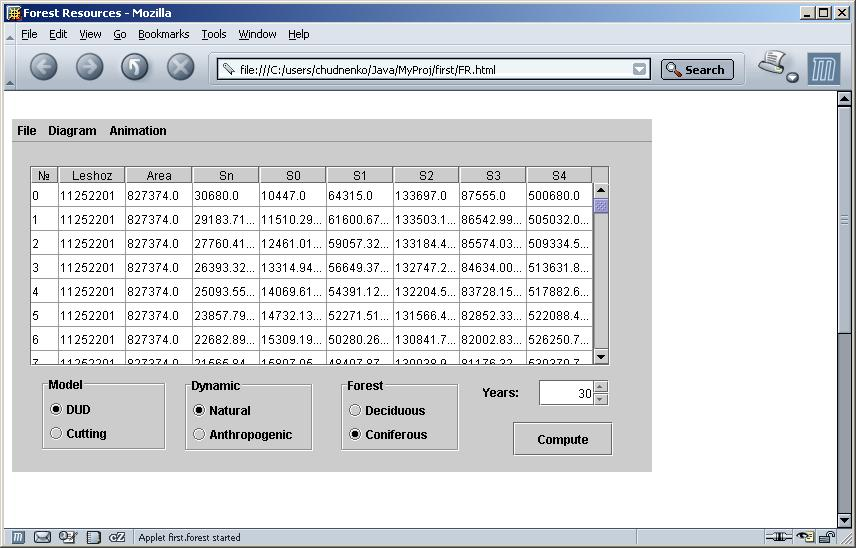
\includegraphics[width=454pt, height=291pt, keepaspectratio=true]{asyaDisser9_3-fig008.jpg}
%%\caption{This should be the caption for \texttt{asyaDisser9\_3-fig008.jpg}.}
%%\end{figure}

\begin{center}
Рис. 3.11. Представление  информационной системы 
в виде апплета 
\end{center}

Апплет является доверенным (trusted), что позволяет 
ему сохранять данные на компьютер пользователя, 
т.к. для обычных апплетов действия с компьютерами 
пользователей запрещены для обеспечения их 
безопасности. Поэтому перед запуском доверенного 
апплета выдается сообщение, в котором указываются 
параметры апплета (кем и для чего был он создан) 
и запрашивается подтверждение на его использование.

По результатам расчетов по запросу пользователя 
строятся графики и диаграммы, также апплет 
позволяет отображать площадную информацию 
по прогнозным расчетам на карте (рис. 3.12). 

Элементы управления апплета позволяют выполнять 
следующие функции:

\ensuremath{-} перемещать центр изображения (Панорамирование);

\ensuremath{-} изменять масштаб изображения (Наезд);

\ensuremath{-} изменять набор отображаемых слоев;

\ensuremath{-} изменять режимы просмотра изображения;

\ensuremath{-} осуществлять запросы к объектам картографического 
произведения.

\begin{center}
%%\begin{figure}[htbp]
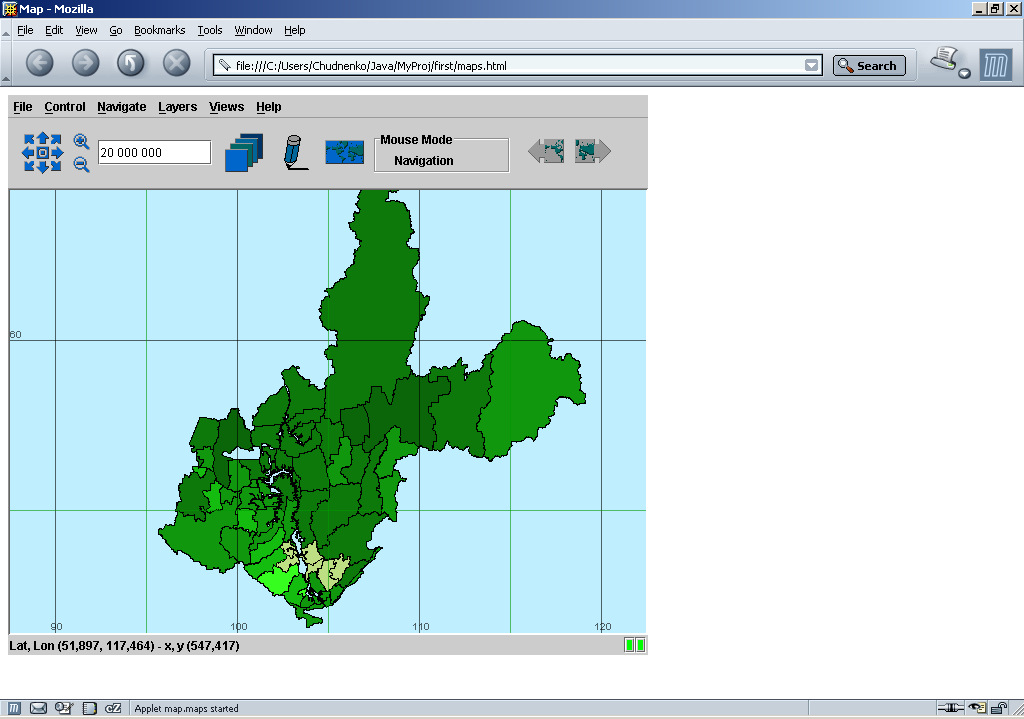
\includegraphics[width=445pt, height=313pt, keepaspectratio=true]{asyaDisser9_3-fig009.png}
%%\caption{This should be the caption for \texttt{asyaDisser9\_3-fig009.png}.}
%%\end{figure}

Рис. 3.12. Отображение в апплете расчетных данных\label{HToc199746736}
\end{center}

\subsubsection*{\textbf{3.4. Инструментальные средства 
информационной системы\label{HToc199746737}}}

\textbf{3.4.1. Средства программирования пользовательских 
приложений}

Базовые блоки информационной системы позволяют 
рассчитывать динамику лесных ресурсов. Описание 
задачи прогнозирования, объекта моделирования, 
задание сценариев проведения расчетов производится 
в процессе диалога пользователя с информационной 
системой. Однако при решении некоторых задач 
пользователю может потребоваться расширение 
возможностей ИС. Для этого в состав информационной 
системы включены инструментальные средства, 
позволяющие пользователям создавать на ее 
основе специализированные приложения.

Данные средства призваны обеспечить пользователя 
возможностью самому управлять функционированием 
программы, изменяя некоторые  модули. При этом 
изменяемые модули создаются на языках, программирование 
на которых не требует наличия специальной программной 
среды. С помощью таких инструментальных средств 
можно решать, например, задачу задания дополнительных 
критериев анализа результатов, полученных 
в ходе расчетов информационной системы. Поэтому 
в ИС включены два режима задания критериев 
анализа результатов расчетов: интерактивный 
(п. 3.3.6) и механизм программирования пользовательских 
приложений.\label{OLEHLINK8}\label{OLEHLINK9}

Средства программирования пользовательских 
приложений реализованы при помощи интерпретатора 
языка программирования JavaScript и специальной 
библиотеки jsCalc, что позволяет интегрировать 
множество базовых функций и объектов в рамках 
одного приложения. Библиотека реализована 
в виде модуля информационной системы, она предоставляет 
доступ к различным функциям программы, например, 
построению графиков, карт. Процедуры  библиотеки 
jsCalc  вызываются непосредственно скриптом на 
языке JavaScript. В программу-приложение JavaScript должна 
включаться загрузка расчетного модуля jsCalc, 
который непосредственно производит расчет 
по математической модели заданного сценария. 
Рассчитанные значения результата доступны 
через функции расчетного модуля. Эти результаты 
можно комбинировать с какой-либо исследовательской 
целью. 

Рассмотрим модуль jsCalc. Он содержит следующие 
компоненты: расчет сценариев модели динамики 
управления древостоем, конструирование графиков, 
 диаграмм и карт по результатам расчетов. Графики 
создаются на основе библиотеки JFreeChart, карты 
- библиотеки OpenMap. Взаимодействие между java-модулем 
и java-скриптом осуществляется с помощью библиотек 
Rhino и Sepia.

Библиотека \label{OLEHLINK3}\textit{Rhino} является реализацией 
языка JavaScript. Она содержит все свойства JavaScript 
1.5, оболочку для запуска скриптов, JavaScript-компилятор 
для преобразования исходных файлов \label{OLEHLINK1}JavaScript 
в файлы классов Java и позволяет подготавливать 
сценарии напрямую для Java. Также с помощью \textit{Rhino} 
в JavaScript можно реализовывать любые java-интерфейсы 
или дополнять любые java-классы объектами JavaScript.

\textit{Rhino} - реализация JavaScript с открытым исходным 
текстом, полностью написанная на Java. Обычно 
встраивается в приложения Java для того, чтобы 
предоставить пользователям возможность написания 
сценариев. При написании скриптов для Java не 
нужно писать дополнительный java-код, надо только 
использовать оболочку \textit{Rhino} и делать вызовы 
в Java. Функции \textit{Rhino} позволяют получать доступ 
к java-классам, создавать java-объекты и вызывать 
методы java в рамках JavaScript.

\textit{Seppia} - простая оболочка для создания и использования 
java-приложений. Можно сказать, что \textit{Seppia} - 
java-технология, которая позволяет разрабатывать 
прикладные программы Java.  Каждая программа 
состоит из отдельных частей (модулей), объединяющих 
javascript-файлы, файлы архивов и другие ресурсы. 
\textit{Seppia} использует Mozilla Rhino для реализации 
 механизма javascript. 

\textit{Seppia} позволяет javascript-коду управлять java-приложением. 
Код javascript использует библиотеки java (jar-архивы). 
\textit{Seppia} организует совместную деятельность 
Java и JavaScript, основываясь на минимальном наборе 
простых правил для организации их взаимодействия. 

Функции каждого модуля разделяются между java-кодом 
и кодом javascript. Java-код, который хранится в jar-файлах, 
предоставляет API для работы javascript. 

Таким образом, \textit{Rhino} - это средство для внедрения 
Java в javascript- приложение. \textit{Seppia} добавляет программный 
уровень совмещения javascript-кода и jar-архивов. 
 \textit{Seppia} опирается на концепцию \texttt{"}модуля\texttt{"}, 
т.е. javascript, который работает только с определенными 
архивами и другими ресурсами. 

Интерфейс прикладного программирования (API, 
Application Programming Interface) модуля расчетов jsCalc представлен 
следующими функциями:

\textit{public double[] getData(String lesh, String porod, String kl)} - возвращает 
массив данных по лесам лесхоза \textit{lesh}, породы 
\textit{porod}, класса возраста \textit{kl,} все параметры 
функции являются строковыми переменными;

\textit{public double[] getDataLR(int kl)} - возвращает массив 
данных по лесам класса возраста \textit{kl};

\textit{public void defineData(String name, double[] ar)} - добавляет 
к графику массив данных \textit{ar} с названием (заголовком, 
который будет отображаться на легенде графика) 
\textit{name};

\textit{public void makeMap(int year, String por, String vozr)} - создает 
карту для лесов года моделирования \textit{year }породы\textit{ 
 por }класса возраста\textit{  vozr;}

\textit{public void CalcDUD()} - запускает расчет по модели 
ДУД с учетом указанных параметров.

Функция \textit{CalcDUD() }использует для расчетов 
следующие переменные модуля \textit{jsCalc:}

\textit{int time} - количество лет интервала моделирования, 
целое число;

\textit{String lesh} - название лесхоза, для которого 
необходимо произвести расчет, строка;

\textit{boolean mlt} - логическая переменная, указывает, 
будет расчет производится по одному конкретному 
лесхозу (false) или по всем (true), значение по умолчанию 
- false;

\textit{String uh, gp, pz} - соответственно уровни проведения 
рубок ухода, рубок главного пользования и пожаров, 
строковая переменная со значениями low, middle, 
high.

\textit{public void CalcLR()} - запускает расчет по модели 
«Лесные ресурсы» с учетом указанных параметров:

\textit{int time} - количество лет интервала моделирования, 
целое число;

\textit{int U} - максимальный объем рубок в год, целое 
число.

Интерфейс приложения, создаваемого пользователем 
на основе информационной системы, строится 
с помощью библиотеки Swing, доступ к которой также 
обеспечен через средства javascript. Пользователю 
предоставлена возможность самостоятельно 
разрабатывать пользовательские интерфейсы 
для своих вариантов программ, в т.ч. формы с 
включениями графических компонент: графиков, 
диаграмм, элементов управления для отображения 
картографического материала.  

Рассмотрим пример javascript-приложения, использующего 
модуль jsCalc. Вначале необходимо произвести  
инициализацию модулей:

var frame (unknown char) Packages.javax.swing.JFrame    \textit{// модуль 
для формы}

var label (unknown char)  Packages.javax.swing.JLabel   \textit{// надпись}

\textbf{var jsc (unknown char) Packages.first.jsCalc   }\textit{// модуль 
расчетов}

var ar (unknown char) java.lang.reflect.Array. newInstance(java.lang.Double.TYPE, 
31);  \textit{//массив для хранения результатов}

var ar1 (unknown char) java.lang.reflect.Array.newInstance (java.lang. Double.TYPE, 
31);

var ar2 (unknown char) java.lang.reflect.Array.newInstance (java.lang. Double.TYPE, 
31)

Основной текст скрипта выглядит следующим 
образом:

var fr (unknown char) new frame();     \textit{// создаем форму}

var lb (unknown char) new label();     \textit{// создаем надпись}

var js (unknown char) new jsc();        \textit{// создаем экземпляр 
модуля расчетов}

js.time (unknown char) 30;       \textit{// задаем величину интервала 
моделирования}

js.lesh (unknown char) \texttt{"}Марковский\texttt{"};     \textit{// 
задаем лесхоз}

js.uh (unknown char) \texttt{"}high\texttt{"};   \textit{// уровень рубок 
ухода - высокий}

js.gp (unknown char) \texttt{"}high\texttt{"};  \textit{// уровень рубок 
главного пользования - высокий}

js.pz (unknown char) \texttt{"}low\texttt{"};      \textit{// уровень пожаров 
- низкий }

js.CalcDUD();      \textit{// запускаем расчет по модели 
ДУД}

js.defineData(\texttt{"}Марковский, сосна, молодняки 1кл\texttt{"}, 

js.getData (\texttt{"}Марковский\texttt{"}, \texttt{"}сосна\texttt{"}, 
\texttt{"}молодняки 1кл\texttt{"}));   \textit{// добавляем 
к графику данные по молоднякам 1 класса сосны 
Марковского лесхоза}

ar1 (unknown char) js.getData(\texttt{"}Марковский\texttt{"}, \texttt{"}ель\texttt{"}, 
\texttt{"}приспевающие\texttt{"});  \textit{// получаем данные 
по приспевающим елям Марковского лесхоза}

ar2 (unknown char) js.getData(\texttt{"}Марковский\texttt{"}, \texttt{"}ель\texttt{"}, 
\texttt{"}молодняки 2кл\texttt{"});  \textit{// получаем данные 
по молоднякам 2 класса елей Марковского лесхоза}

for (i (unknown char) 0; i\texttt{<}30; i++)           

ar[i] (unknown char) ar1[i]-ar2[i];    \textit{// создаем массив со 
значениями разницы приспевающих и молодняков 
2 класса ели Марковского лесхоза}

js.defineData(\texttt{"}Марковский, ель, приспевающие-молодняки 
2 кл.\texttt{"}, ar);       \textit{// добавляем полученный 
массив к графику}

var image (unknown char) js.chart();    \textit{// создаем объект-изображение}

lb.setIcon(new Packages.javax.swing.ImageIcon(image));  \textit{//отображаем 
график на метку}

fr.getContentPane().add(lb);    \textit{// добавляем метку на форму}

fr.show();       \textit{//показываем форму}

%%\begin{figure}[htbp]
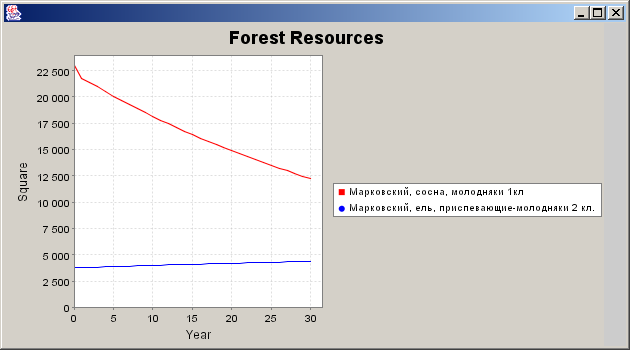
\includegraphics[width=449pt, height=249pt, keepaspectratio=true]{asyaDisser9_3-fig010.png}
%%\caption{This should be the caption for \texttt{asyaDisser9\_3-fig010.png}.}
%%\end{figure}

\begin{center}
Рис. 3.13. Результат работы скрипта - графики
\end{center}

Созданное приложение проводит расчеты по модели 
ДУД, с высоким уровнем рубок ухода и главного 
пользования и низким уровнем пожаров. Из полученных 
данных выделяются и добавляются к графику временной 
ряд значений площадей молодняков 1 кл. сосновых 
лесов Марковского лесхоза и ряд, который представляет 
собой разницу площадей приспевающих и молодняков 
2 класса ели Марковского лесхоза. Полученный 
график (объект-изображение) помещается на созданную 
форму и отображается пользователю.

Данный механизм позволяет управлять не только 
выводом графиков, но и такими возможностями 
информационной системы как расчеты по моделям, 
построение цифровых карт в ГИС.

Для того, чтобы вывести с помощью скрипта результаты 
расчетов на карту, у нему надо добавить строку:

js.makeMap(10, \texttt{"}сосна\texttt{"}, \texttt{"}спелые и перестойные\texttt{"}); 
 // карта для спелых и перестойных сосен десятого 
года интервала моделирования.

%%\begin{figure}[htbp]
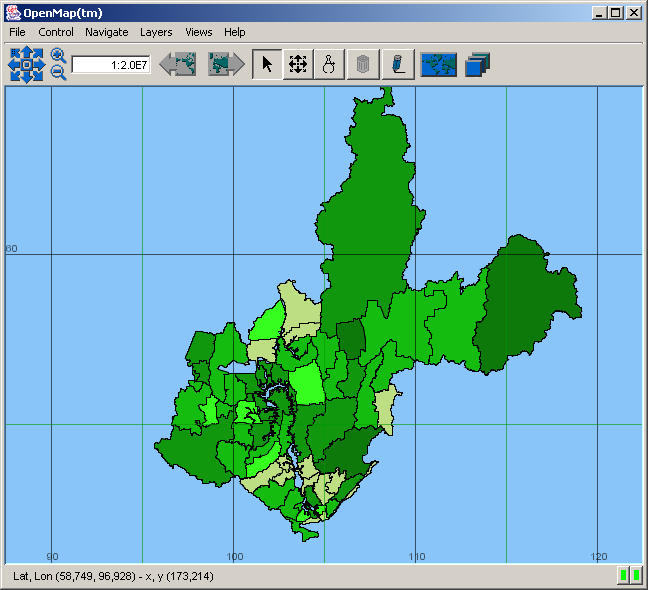
\includegraphics[width=452pt, height=412pt, keepaspectratio=true]{asyaDisser9_3-fig011.png}
%%\caption{This should be the caption for \texttt{asyaDisser9\_3-fig011.png}.}
%%\end{figure}

\begin{center}
Рис. 3.14. Результат работы скрипта - карта
\end{center}

Полученное приложение будет отображать карту 
площадей спелых и перестойных сосен десятого 
года интервала моделирования по лесхозам Иркутской 
области. Причем, чем темнее цвет окраски лесхоза 
на карте, тем больше в нем площадей указанной 
породы и класса возраста.

Возможность программирования скрипта является 
удобным инструментом для разработчиков. Например, 
с помощью скрипта можно создавать собственный 
интерфейс, импортировать исходные данные из 
форматов, неподдерживаемых информационной 
системой, анализировать результатные данные 
и т.д. Таким образом, модуль программирования 
javascript позволяет на основе Java-библиотеки jsCalc 
разработчикам создавать собственные варианты 
программного обеспечения для моделирования 
лесных ресурсов.\label{HToc199746738}

\textbf{3.4.2. Подсистема генерации карт и картографических 
анимаций}

Отображение картографических данных производится 
с помощью библиотеки OpenMap 4.6.3. OpenMap - это Java библиотека, 
позволяющая строить приложения и апплеты, оперирующие 
географической информацией. Она отображает 
картографические данные и осуществляет обработку 
запросов пользователей на манипулирование 
этими данными (масштабирование, перемещение, 
добавление слоев, сохранение и т.д.). Библиотека 
позволяет использовать данные форматов ESRI 
(шейп-файлы), а также данные из текстовых файлов 
CSV (comma-separated values) и некоторых других.

Для создания картографических произведений 
предназначен модуль информационной системы, 
который называется SimpleMap. \label{OLEHLINK18}\label{OLEHLINK19}В 
библиотеке OpenMap параметры создаваемой карты 
(пункты меню, слои, масштаб и т.д.) задаются в 
файле настроек openmap.properties. Данный файл представляет 
собой текстовый файл, в котором перечисляется 
последовательность параметров библиотеки 
OpenMap и присвоенных им значений, что позволяет 
управлять внешним видом отображаемой информации 
без изменения программных кодов библиотеки.\label{OLEHLINK4}\label{OLEHLINK5}

В информационной системе предусмотрена возможность 
создания карты по результатам прогнозных расчетов, 
на которой каждая расчетная единица (например, 
лесхоз) обозначается некоторым цветом в зависимости 
от численного значения расчетной характеристики. 
Поэтому, после проведения расчетов по всем 
лесхозам области пользователь имеет возможность 
посмотреть, как распределяются лесные ресурсы 
по территории области. Для создания картографического 
произведения необходимо выбрать характеристику 
лесных ресурсов - переменную модели или некоторое 
математическое выражение над переменными, 
которая должна быть отображена. Например, переменной 
обозначается доля площади лесов хвойной породы 
спелого класса возраста. После этого данные 
расчетной базы данных разделяются на группы 
в зависимости от установленных диапазонов 
значений, и различным объектам карты присваиваются 
соответствующие значения раскраски. Для раскраски 
берутся относительные значения характеристики, 
например, отношение площади молодняков сосны 
к общей площади лесхоза. Более темные цвета 
соответствуют большему значению характеристики, 
более светлые - меньшему.

Для отображения результатов в виде картографического 
произведения данные из баз данных расчета передаются 
в ГИС-подсистему, которая производит их отображение 
с привязкой к топооснове и сетке границ выделов. 
В качестве топоосновы в настоящее время используются 
карта лесхозов Иркутской области и квартальной 
сети Усть-Илимского района. Система позволяет 
строить картографические произведения для 
любого момента времени расчета модели, при 
этом существует возможность экспортировать 
изображения в файл (формата JPEG) и затем строить 
анимационные изображения. 

Кроме анимационных изображений на основе JPEG-файлов 
система позволяет для каждой стадии расчета 
динамики лесов формировать новое изображение 
как новый слой тематической карты. Динамика 
объекта исследования представляется серией 
картографических слоев, помеченных соответствующим 
моментом времени. Эти слои при последовательном 
подключении формируют картографическую анимацию, 
отображающую изменение во времени и в пространстве 
различных характеристик лесов.\label{HToc128995783}\label{HToc199746739}

\textbf{3.4.3. Подсистема запросов к структуре моделей 
и расчетным данным }

При большом разнообразии исходных данных, математических 
моделей и их параметров очень важно так организовать 
систему, чтобы она могла гибко настраиваться 
на проведение конкретных расчетов и специфику 
исходных данных. Поэтому в состав информационной 
системы включена интеллектная подсистема, 
реализованная при помощи языка логического 
программирования Prolog. Она содержит базу знаний 
(п. 3.3.5) \label{OLEHLINK36}\label{OLEHLINK37}о структурной и параметрической 
идентификации моделей динамики лесных ресурсов. 
Кроме того, интеллектная подсистема реализует 
вопросно-ответную подсистему, при помощи которой 
можно делать запросы к параметрам модели, результатам 
компьютерного моделирования.

В начале разработки данного модуля произведен 
анализ различных java-реализаций Пролога, например, 
таких как Jess, tuProlog, K-Prolog, Prolog Cafe и т.д. Из них для 
работы был выбран tuProlog [22] как проект, который 
активно развивается в настоящее время, позволяет 
использовать в java-программе правила вывода 
Пролога, обладает достаточно подробной документацией 
и является свободно распространяемой библиотекой 
с открытым исходным кодом.

Таким образом, для того, чтобы можно было использовать 
возможности Пролога в информационной системе, 
используется java-библиотека \label{OLEHLINK2}tuProlog 2.1. 
Данная библиотека является основанной на языке 
Java реализацией Пролога. При использовании tuProlog 
любые сущности Java (объекты, классы, пакеты) могут 
быть представлены в виде термов Пролога и быть 
использованы в Прологе. Также библиотека tuProlog 
может быть вызвана из Java-программы и использована 
в качестве java-объекта. tuProlog легко может быть 
внедрен в java-апплет для построения интеллектных 
Web-апплетов.

Для использования Пролога в программе создается 
экземпляр класса Prolog, который позволяет загружать 
код Пролога, загружать/выгружать библиотеки, 
достигать цели пролог-программы. Класс Theory 
представляет так называемую теорию Пролога, 
которая формализует предметную область. Теория 
является текстом, состоящим из последовательностей 
правил, каждое из которых завершается точкой 
и пробелом. Экземпляры этого класса создаются 
либо из текстового представления (строки типа 
String), либо из любого возможного входного потока 
(например, файла).

Класс SolveInfo позволяет проверить успешность 
запроса, получить доступ к его результату. Экземпляры 
этого класса возвращаются при обращении к методу 
solve класса Prolog. Если существуют термы, удовлетворяющие 
условиям запроса, то можно их все вывести пользователю. 
Таким образом, с помощью библиотеки tuProlog можно 
использовать правила вывода Пролога в информационной 
системе. 

Когда пользователь начинает расчет прогноза 
состояния ЛР с помощью информационной системы, 
то ему необходимо указать некоторые начальные 
данные о природном объекте (например, тип геосистемы) 
и задаче прогнозирования (например, длительность). 
Например, начальные данные для модели \texttt{"}Динамики 
управления древостоем\texttt{"} (ДУД) имеют следующий 
вид:

\textit{models(dud, problem(model\_dinam), rang(land), type(les), progn(desytilet)),}

т.е., начальные данные - это утверждение, представленное 
в виде факта языка Пролог. В приведенном примере 
утверждение означает, что для модели ДУД  характерно 
моделирование динамики объекта ранга ландшафта, 
 тип ландшафта - лес, временной интервал моделирования 
- десятилетия.

После того, как с помощью БЗ и механизма логического 
вывода будет найдена модель, подходящая для 
конкретной задачи прогнозирования, начнется 
построение выбранной модели. Например, для 
модели ДУД состояние объекта моделирования 
в начальный момент времени t0  получаем, используя 
правило
\textit{fs0(model(dud), Lesh, S, Snep, Nas) :- s0(Lesh, t0, S, Snep, Nas).}

Результатом работы правила будут общая площадь 
\textit{S}, не покрытая площадь \textit{Snep} и численность 
населения \textit{Nas} для лесхоза \textit{Lesh}.

Исходные данные о площадях, занятых породой 
определенного класса возраста получаются с 
помощью правил вида

\begin{center}
\textit{square(Lesh, Prd, vozrast(\texttt{"}молодняки 1кл \texttt{"}), 
t0, S) :-}

\textit{:- sq(Lesh, Prd, \_, S,\_, \_, \_, \_).}
\end{center}

Структура типа \textit{sq(Lesh, Prd, S, Sm1, Sm2, Ssr, Spr, Ssp4) 
}содержит данные о площадях лесхоза \textit{Lesh} 
породы \textit{Prd:} общей \textit{S}, молодняков 1 кл. 
\textit{Sm1} и 2 кл \textit{Sm2}, средневозрастных \textit{Ssr}, 
приспевающих \textit{Spr}, спелых и перестойных \textit{Ssp}.

После того, как из БЗ получены все исходные 
данные, начинается построение последовательности 
смены участками леса своих возрастных классов 
по модели ДУД с помощью следующего правила:

\textit{perehod(model(dud), Prd, Kl, Kl2, In) :- smena(Kl2, Kl), intens(Prd, In).}

«В модели ДУД переход леса породы \textit{Prd} из 
класса \textit{Kl} в класс \textit{Kl2} с интенсивностью\textit{ 
In }осуществляется, если \textit{Kl2 }сменяет \textit{Kl} 
и интенсивность для породы \textit{Prd} равна \textit{In}».

Смена классов возраста представлена термами 
вида \textit{smena(\texttt{"}молодняки 2кл\texttt{"}, \texttt{"}молодняки 
1кл\texttt{"}).}

Используя это правило, строится матрица коэффициентов 
перехода площадей леса из одного состояния 
в другое, проводятся численные расчеты. Также 
при этом может быть учтено проведение в лесах 
рубок главного пользования. Правило проведения 
рубок выглядит следующим образом:

\begin{center}
\textit{rubkaGP(model(dud), porod(K), vozrast(V), Vr) :-}

\textit{:-  porodRub(K), rubkaGP\_type(V), rubGP(K, Vr).}

\textit{rubkaGP\_type(\texttt{"}спелые и перестойные\texttt{"}).}
\end{center}

«В модели ДУД рубки главного пользования по 
породе \textit{K} возраста \textit{V} объемом \textit{Vr} 
проводятся, если порода \textit{K} может вырубаться, 
ее возраст \textit{V} подлежит вырубке и объем ее 
рубки составляет\textit{ Vr}».

При этом породами, которые могут вырубаться 
\textit{porodRub() }являются все  сосна, лиственница, 
пихта, ель, береза и осина (кроме кедра). Также 
для рубок главного пользования предназначены 
только деревья спелого и перестойного класса 
возраста \textit{rubkaGP\_type()}.

Далее по построенной структуре модели и полученным 
исходным данным информационной системой проводятся 
 прогнозные расчеты. 

Алгоритм загрузки кода Пролога и обработки 
его результатов выглядит следующим образом: 

Prolog engine (unknown char) new Prolog();     \textit{// создаем экземпляр 
класса Prolog}

engine.setTheory(new Theory(new FileInputStream(\texttt{"}model.pl\texttt{"}))); 
\textit{//   загрузка файла базы знаний}

SolveInfo info(unknown char)engine.solve(query);     \textit{// запрос к 
базе}

if (info.isSuccess())\{        \textit{//если есть решение, то... 
 }

String res (unknown char) info.getSolution(). toString();    \textit{// получаем 
решение  }

if (engine.hasOpenAlternatives())    \textit{//если есть еще решения 
   }

info (unknown char) engine.solveNext();      \textit{// обрабатываем 
следующее}

else break;    \textit{// иначе заканчиваем}

База знаний содержит правила, позволяющие производить 
идентификацию математической модели. Это дает 
возможность описывать сложные закономерности 
динамики природных объектов. Также для гибкой 
подстройки модели к условиям региона не требуется 
изменять код информационной системы расчета 
прогноза, а необходимо лишь внести требуемые 
данные в базу знаний или дополнить ее новыми 
правилами. \pagebreak{}\label{HToc199746740}

\section*{\textbf{Глава 4. Приложения информационной 
системы\label{HToc199746741}}}

\subsubsection*{\textbf{4.1. Моделирование динамики лесов 
Иркутской области по модели ДУД}}

Рассмотрим результаты расчетов при моделировании 
динамики лесов по лесхозам Иркутской области 
по модели ДУД, сценарий учитывал проведение 
полного цикла рубок ухода и главного пользования, 
отсутствие пожаров и лесопосадок. В качестве 
исходных данных были взяты данные распределения 
площадей лесов по породам и группам возраста 
по состоянию на 1 января 2004 г. Расчет производился 
по всем лесхозам, на 30 лет.

Интенсивность рубок для каждой породы и класса 
возраста задана правилами БЗ согласно [61, 70]. 
Во время рубок главного пользования вырубаются 
леса только спелого и перестойного класса возраста, 
всех пород, кроме кедра. Интенсивность рубок 
главного пользования задана для сосны и лиственницы 
60\%, для пихты и ели 40\%, для березы и осины 100\%. 
Интенсивности рубок ухода по породам и классам 
возраста приведены в таблице 2.

\begin{flushright}
Таблица 2. Интенсивности рубок ухода

\begin{tabular}{|>{\raggedright}p{104pt}|>{\raggedright}p{155pt}|>{\raggedright}p{115pt}|}
\hline
Порода & Класс возраста & Интенсивность, \%\tabularnewline
\hline
кедр & молодняки 1кл. & 30\tabularnewline
\hline
кедр & молодняки 2кл. & 20\tabularnewline
\hline
кедр & средневозрастные & 15\tabularnewline
\hline
кедр & спелые и перестойные & 100\tabularnewline
\hline
сосна & молодняки 2кл. & 20\tabularnewline
\hline
сосна & средневозрастные & 20\tabularnewline
\hline
сосна & приспевающие & 25\tabularnewline
\hline
лиственница & молодняки 2кл. & 30\tabularnewline
\hline
лиственница & средневозрастные & 20\tabularnewline
\hline
лиственница & приспевающие & 25\tabularnewline
\hline
ель & молодняки 2кл. & 30\tabularnewline
\hline
ель & средневозрастные & 20\tabularnewline
\hline
ель & приспевающие & 25\tabularnewline
\hline
пихта & молодняки 2кл. & 30\tabularnewline
\hline
пихта & средневозрастные & 20\tabularnewline
\hline
пихта & приспевающие & 15\tabularnewline
\hline
береза & средневозрастные & 20\tabularnewline
\hline
береза & приспевающие & 20\tabularnewline
\hline
осина & средневозрастные & 30\tabularnewline
\hline
осина & приспевающие & 20\tabularnewline
\hline
\end{tabular}
\end{flushright}

Динамика лесных ресурсов при заданных параметрах 
может быть представлена в виде следующего графа 
(рис. 4.1), на котором кроме естественной динамики 
также отражено проведение рубок ухода и главного 
пользования:

\begin{center}
%%\begin{figure}[htbp]
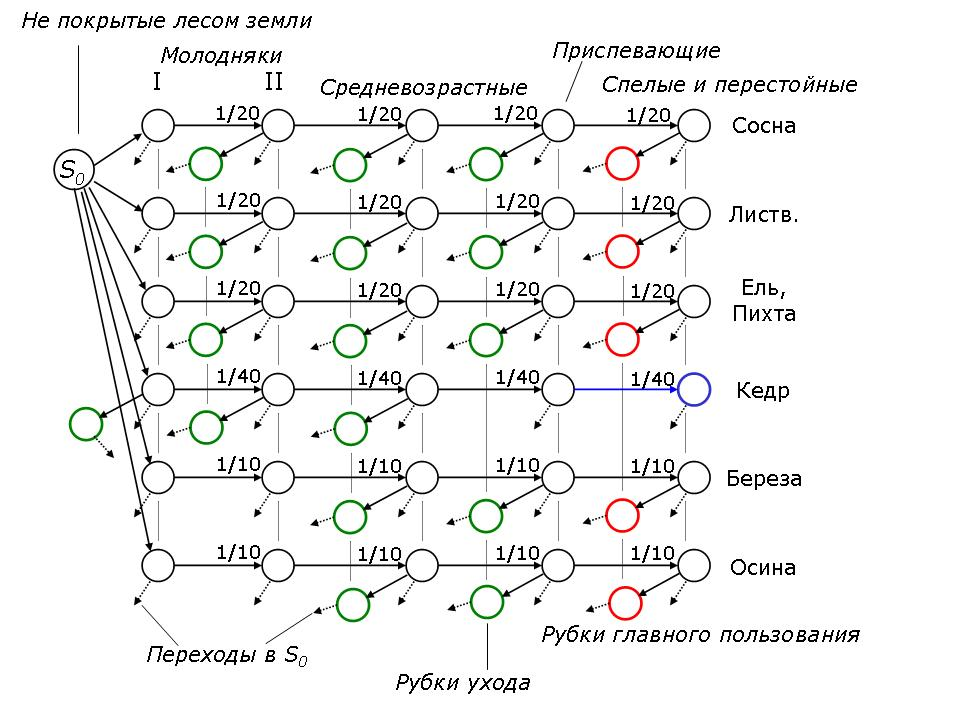
\includegraphics[width=490pt, height=346pt, keepaspectratio=true]{asyaDisser9_3-fig012.png}
%%\caption{This should be the caption for \texttt{asyaDisser9\_3-fig012.png}.}
%%\end{figure}

Рис. 4.1. Полученный граф динамики ЛР

%%\begin{figure}[htbp]
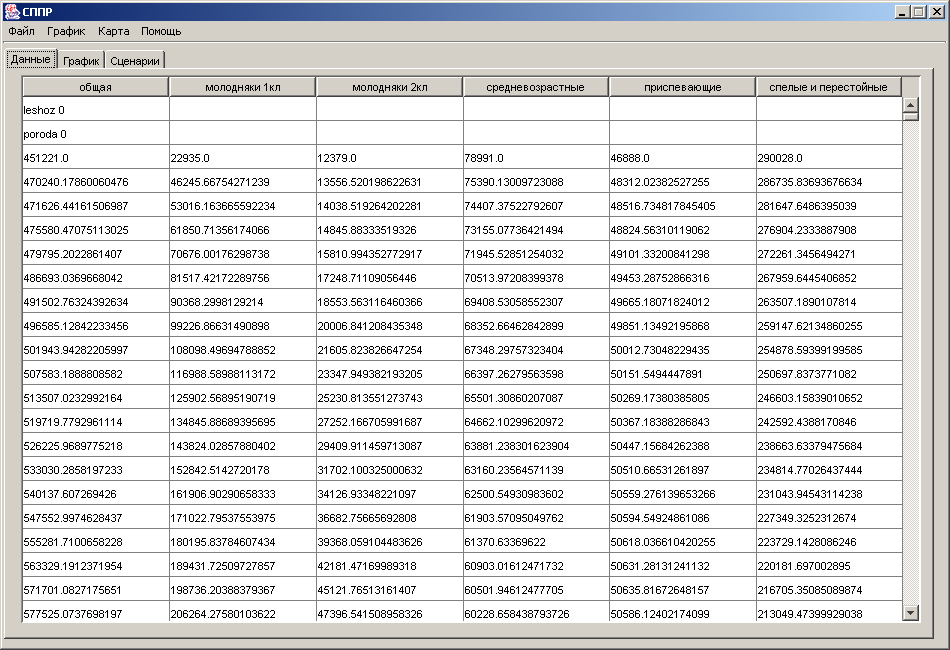
\includegraphics[width=449pt, height=312pt, keepaspectratio=true]{asyaDisser9_3-fig013.png}
%%\caption{This should be the caption for \texttt{asyaDisser9\_3-fig013.png}.}
%%\end{figure}

Рис. 4.2. Результаты расчетов по модели ДУД 

%%\begin{figure}[htbp]
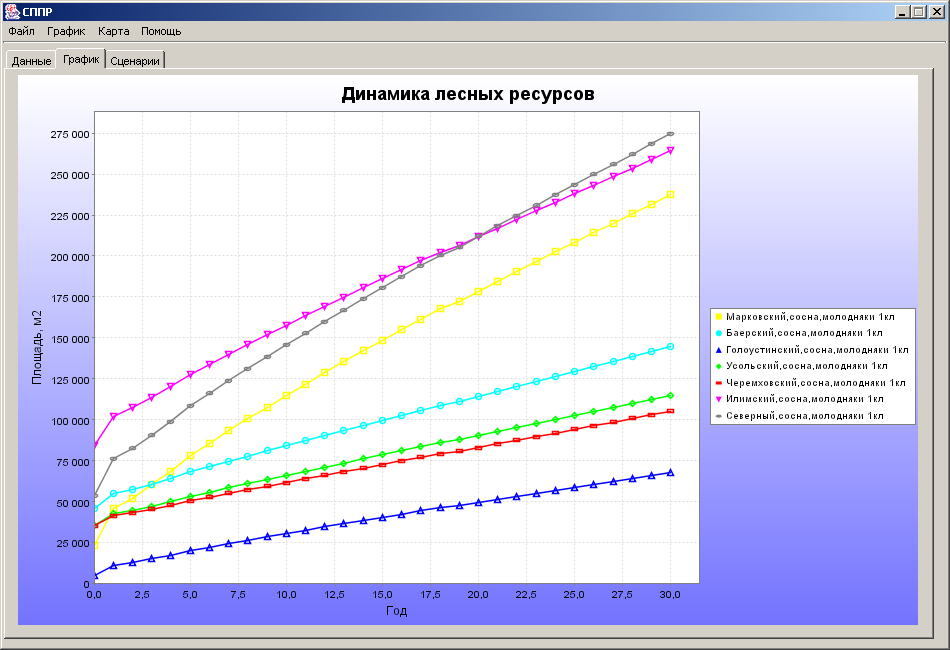
\includegraphics[width=449pt, height=307pt, keepaspectratio=true]{asyaDisser9_3-fig014.png}
%%\caption{This should be the caption for \texttt{asyaDisser9\_3-fig014.png}.}
%%\end{figure}

Рис. 4.3. График динамики состояния лесных ресурсов 
по молоднякам 1 кл.

%%\begin{figure}[htbp]
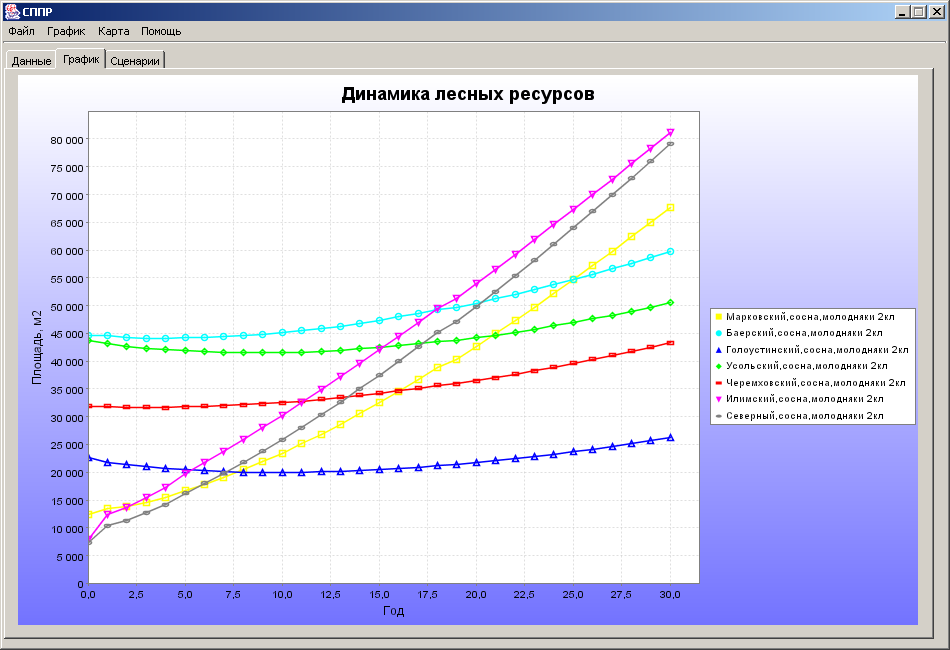
\includegraphics[width=449pt, height=307pt, keepaspectratio=true]{asyaDisser9_3-fig015.png}
%%\caption{This should be the caption for \texttt{asyaDisser9\_3-fig015.png}.}
%%\end{figure}

Рис. 4.4. График динамики состояния лесных ресурсов 
по молоднякам 2 кл.

%%\begin{figure}[htbp]
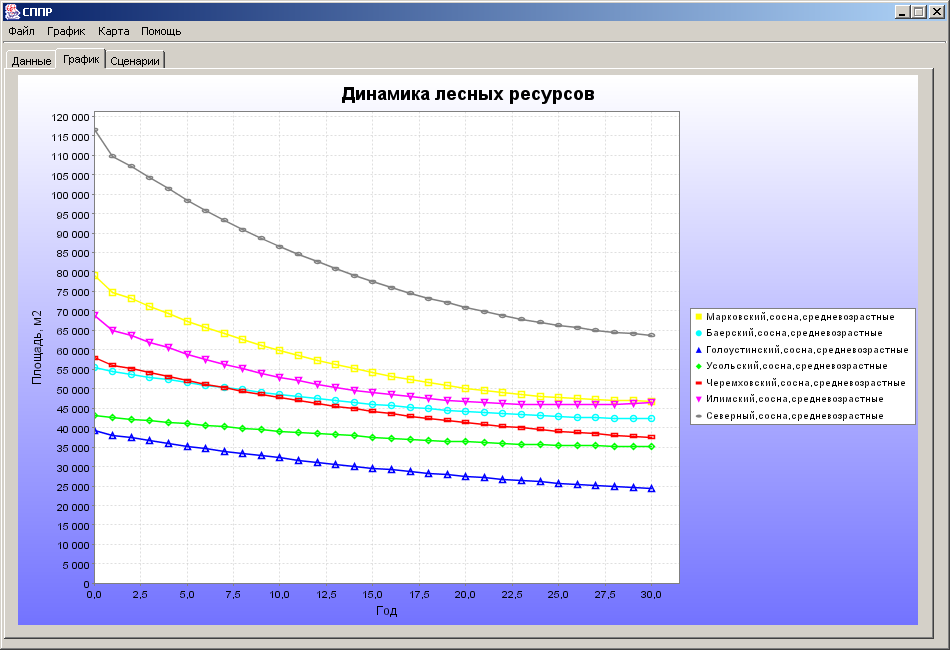
\includegraphics[width=449pt, height=307pt, keepaspectratio=true]{asyaDisser9_3-fig016.png}
%%\caption{This should be the caption for \texttt{asyaDisser9\_3-fig016.png}.}
%%\end{figure}

Рис. 4.5. График динамики состояния лесных ресурсов 
по средневозрастным

%%\begin{figure}[htbp]
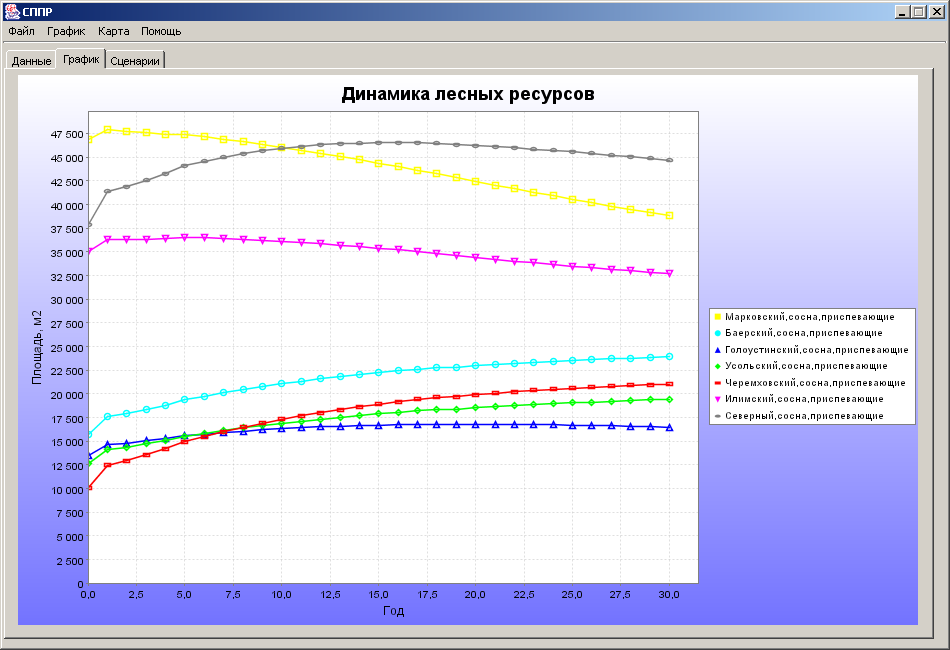
\includegraphics[width=449pt, height=307pt, keepaspectratio=true]{asyaDisser9_3-fig017.png}
%%\caption{This should be the caption for \texttt{asyaDisser9\_3-fig017.png}.}
%%\end{figure}

Рис. 4.6. График динамики состояния лесных ресурсов 
по приспевающим

%%\begin{figure}[htbp]
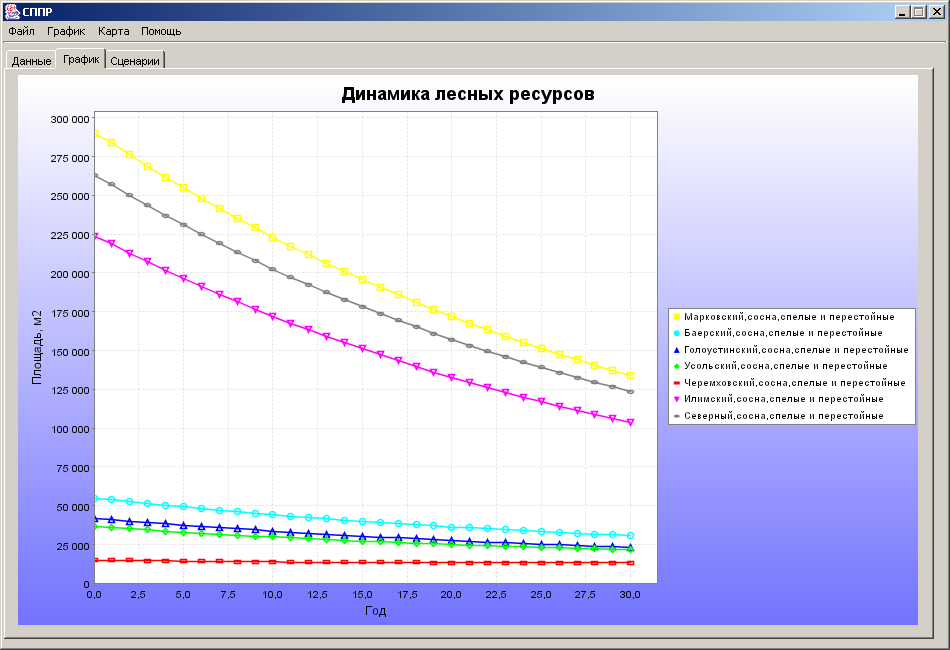
\includegraphics[width=449pt, height=307pt, keepaspectratio=true]{asyaDisser9_3-fig018.png}
%%\caption{This should be the caption for \texttt{asyaDisser9\_3-fig018.png}.}
%%\end{figure}

Рис. 4.7. График динамики состояния лесных ресурсов 
по спелым и перестойным
\end{center}

На рис. 4.3-4.7 приведены графики динамики состояния 
сосновых лесов всех классов возраста по нескольким 
выбранным лесхозам (Марковскому, Баерскому, 
Голоустинскому, Усольскому, Черемховскому, 
Илимскому и Северному). Для молодняков 1 класса 
(рис. 4.3) отмечается увеличение площадей по всем 
выбранным лесхозам, для молодняков 2 класса 
(рис. 4.4) также увеличиваются площади, но в некоторых 
лесхозах в первой половине интервала моделирования 
наблюдается небольшое их снижение. По средневозрастным 
(рис. 4.5) и спелым и перестойным (рис. 4.7) площади 
лесов во всех лесхозах уменьшаются. Причем 
в лесхозах с изначально большими площадями 
спелых и перестойных (Марковский, Северный, 
Илимский) наблюдается и более быстрое их уменьшение, 
почти в два раза (рис. 4.7.). По приспевающим (рис. 
4.6) в начале по всем лесхозам происходит увеличение 
площадей, к концу интервала моделирования в 
некоторых отмечается уменьшение площадей лесов.

Результаты расчетов по одному из классов возраста 
могут быть отображены на карте, для создания 
которой пользователю необходимо задать такие 
параметры как год из интервала моделирования, 
порода и класс возраста леса. Состояние сосновых 
лесов спелого и перестойного класса возраста 
на начало периода моделирования, через 10, 20 
и 30 лет приведено на рис. 4.8-4.11.

На каждом этапе моделирования становится заметным 
уменьшение площадей сосновых лесов спелого 
и перестойного класса возраста во всех лесхозах 
(рис. 4.8-4.11). Это обусловлено проведением полного 
цикла рубок (ухода и главного пользования) при 
отсутствии лесопосадок.

\begin{center}
%%\begin{figure}[htbp]
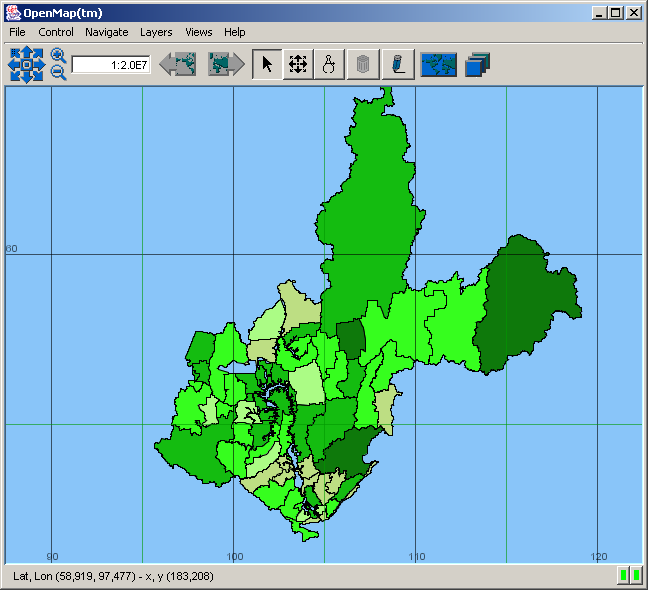
\includegraphics[width=452pt, height=407pt, keepaspectratio=true]{asyaDisser9_3-fig019.png}
%%\caption{This should be the caption for \texttt{asyaDisser9\_3-fig019.png}.}
%%\end{figure}

Рис. 4.8. Состояние лесов на начало периода моделирования

%%\begin{figure}[htbp]
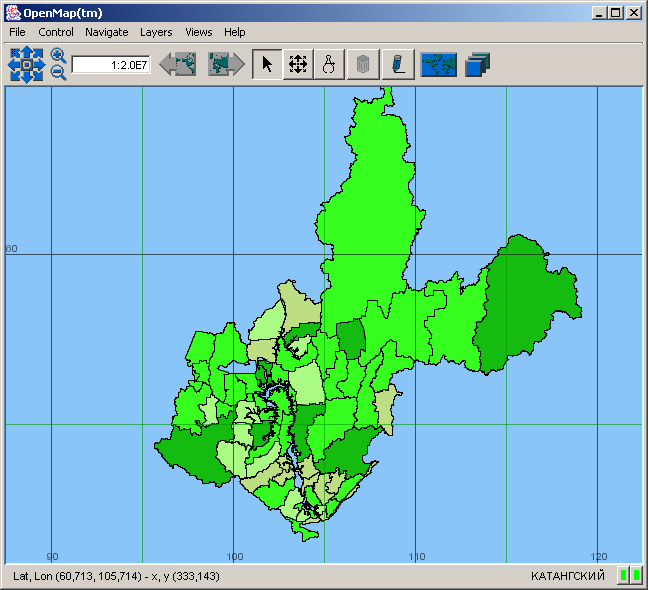
\includegraphics[width=452pt, height=407pt, keepaspectratio=true]{asyaDisser9_3-fig020.png}
%%\caption{This should be the caption for \texttt{asyaDisser9\_3-fig020.png}.}
%%\end{figure}

Рис. 4.9. Состояние  лесов через 10 лет

%%\begin{figure}[htbp]
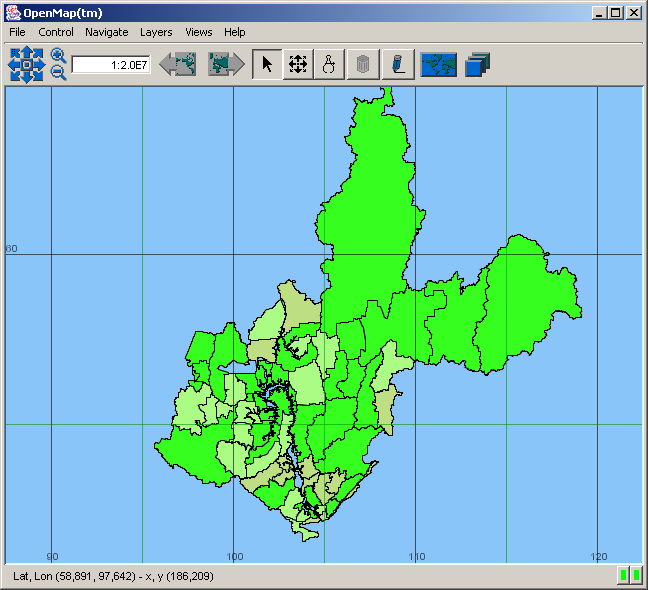
\includegraphics[width=452pt, height=407pt, keepaspectratio=true]{asyaDisser9_3-fig021.png}
%%\caption{This should be the caption for \texttt{asyaDisser9\_3-fig021.png}.}
%%\end{figure}

Рис. 4.10. Состояние  лесов через 20 лет

%%\begin{figure}[htbp]
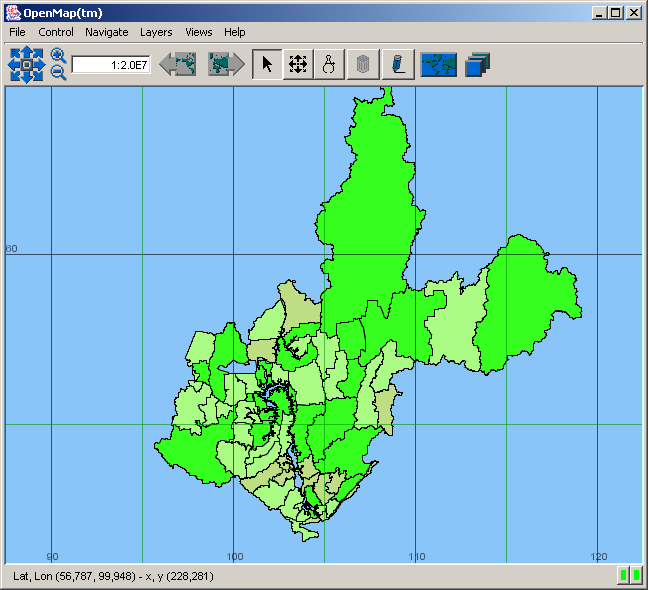
\includegraphics[width=452pt, height=407pt, keepaspectratio=true]{asyaDisser9_3-fig022.png}
%%\caption{This should be the caption for \texttt{asyaDisser9\_3-fig022.png}.}
%%\end{figure}

Рис. 4.11. Состояние  лесов через 30 лет
\end{center}

При таком сценарии использования ЛР (истощительные 
рубки) максимальный объем рубок по всей Иркутской 
области составит 202.6 млн. м3/год. При проведении 
рубок в половине объема и проведении лесовосстановительных 
мероприятий объем рубок по расчетам составит 
78.4 млн. м3/год. Расчетная лесосека для Иркутской 
области по данным на 2007 г. составляет 52.7 млн. 
м3/год, т.е. по расчетам возможно увеличение 
объемов заготовки леса в рамках неистощительного 
лесопользования (табл. 3).

\begin{flushright}
Таблица 3. Сравнение объемов рубок

\begin{tabular}{|>{\raggedright}p{151pt}|>{\raggedright}p{94pt}|>{\raggedright}p{58pt}|>{\raggedright}p{101pt}|}
\hline
~ & Площадь рубок, га & Запас на 1 га, м3 & Объем 
рубок,  млн. м3/год\tabularnewline
\hline
Сценарий 1 (истощительные рубки) & 1 164 376.07 & 232 & 202.6\tabularnewline
\hline
Сценарий 2 (рубки+посадки) & 450 727.83 & 232 & 78.4\tabularnewline
\hline
Расчетная лесосека на 2007 г.~ & ~ &  & 52.7\tabularnewline
\hline
\end{tabular}
\end{flushright}

В табл. 4 приведены результаты выделения множества 
парето-оптимальных решений и значения параметров 
по 10 сценариям для всех лесхозов Иркутской 
области. В столбце «Парето» значение 1 соответствует 
тому, что данный критерий вошел в это множество, 
значение 0 - не вошел. 

\begin{flushright}
Таблица 4. Результаты выделения парето-оптимальных 
решений из 10 сценариев моделирования

\begin{tabular}{|>{\raggedright}p{12pt}|>{\raggedright}p{50pt}|>{\raggedright}p{51pt}|>{\raggedright}p{73pt}|>{\raggedright}p{65pt}|>{\raggedright}p{23pt}|>{\raggedright}p{94pt}|}
\hline
º & V\textsuperscript{j}\textsubscript{b}(t\textsubscript{i}) & S\textsuperscript{j}\textsubscript{g}(t\textsubscript{i}) & S\textsuperscript{j}\textsubscript{p}+S\textsuperscript{j}\textsubscript{s} & V\textsuperscript{j}\textsubscript{р}(t\textsubscript{i}) & Парето & Параметры\tabularnewline
\hline
1.  & 280236.61 & 350489.43 & 527734841.80 & 24207380.32 & 1 & уход 88, рубки 
100, пожары 79, посадки 94\tabularnewline
\hline
2.  & 282801.24 & 350195.47 & 475614762.22 & 15313280.93 & 0 & уход 0, рубки 
100, пожары 50, посадки 0\tabularnewline
\hline
3.  & 284838.00 & 349346.04 & 531294730.52 & 17306464.04 & 1 & уход 21, рубки 
90, пожары 44, посадки 55\tabularnewline
\hline
4.  & 257937.40 & 357486.35 & 574898921.96 & 11384313.66 & 0 & уход 9, рубки 
55, пожары 97, посадки 10\tabularnewline
\hline
5.  & 281357.42 & 348606.29 & 666213019.11 & 14099211.53 & 1 & уход 45, рубки 
45, пожары 84, посадки 78\tabularnewline
\hline
6.  & 275729.63 & 349545.51 & 732608072.31 & 4973020.68 & 0 & уход 47, рубки 
5, пожары 91, посадки 6\tabularnewline
\hline
7.  & 287345.63 & 347425.80 & 663062677.09 & 12488359.39 & 1 & уход 8, рубки 
53, пожары 50, посадки 92\tabularnewline
\hline
8.  & 248732.28 & 362002.10 & 584442958.36 & 10785954.30 & 0 & уход 11, рубки 
50, пожары 98, посадки 9\tabularnewline
\hline
9.  & 288192.75 & 347372.72 & 770641427.03 & 6275922.76 & 1 & уход 45, рубки 
9, пожары 6, посадки 50\tabularnewline
\hline
10.  & 285106.83 & 348836.46 & 584290631.75 & 10962106.35 & 0 & уход 6, рубки 
53, пожары 47, посадки 7\tabularnewline
\hline
\end{tabular}
\end{flushright}

Таким образом, из 10 сценариев было отсечено 
5. Оптимальными сценариями для управления лесными 
ресурсами по заданному набору критериев являются: 

1) проведение в полном объеме рубок главного 
пользования, рубок ухода и лесопосадок, с учетом 
текущего числа пожаров в лесах области; 

2) минимальный уровень рубок ухода, проведение 
рубок главного пользования в полном объеме, 
лесопосадок - в половине объема, уменьшение 
количества пожаров в 2 раза; 

3) проведение рубок главного пользования и рубок 
ухода в половине объема, полного уровня лесопосадок, 
при текущем числе пожаров; 

4) минимальный уровень рубок ухода, проведение 
рубок главного пользования в половине объема, 
лесопосадок - в полном объеме, уменьшение количества 
пожаров в 2 раза; 

5) увеличение лесопокрытых площадей и запасов 
древесины по всем группам возраста - минимальные 
рубки главного пользования, проведение рубок 
ухода в половине объема, лесопосадок - в полном 
объеме, минимум пожаров.

В рассмотренном примере объемы рубок ухода 
и главного пользования определялись в зависимости 
от породы и класса возраста и не зависели от 
текущего состояния ЛР на каждом этапе моделирования. 
Можно задать другую стратегию рубок - например, 
дополнить базу знаний информационной системы 
правилами уменьшения объема рубок при снижении 
лесной площади лесхоза ниже заданного уровня. 
Или промоделировать рубки при нарушении действующего 
законодательства [61, 70] - ведение рубок главного 
пользования во всех классах возраста, вырубка 
кедра. Таким образом, информационная система 
может быть подстроена под конкретную задачу 
пользователя.\label{HToc199746742}

\subsubsection*{\textbf{4.2. Моделирование динамики лесов 
Усть-Илимского района по модели «Лесные ресурсы»}}

Рассмотрим результаты расчетов при моделировании 
динамики лесов по модели «Лесные ресурсы», 
с учетом проведения рубок главного пользования: 
насаждения различного возраста вырубаются 
в кварталах с достаточным запасом древесины, 
расположенных на расстоянии \textit{L }(unknown char) 
90 км от вектора направления рубки. Направление 
вектора рубок в данном примере показано на 
рис. 4.12 красной стрелкой, соответственно рубки 
рассчитывались только для территории, примерно 
очерченной пунктирной окружностью. Вектор 
рубки задается парами координат начального 
(x\textsubscript{0}, y\textsubscript{0}) и конечного квартала 
(x\textsubscript{1}, y\textsubscript{1}). Координаты кварталов 
содержатся в исходных данных и представляют 
собой координаты центра квартала (п. 3.3.1). Расчеты 
велись для территории Усть-Илимского района 
на 100 лет, максимальный объем рубок был задан 
в 3000 тыс. м\textsuperscript{3}/год, 1325 тыс. м\textsuperscript{3}/год 
(расчетная лесосека для выбранного района по 
состоянию на 1 января 2006 года) и 700 тыс. м\textsuperscript{3}/год. 
Карты состояния лесов спелого и перестойного 
класса возраста в начальный момент моделирования, 
через 100 лет для каждого значения максимального 
объема рубки приведены на рисунках 4.12-4.15.

\begin{center}
%%\begin{figure}[htbp]
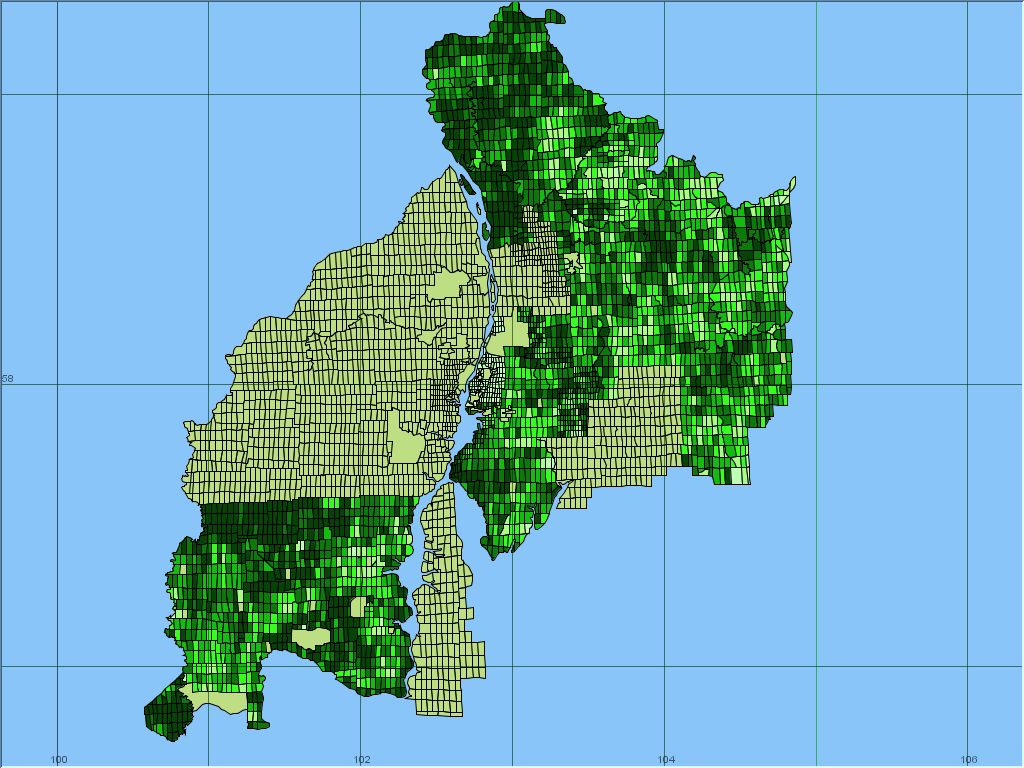
\includegraphics[width=607pt, height=461pt, keepaspectratio=true]{asyaDisser9_3-fig023.jpg}
%%\caption{This should be the caption for \texttt{asyaDisser9\_3-fig023.jpg}.}
%%\end{figure}

Рис. 4.12. Состояние лесов на начало периода моделирования
\end{center}

Если максимальный объем рубки равен \label{OLEHLINK34}\label{OLEHLINK35}3000 
тыс. м\textsuperscript{3}/год, то по расчетам запасов 
хватит только на 21 год (табл. 5), после чего объемы 
рубок начнут снижаться и к концу интервала 
моделирования уменьшаться почти в три раза 
(до 1183.45 тыс. м\textsuperscript{3}/год).

\begin{flushright}
Таблица 5. Значения критериев рубки

\begin{tabular}{|>{\raggedright}p{40pt}|>{\raggedright}p{92pt}|>{\raggedright}p{138pt}|>{\raggedright}p{138pt}|}
\hline
Год & Объем рубки & Iq & Iw\tabularnewline
\hline
1 & 3000.0 & 126 438.68 & 150.00\tabularnewline
\hline
10 & 3000.0 & 6 884 979.13 & 1 500.00\tabularnewline
\hline
21 & 3000.0 & 28 579 354.73 & 3 150.00\tabularnewline
\hline
22 & 2978.83 & 31 268 600.46 & 3 298.94\tabularnewline
\hline
40 & 2401.08 & 99 541 322.99 & 5 695.74\tabularnewline
\hline
50 & 2131.52 & 153 347 593.68 & 6 820.79\tabularnewline
\hline
60 & 1893.23 & 218 183 096.70 & 7 819.83\tabularnewline
\hline
70 & 1682.28 & 293 846 215.26 & 8 707.37\tabularnewline
\hline
80 & 1495.50 & 380 167 173.93 & 9 496.20\tabularnewline
\hline
90 & 1330.18 & 477 004 244.50 & 10 197.63\tabularnewline
\hline
100 & 1183.45 & 584 240 389.89 & 10 821.63\tabularnewline
\hline
\end{tabular}
\end{flushright}

\begin{center}
%%\begin{figure}[htbp]
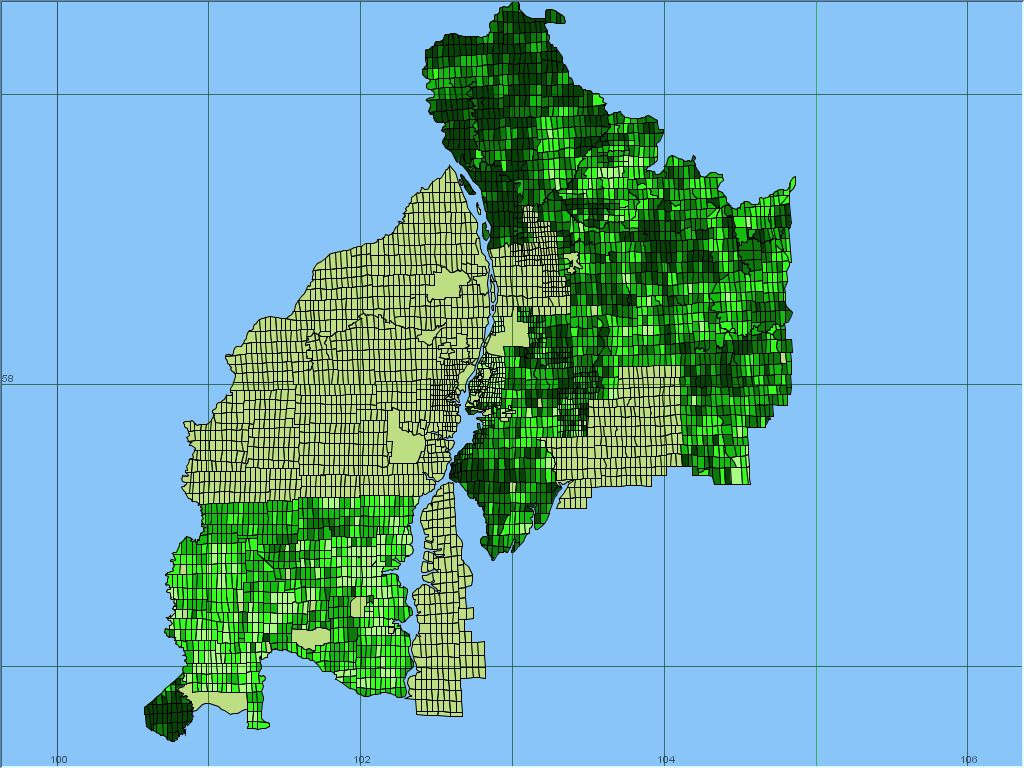
\includegraphics[width=622pt, height=467pt, keepaspectratio=true]{asyaDisser9_3-fig024.png}
%%\caption{This should be the caption for \texttt{asyaDisser9\_3-fig024.png}.}
%%\end{figure}

Рис. 4.13. Состояние лесов через 100 лет, объем рубки 
3000 тыс. м\textsuperscript{3}/год
\end{center}

Рубки в данном примере затрагивают только нижнюю 
левую часть территории, поэтому в этом районе 
наблюдается значительное уменьшение площадей 
лесов спелого и перестойного класса возраста. 
На остальной территории в отсутствии рубок 
наблюдается увеличение площадей лесов (рис. 
4.13). Из результатов расчетов следует, что объемы 
рубки в 3000 тыс. м\textsuperscript{3}/год являются истощительными 
для данной территории и приведут к существенному 
уменьшению площадей лесов.

В таблице 6 приведены численные значения критериев 
рубки при расчетах на 100 лет с максимальным 
объемом рубки, равным расчетной лесосеке для 
выбранной территории по состоянию на 1 января 
2006 года (1325 тыс. м\textsuperscript{3}/год). По результатам 
расчетов при таких параметрах рубки будут вестись 
с максимальной мощностью 48 лет, после чего их 
объемы начнут снижаться до 1007.83 тыс. м\textsuperscript{3}/год 
через 100 лет. Однако в данном примере не учитывались 
лесопосадки, поэтому проведение рубок такой 
мощности в течение длительного времени возможно 
только совместно с лесовосстановительными 
мероприятиями.

\begin{flushright}
Таблица 6. Значения критериев рубки

\begin{tabular}{|>{\raggedright}p{39pt}|>{\raggedright}p{98pt}|>{\raggedright}p{133pt}|>{\raggedright}p{133pt}|}
\hline
Год & Объем рубки & Iq & Iw\tabularnewline
\hline
1 & 1325.0 & 126 501.48 & 66.25\tabularnewline
\hline
20 & 1325.0 & 26 095 786.61 & 1 325.00\tabularnewline
\hline
40 & 1325.0 & 100 114 833.18 & 2 650.00\tabularnewline
\hline
48 & 1325.0 & 142 613 842.31 & 3 180.00\tabularnewline
\hline
49 & 1318.42 & 148 432 683.81 & 3 245.92\tabularnewline
\hline
60 & 1243.89 & 219 762 108.14 & 3 948.49\tabularnewline
\hline
80 & 1119.45 & 383 126 564.15 & 5 125.91\tabularnewline
\hline
100 & 1007.83 & 588 661 215.90 & 6 185.77\tabularnewline
\hline
\end{tabular}
\end{flushright}

На карте состояния лесов при максимальном объеме 
рубок, равном расчетной лесосеке (рис. 4.14) также 
отмечается уменьшение площадей лесов на выбранной 
для рубок территории.

\begin{center}
%%\begin{figure}[htbp]
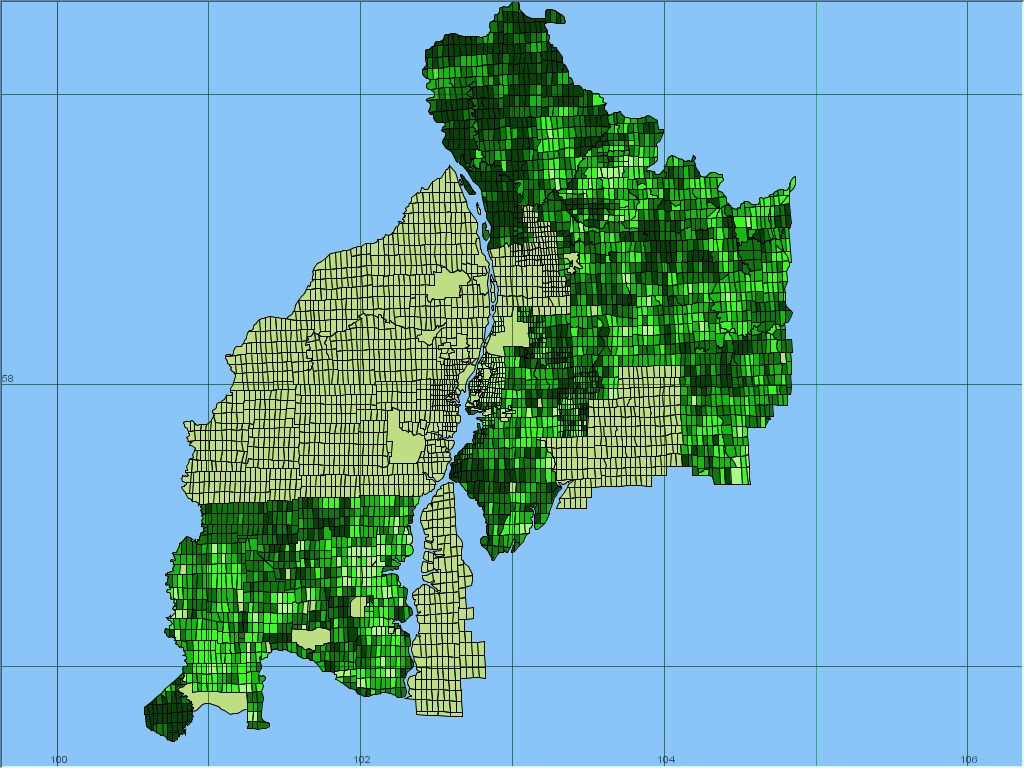
\includegraphics[width=622pt, height=467pt, keepaspectratio=true]{asyaDisser9_3-fig025.png}
%%\caption{This should be the caption for \texttt{asyaDisser9\_3-fig025.png}.}
%%\end{figure}

Рис. 4.14. Состояние лесов через 100 лет, рубки по 
расчетной лесосеке
\end{center}

В таблице 7 приведены численные значения критериев 
рубки при расчетах на 100 лет с максимальным 
объемом рубки 700 тыс. м\textsuperscript{3}/год. При такой 
стратегии использования лесных ресурсов запасов 
хватит почти на весь период моделирования: 
рубки будут вестись с максимальной мощностью 
93 года, после чего произойдет небольшое снижение 
их объема (до 686.57 тыс. м\textsuperscript{3}/год). 

\begin{flushright}
Таблица 7. Значения критериев рубки

\begin{tabular}{|>{\raggedright}p{38pt}|>{\raggedright}p{88pt}|>{\raggedright}p{132pt}|>{\raggedright}p{132pt}|}
\hline
Год & Объем рубки & Iq & Iw\tabularnewline
\hline
1 & 700.0 & 126 524.91 & 35.00\tabularnewline
\hline
20 & 700.0 & 26 128 406.35 & 700.00\tabularnewline
\hline
40 & 700.0 & 100 331 474.39 & 1 400.00\tabularnewline
\hline
60 & 700.0 & 220 393 260.27 & 2 100.00\tabularnewline
\hline
80 & 700.0 & 384 411 298.81 & 2 800.00\tabularnewline
\hline
93 & 700.0 & 513 814 414.76 & 3 255.00\tabularnewline
\hline
94 & 698.17 & 524 497 646.58 & 3 289.91\tabularnewline
\hline
100 & 686.57 & 590 760 723.18 & 3 497.33\tabularnewline
\hline
\end{tabular}
\end{flushright}

\begin{center}
%%\begin{figure}[htbp]
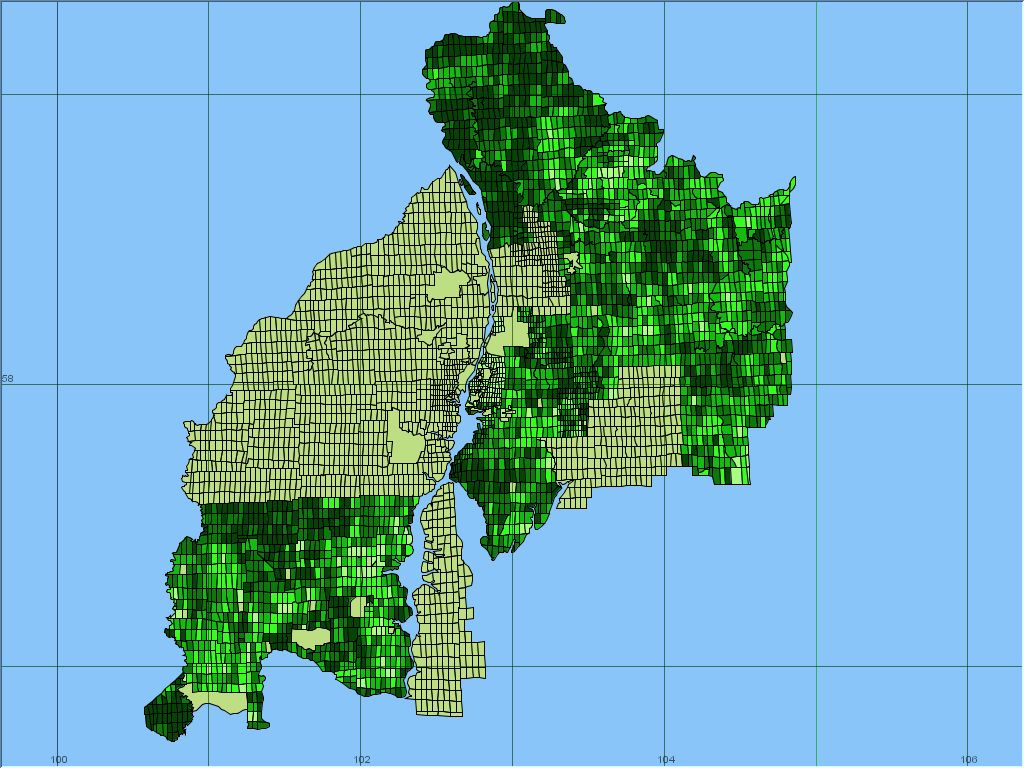
\includegraphics[width=622pt, height=467pt, keepaspectratio=true]{asyaDisser9_3-fig026.png}
%%\caption{This should be the caption for \texttt{asyaDisser9\_3-fig026.png}.}
%%\end{figure}

Рис. 4.15. Состояние лесов через 100 лет, объем рубки 
700 тыс. м\textsuperscript{3}/год
\end{center}

Таким образом, по результатам расчетов мощность 
рубок в 700 тыс. м3/год позволяет в течение 100 лет 
вести неистощительные заготовки леса даже 
при отсутствии лесопосадок.\pagebreak{}\label{HToc199746743}

\section*{\textbf{Заключение}}

Автором получены следующие основные теоретические 
и практические результаты:

1. Обоснована актуальность разработки информационной 
системы для ЛПР по рациональному использованию 
лесных ресурсов. Определены основные направления 
совершенствования реализованных ранее технологий 
исследования ЛР. 

2. Разработана методика конструирования информационной 
системы, основанная на комплексном подходе, 
включающем этапы идентификации математических 
моделей лесных ресурсов, расчета прогноза динамики, 
а также анализа критериев компьютерного моделирования.

3. Реализованы модели динамики ЛР «Динамика 
управления древостоем» и «Лесные ресурсы» 
и подсистема их параметрической идентификации.

4. Реализовано задание сценариев использования 
лесных ресурсов на основе различных комбинаций 
параметров модели, многокритериальная оптимизация 
рассчитанных сценариев по набору критериев.

5. Созданы инструментальные средства, которые 
позволяют конструировать специализированные 
информационные системы, направленные на поддержку 
решений задач ЛПР, связанных с анализом состояния 
и перспектив использования ЛР промышленного 
региона.

6. Информационная система и инструментальные 
средства апробированы в задачах прогнозирования 
ЛР Иркутской области, определены объемы рубок, 
позволяющие вести неистощительное использование 
ЛР.

В дальнейшем предполагается развивать ИС в 
направлении разработки программных технологий 
логико-математического моделирования динамики 
ЛР в рамках реализации заданной политики заготовки 
ЛР. Основу программных технологий будут формировать 
технологии формального описания правил принятия 
решения об уровне заготовки ЛР в заданные периоды 
времени, подсистемы параметрической идентификации 
математических моделей ЛР для заданного класса 
задач и масштаба исследуемой геосистемы, системы 
численных расчетов получаемых моделей и оценки 
значений критериев, подсистемы многокритериальной 
оптимизации получаемых решений, системы визуализации 
результатов анализа. \pagebreak{}\label{HToc128995786}\label{HToc199746744}

\section*{\textbf{Список использованной литературы}}

1. Botkin D.B., J.F. Janak, and JR. Wallis. Rationale, limitations and assumtions 
of a Northeastern Forest Growth Simulator. IBM J. Research Development 16, 1972. 
Pp. 101-116.

2. Botkin D.B., J.F. Janak, and JR. Wallis. Some ecological consequences of a computer 
model of forest growth. J. Ecol., 60, 1972. Pp. 849-872.

3. Bouil1е F. Making expert systems work in geographic information systems// Proc. 
13-th Int. Cartogr. conf.- Morelia.- 1988.- V.1.- P.109-122.

4. Bugmann H.K.M. A simplified forest model to study species composition along 
climate gradients. - Ecology, 1996, 77. - P. 2055-2074.

5. Connor D.J., Tunstall B.R. and Van den Driessche R. An analysis of photosynthetic 
response in a brigalow forest. Photosynthetica 5, 1971. Pp. 218-25.

6. Dixon, Gary E. comp. 2002. Essential FVS: A user's guide to the Forest Vegetation 
Simulator. Internal Rep. Fort Collins, CO: U. S. Department of Agriculture, Forest 
Service, Forest Management Service Center. 209p.

7. Estеs J.E., Sаilеr C.H., Tinnеy L.R. Applications of artificial intelligence 
techniques to remote sensing// The Profes. Geogr.-1986.- V.-38.-º2. P.133-141.

8. Fedra K., Winkelbauer L., Pantulu V.R. Eхpert Systems for Environmental Screening 
//RR-91-19 November 1991, International Institute for Applied Systems Analysis.- 
Laxenburg, Austria.- 170 p.

9. Fischlin, A., H. Bugmann, and D. Gyalistras. Sensitivity of a forest ecosystem 
model to climate parameterization schemes. Environmental Pollution 87, 1995. Pp. 
267-282.

10. Fishеr P.F., MаскаnеssW.A., Pеасеgood G.D., Wilкinson G.G. Artificial 
intelligence and expert systems in geodata processing// Progr. Phys. Gejgr.- 1988.- 
V.12.- º3.- Pp.371-388.

11. Forest Vegetation Simulator (FVS) [Электронный ресурс]/ USDA 
Forest Service, Forest Management Service Center. - Электрон. дан. - 
Режим доступа: http://www.fs.fed.us/fmsc/fvs/index.shtml, свободный.

12. Horn H. S. Markovian properties of forest succession // Ecology and Evolution 
of Communities. (Eds. M. Cody \& J. Diamond). - Cambridge, MA, Belknap, 1975. - 
Pp. 196-211. 

13. Horn H. S. Some causes of variety in patterns of forest succession // Forest 
Succession: Concepts and Applications. (Eds. D. C. West, H. H. Shugart, D. B. Botkin). 
-  N.Y., Springer-Verlag, 1991. - P. 24-35. 

14. LMS [Электронный ресурс]/ Landscape Management Project. - 
Электрон. дан. - University of Washington College of Forest Resources 
Silviculture Laboratory, Yale University School of Forestry and Environmental Studies, 
The Cradle of Forestry in America, and the USDA Forest Service, 2005-2007. - Режим 
доступа: http://lms.cfr.washington.edu/, свободный.

15. Mladenoff D.J., He H.S. Design and behavior of LANDIS, an object-oriented model 
of forest landscape disturbance and succession // Advances in Spatial Modeling 
of Forest Landscape Change: Approaches and Applications. (Eds. Mladenoff D.J., 
Baker W.L.). - Cambridge, UK, Cambridge University Press, 1999. - P. 125-162.

16. Mladenoff D.J., Host G.E., Boeder J., Crow T.R. LANDIS: a spatial model of 
forest landscape disturbance, succession, and management //. GIS and Environmental 
Modeling: Progress and Research Issues. (Eds. Goodchild M.F., Steyaert L.T., Parks 
B.O). - GIS World Inc., 1996. - P. 175-180.

17. Peden L. M., Williams J. S., \& Frayer W. E. A Markov model for stand projection. 
Forest Science, 19, 1973. Pp. 303-314.

18. Robinson V.B., Frаnк A.U. Expert systems for geographic information systems// 
Photogramm. Eng. and Remote Sens.- 1987.- V.53.- º10.- P.1435-1441.

19. Rudra A. Farm Size and Yield per Acre. Economic and Political Weekly 3(1), 
1968. - Pp. 23-34.

20. Shugart H. H. A Theory of Forest Dynamics. The Ecological Implications of Forest 
Succession Models. - N.Y., Springer, 1984. - p. 278.

21. Shugart H.H., Crow T.R., Hett J.M. Forest succession models: a rational and 
methodology for modeling forest succession over large regions - Forest Science, 
1973, vol. 19, º 3. - P. 203 -212.

22. tuProlog [Электронный ресурс]/ aliCE Research Group. - Электрон. 
дан. - DEIS:   Dipartimento di Elettronica, Informatica e Sistemistica, Alma 
Mater Studiorum Universita di Bologna, 1999-2006. - Режим доступа:http://www.alice.unibo.it:8080/tuProlog/, 
свободный.

23. Urban D.L., Harmon M.E., Halpern C.B. Potential response of Pacific Northwestern 
forests to climatic change, effects of stand age and initial composition - Climatic 
Change, 1993, vol. 23. - P. 247-266.

24. Van den Driessche R., Connor D.J. and Tunstall B.R. Photosynthetic response 
of brigalow to irradiance, temperature and water potential. Photosynthetica º 
5, 1971. - Pp.13-27.

25. Алексеев А.С. Математические модели и методы 
в лесном хозяйстве. Л.: Изд-во ЛТА, 1988. 88 с. 

26. Беньков А.В., Рыжкова В.А. Оценка и моделирование 
динамики южнотаежных сосняков Средней Сибири. 
- Лесоведение, 2001, º1. - С. 3-12.

27. Березовский Б. А., Барышников Ю. М., Борзенко 
В. И., Кемпнер Л. М. Многокритериальная оптимизация: 
Математические аспекты. --- М.: Наука, 1989. - 128 с.

28. Беручашвили Н.Л., Кевхишвили А.Г. Экспертные 
системы в географических исследованиях//Изв.ВГО. 
- 1989. - Т.121.- вып.1.- С.3-10.

29. Братко И. Язык программирования Пролог для 
искусственного интеллекта. М: Мир, 1990. - 530 с.

30. Бычков И.В., Гаченко А.С., Попова А.К., Ружников 
Г.М., Фереферов Е.С., Хмельнов А.Е. Применение 
ГИС- и веб-технологий для создания интегрированных 
информационно-аналитических систем. Вычислительные 
технологии. - 2007. - Т. 12, специальный выпуск 3. 
- С. 5-19.

31. Бычков И.В., Черкашин Е.А., Чудненко. А.К.  Создание 
системы поддержки принятия решений  по рациональному 
использованию лесных ресурсов. Вычислительные 
технологии. Т.9 Вестник КазНУ им. аль-Фараби. 
Серия «Математика, механика, информатика», 
º 3(42), часть 1. Алматы-Новосибирск, 2004. Совместный 
выпуск по материалам Международной конференции 
«Вычислительные и информационные технологии 
в науке, технике и образовании», 7-9 октября. 
Издательство Казахского национального университета 
им. аль-Фараби. - с. 364-369.

32. Бычков И.В., Черкашин Е.А., Чудненко А.К. «Интегрированная 
ГИС учета и прогнозирования лесных ресурсов». 
Инфокоммуникационные и вычислительные технологии 
и системы: Материалы Всероссийской конференции. 
Часть 1. - Улан-Удэ: Издательство Бурятского 
госуниверситета, 2003. - с.88-89.

33. Васильев С.Н., Черкашин А.К., Черкашин Е.А., 
Бычков С.Н. Автоматическое построение математических 
моделей: новое приложение систем автоматического 
доказательства теорем // Труды конференции, 
посвященной 90-летию со дня рождения А.А.Ляпунова. 
Новосибирск, 2001. - с. 15-18.

34. Васмут А.С. Искусственный интеллект в картографии// 
Состояние и перспективы развития геодезии 
и картографии. М., 1986.- С.95-102.

35. Владимиров И.Н., Чудненко А.К.. Прогнозирование 
пространственно-временной динамики лесных 
ресурсов Иркутской области с использованием 
ГИС-технологий. Солнце, Земля, вода и энергия: 
Материалы научных чтений, посвященных 75-летию 
со дня рождения академика И.П. Дружинина / Труды 
Восточно-Сибирского отделения АПВН. - Вып.2. 
- Новосибирск: Наука, 2005. - с. 61-68.

36. Гаврилова Т. А., Хорошевский В. Ф. Базы знаний 
интеллектуальных систем. --- СПб.: Питер, 2000. - 
384 с.

37. Геловани В.Л., Башлыков А.А., Бритков В.Б. , Вязилов 
Е.Д. Интеллектуальные системы поддержки принятия 
решений в нештатных ситуациях с использованием 
информации о состоянии природной среды. - М.: 
Эдиториал УРСС, 2001. --- 304 с.

38. Геоинформатика/ А.Д. Иванников, В.П Кулагин, 
А.Н. Тихонов, В.Я. Цветков. -М.: МАКС Пресс, 2001. 
- 349 с.

39. Джордж Ф. Люгер,  Искусственный интеллект: 
стратегии и методы решения сложных проблем, 
М: Вильямс, 2005. - 864 с.

40. Дубов Ю. А., Травкин С. И., Якимец В. Н. Многокритериальные 
модели формирования и выбора вариантов систем. 
--- М.: Наука, 1986. - 295 с.

41. Казиев В.М. Введение в анализ, синтез и моделирование 
систем.  М.: - БИНОМ. Лаборатория знаний, 2006. - 
244 с.\label{OLEHLINK26}\label{OLEHLINK27}

42. Калиткин Н.Н. Численные методы. М.: Наука, 1978. 
- 512 с.

43. Киселев А.Н. Прогнозное биогеографическое 
картографирование: региональный аспект. М.: 
Наука, 1985. - 104 с.

44. Коновалова Н.В., Капралов Е.Г. Введение в ГИС. 
Учебное пособие. Изд. 2-е исправленное и дополненное. 
М.: ООО \texttt{"}Библион\texttt{"}, 1997.- 160 с.

45. Королев Ю.К. Общая геоинформатика. М.: СП \texttt{"}Дата+\texttt{"}, 
1998. -118 с.

46. Кошкарев А.В. Геоинформатика. Толкование 
основных терминов//Программно-аппаратное обеспечение, 
фонд цифрового картографического материала, 
услуги и нормативно-правовая база геоинформатики: 
Ежегодный обзор. Вып.3, т.1 (1996-1997). - -М.: ГИС-Ассоциация, 
1998. - с. 81-90.

47. Кошкарев А.В., Тикунов В.С. Геоинформатика. 
М.: Картгеоцентр Геодезиздат, 1993. - 213 с.

48. Кречетов Н., Иванов П. Продукты для интеллектуального 
анализа данных // ComputerWeek-Москва. - 1997. - º 14-15. - 
С. 32-39.

49. Кулль К., Кулль О. Динамическое моделирование 
роста деревьев. Таллин: Валгус, 1989. - 232 с.

50. Ландшафтно-интерпретационное картографирование. 
Под ред. А.К. Черкашина.  - Новосибирск, Наука, 
2005. - 423 с.

51. Ларичев О.И., Петровский А.В. Системы поддержки 
принятия решений. Современное состояние и перспективы 
их развития. // Итоги науки и техники. Серия Техническая 
кибернетика. - Т.21. М.: ВИНИТИ, 1987. - с.131-164.

52. ЛесИС [Электронный ресурс]/ ООО «ЛесИС». - 
Электрон. дан. - Режим доступа: http://www.lesis.ru/, свободный.

53. Лорьер Ж.-Л. Системы искусственного интеллекта: 
Пер. с франц. -  М.: Мир, 1991. - 568 с.

54. Математическое моделирование / Под ред. А.Н. 
Тихонова, В.А. Садовничего и др. М.: Изд-во МГУ, 
1993. - 260 с.

55. Мендельсон Э. Введение в математическую логику: 
Пер. с англ. М. Наука, Изд.2, 1976. - 320~с.

56. Модели управления природными ресурсами. 
/ Под ред. В.И. Гурмана. - М.: Наука. Главная редакция 
физико-математической литературы, 1981. - 204 с.\label{OLEHLINK28}\label{OLEHLINK29}

57. Моисеев Н. Н. Математические задачи системного 
анализа. --- М.: Наука, 1981. - 488 с.

58. Моисеев Н.Н. Системный анализ динамических 
процессов биосферы // Вестник АН СССР, º1, 1979. 
- С.97-108.

59. Моисеев Н.Н., Крапивин В.Ф., Свирежев Ю.М., Тарко 
A.M. На пути к построению модели динамических 
процессов в биосфере. //Вестник АН СССР. 1979. º 
10. - С. 88-104. 

60. Москаленко А.И., Черкашин А.К. Модель пространственной 
и возрастной структуры леса //Модели управления 
природными ресурсами. М.: Наука, 1981. - С. 231-243.

61. Наставление по рубкам ухода в лесах Восточной 
Сибири. М., 1994. 120 с.

62. Осипов С.Г. Приобретение знаний интеллектуальными 
системами. М.: Наука, 1997. - 112 с.

63. Оя Т. Модели развития древостоя. Таллин: АН 
ЭстССР, 1985. - 60 с.

64. П.Джексон. Введение в экспертные системы, 
М: Вильямс, 2001. - 624 стр., ил.

65. Подиновский В. В., Ногин В. Д. Парето-оптимальные 
решения многокритериальных задач. --- М.: Наука, 
1982. - 256 с.

66. Попов Э.В. Экспертные системы. М: Наука, 1987. 
- 288 с.

67. Попова А.К. Инструментальное программное 
средство разработки СППР по рациональному 
использованию лесных ресурсов. Информационные 
и математические технологии в науке и управлении 
// Труды XII Байкальской Всероссийской конференции 
«Информационные и математические технологии 
в науке и управлении». Часть II. - Иркутск: ИСЭМ 
СО РАН, 2007. - с. 158-163.

68. Попова А.К. Применение систем, основанных 
на формализованных знаниях, для исследования 
динамики лесных ресурсов. Материалы VIII школы-семинара 
молодых ученых / ИДСТУ СО РАН, 2006. - с. 149-152.

69. Попова А.К. Разработка базы знаний для исследования 
развития лесных ресурсов. VI Всероссийская конференция 
молодых ученых по математическому моделированию 
и информационным технологиям (с участием иностранных 
ученых). Программа и тезисы докладов. - Кемерово: 
Институт вычислительных технологий, 2005. - c. 
48-49.

70. Правила рубок главного пользования в лесах 
Восточной Сибири. М., 1994. 40с.

71. Пржиялковский В. В. Сложный анализ данных 
большого объема: новые перспективы компьютеризации 
// СУБД. - 1996. - º 4. - С. 71-83.

72. С. Рассел, П. Норвиг. Искусственный интеллект: 
современный подход. М: Вильямс, 2007. - 1424 с.\label{OLEHLINK22}\label{OLEHLINK23}

73. Самарский А.А., Михайлов А.П. Математическое 
моделирование. - М.: Физматлит, 1997. - 320 с.

74. Сахаров А. А. Концепция построения и реализации 
информационных систем, ориентированных на 
анализ данных // СУБД. - 1996. - º 4. - С. 55-70.

75. Сербенюк С.Н., Тикунов В.С. Автоматизация в 
тематической картографии. - М.: МГУ, 1984. - 112с.

76. Сизиков В.С. Математические методы обработки 
результатов измерений. - СПб: Политехника, 2001. 
- 240 с.

77. Сочава В.Б. Введение в учение о геосистемах. 
- Новосибирск: Наука, 1978. - 320 с.

78. Тикунов В.С. Исследования по искусственному 
интеллекту и экспертные системы в географии// 
Вестн. Моск.ун-та. Сер. Геогр.- 1989.- º 6.- С.3-9.

79. Томас Х. Кормен, Чарльз И. Лейзерсон, Рональд 
Л. Ривест, Клиффорд Штайн Алгоритмы: построение 
и анализ. М: Вильямс, 2006. - 1296 с.

80. Турчак Л.И., Плотников П.В. Основы численных 
методов: Учебное пособие. - 2-е изд., перераб. 
и доп. - М.: ФИЗМАТЛИТ, 2002. - 304 с. 

81. Хант Д. Искусственный интеллект. М.: Мир, 1978. 
- 558 с.

82. Хильми Г.Ф. Биогеофизическая теория и прогноз 
самоизреживания леса. М.: Изд-во АН СССР, 1955. 
- 87 с.

83. Хильми Г.Ф. Основы физики биосферы. Л.: Гидрометеоиздат, 
1966. - 300 с.\label{OLEHLINK30}\label{OLEHLINK31}

84. Хортон А. Java 2 - JDK 1.3 (в двух томах). М.: ``Лори'', 
2002. - 1024 с.

85. Цветков В.Я. Геоинформационные системы и 
технологии. Серия \texttt{"}Диалог с компьютером\texttt{"}. 
- М.: Финансы и статистика, 1998. - 286 с., ил.

86. Чень Ч., Ли Р., Математическая логика и автоматическое 
доказательство теорем. М.: Наука, 1983. - 360 с.

87. Черкашин А.К. Модель динамики лесонасаждений 
лесхоза и ее применение для решения прогнозных 
задач// Планирование и прогнозирование природно-экономических 
систем. - Новосибирск: Изд-во Наука, Сибирское 
отделение, 1984. - С. 69-81

88. Черкашин А.К. Полисистемный анализ и синтез. 
Приложение в географии. - Новосибирск: Наука, 
1997. - 502 с.

89. Черкашин А.К. Прогноз пространственной и 
временной динамики лесов таежного ландшафта 
// Динамика эколого-экономических систем. - Новосибирск: 
Наука, 1981. - С. 107-111.

90. Черкашин А.К. Расширяющийся комплекс частных 
моделей. Лес // Системные исследования взаимодействия 
природы и хозяйства региона. - Иркутск: Изд-во 
Иркут. Ун-та, 1986. - С. 71-77.

91. Черкашин А.К. Система математических моделей 
леса // Планирование и прогнозирование природно-экономических 
систем. - Новосибирск: Наука, 1984. - С. 46-57.

92. Черкашин Е.А., Чудненко А.К. «Реализация интегрированных 
ГИС учета и прогнозирования динамики лесных 
ресурсов». Тезисы докладов III школы-семинара 
молодых ученых, аспирантов и студентов г. Иркутска 
«Математическое моделирование и информационные 
технологии: управление, искусственный интеллект, 
прикладное программное обеспечение»: Издательство 
Института динамики систем и теории управления 
СО РАН, 2003. - с. 31-32.

93. Черкашин Е.А., Чудненко А.К. «Создание интегрированных 
ГИС учета и прогнозирования динамики лесных 
ресурсов». Математические и информационные 
технологии в энергетике, экономике, экологии. 
Часть 1 // Труды Всероссийской конференции «Математические 
и информационные технологии в энергетике, экономике, 
экологии». - Иркутск, ИСЭМ СО РАН, 2003. - с. 156-160.

94. Черкашин Е.А., Чудненко А.К. Гибридная ГИС 
прогнозирования динамики лесонасаждений. // 
Вестник ТГУ. Приложение º 9(II). Доклады V Всероссийской 
конференции с международным участием «Новые 
информационные технологии в исследовании сложных 
структур» - ICAM'04, Томск, 2004. - С. 69-72

95. Черкашин Е.А., Чудненко А.К. Программная система 
представления и обработки иерархических моделей 
лесных ресурсов. Черкашин Е.А., Чудненко А.К. 
Информационные и математические технологии 
// Труды Байкальской Всероссийской конференции 
«Информационные и математические технологии». 
- Иркутск, ИСЭМ СО РАН, 2004. - с. 152-157

96. Черкашин Е.А., Чудненко А.К., Владимиров И.Н. 
Интеллектная геоинформационная система динамики 
управления древостоем в контексте задачи разработки 
системы поддержки принятия решений по рациональному 
использованию лесных ресурсов // ИнтерКарто/ИнтерГИС 
10: устойчивое развитие территорий: геоинформационное 
обеспечение и практический опыт. Материалы 
Международной конференции. Владивосток (Россия), 
Чаньчунь (КНР), 12-19 июня 2004 г. - Международная 
картографическая ассоциация, 2004. - С. 81-85

97. Черноруцкий И.Г. Методы принятия решений. 
--- СПб.: БХВ-Петербург, 2005. --- 416 с, ил.

98. Чудненко А.К. Инструментальные средства разработки 
программных систем анализа древостоев. Материалы 
VI школы-семинара молодых ученых «Математическое 
моделирование и информационные технологии: 
управление, искусственный интеллект, прикладное 
программное обеспечение, технологии программирования». 
Издательство Института динамики систем и теории 
управления СО РАН, 2005. - с. 36-37.

99. Чудненко А.К. Прогнозирование динамики лесных 
ресурсов Иркутской области с использованием 
ГИС-технологий. Материалы IV Байкальской школы-семинара 
молодых ученых «Математическое моделирование 
и информационные технологии: управление, искусственный 
интеллект, прикладное программное обеспечение, 
технологии программирования». Издательство 
Института динамики систем и теории управления 
СО РАН, 2004. - с. 33-34.

100. Чудненко А.К. Создание интеллектной геоинформационной 
системы прогнозирования динамики лесных ресурсов. 
Материалы V школы-семинара молодых ученых «Математическое 
моделирование и информационные технологии: 
управление, искусственный интеллект, прикладное 
программное обеспечение, технологии программирования». 
Издательство Института динамики систем и теории 
управления СО РАН, 2004. - с. 40-41.

101. Чудненко А.К., Бычков И.В., Черкашин Е.А. Интеллектная 
геоинформационная система управления динамикой 
лесных ресурсов ИнГеС «Дилер». Материалы Международной 
научной конференции ``Инфокоммуникационные 
и вычислительные технологии в науке, технике 
и образовании'', Ташкент, 28-30 сентября, 2004. - с. 
124-128

102. Чудненко А.К., Хмельнов А.Е. Один подход к 
преобразованию условных знаков при обмене 
данными между ГИС. Омский научный вестник, º4(25). 
- ОмГТУ, 2003 г. - С.238-240.

103. Чумаченко С.И. Базовая модель динамики многовидового 
разновозрастного лесного ценоза // В науч. тр. 
МЛТИ. 1992. Вып. 248. - С. 147-179.

104. Чумаченко С.И. Моделирование динамики многовидовых 
разновозрастных лесных ценозов // Журн.~Общ.~биол. 
Т.~59 N 4, 1998. - С. 363-376.

105. Чумаченко С.И., Сысуев В.В., Паленова М.М., Бредихин 
М.А., Коротков В.Н. Моделирование динамики древостоев 
с учетом лесохозяйственного воздействия / Труды 
VII ежегодной конференция МАИБЛ. Устойчивое 
развитие бореальных лесов. М. 1997. - С. 184-190.

106. Щавелёв Л.В. Способы аналитической обработки 
данных для поддержки принятия решений // \label{OLEHLINK24}\label{OLEHLINK25}СУБД. 
- 1998. - º 4-5. - с. 23-37.

\newpage

\end{document}
